\input{setup.tex}

% Режим шаблона (должен быть включен один из трех)
\ВКРtrue
%\Практикаtrue
%\Курсоваяtrue

\newcommand{\Дисциплина}{<<Проектирование и архитектура программных систем>>} % для курсовой
\newcommand{\КодСпециальности}{09.03.04} % Курсовая
\newcommand{\Специальность}{Программная инженерия} % Курсовая
\newcommand{\Тема}{Информационная система на платформе 1С:Предприятие 8.3} % ВКР Курсовая
\newcommand{\ТемаВтораяСтрока}{для комплексного учета деятельности спортивной организации}
\newcommand{\ГдеПроводитсяПрактика}{ООО «МЦОБ. Онлайн-сервисы»} % для практики
\newcommand{\РуководительПрактПредпр}{Куркина А. В.} % для практики
\newcommand{\ДолжнРуководительПрактПредпр}{директор} % для практики
\newcommand{\РуководительПрактУнивер}{Чаплыгин А. А.} % для практики
\newcommand{\ДолжнРуководительПрактУнивер}{к.т.н. доцент} % для практики
\newcommand{\Автор}{Н. Ю. Киселев}
\newcommand{\АвторРод}{Киселева Н.Ю.}
\newcommand{\АвторПолностьюРод}{Киселева Николая Юрьевича} % для практики
\newcommand{\Шифр}{21-06-0039}
\newcommand{\Курс}{4 } % для практики
\newcommand{\Группа}{ПО-21б}
\newcommand{\Руководитель}{А. Ф. Рубанов} % для ВКР и курсовой
\newcommand{\Нормоконтроль}{А. А. Чаплыгин} % для ВКР
\newcommand{\ЗавКаф}{А. В. Малышев} % для ВКР
\newcommand{\ДатаПриказа}{«03» апреля 2026~г.} % для ВКР
\newcommand{\НомерПриказа}{1584-с} % для ВКР
\newcommand{\СрокПредоставления}{«9» июня 2026~г.} % для ВКР, курсового

\begin{document}
	\maketitle
	\ifПрактика{}\else{
		\newpage
\begin{center}
	\large\textbf{Минобрнауки России}
	
	\large\textbf{Юго-Западный государственный университет}
	\vskip 1em
	\normalsize{Кафедра программной инженерии}
	\vskip 1em
	\ifВКР{
		\begin{flushright}
			\begin{tabular}{p{.4\textwidth}}
				\centrow УТВЕРЖДАЮ: \\
				\centrow Заведующий кафедрой \\
				\hrulefill \\
				\setarstrut{\footnotesize}
				\centrow\footnotesize{(подпись, инициалы, фамилия)}\\
				\restorearstrut
				«\underline{\hspace{1cm}}»
				\underline{\hspace{3cm}}
				20\underline{\hspace{1cm}} г.\\
			\end{tabular}
		\end{flushright}
	}\fi
\end{center}
\vspace{1em}
\begin{center}
	\large
	\ifВКР{
		ЗАДАНИЕ НА ВЫПУСКНУЮ КВАЛИФИКАЦИОННУЮ РАБОТУ
		ПО ПРОГРАММЕ БАКАЛАВРИАТА}
	\else
	ЗАДАНИЕ НА КУРСОВУЮ РАБОТУ (ПРОЕКТ)
	\fi
	\normalsize
\end{center}
\vspace{1em}
{\parindent0pt
	Студента \АвторРод, шифр\ \Шифр, группа \Группа
	
	1. Тема «\Тема\ \ТемаВтораяСтрока»
	\ifВКР{
		утверждена приказом ректора ЮЗГУ от \ДатаПриказа\ № \НомерПриказа
	}\fi.
	
	2. Срок предоставления работы к защите \СрокПредоставления
	
	3. Исходные данные для создания программной системы:
	
	3.1. Перечень решаемых задач:}

\renewcommand\labelenumi{\theenumi)}

\begin{enumerate}
	\item провести анализ деятельности спортивной организации и выявить бизнес-процессы, подлежащие автоматизации;
	\item спроектировать структуру информационной системы на платформе 1С:Предприятие 8.3;
	\item разработать и реализовать документы, обеспечивающие планирование тренировочного процесса, организацию и проведение соревнований, оформление спортивных разрядов, складской учет спортивного инвентаря;
	\item реализовать алгоритм заполнения планировщика расписания;
	\item реализовать разграничение прав доступа (роли «Администратор» и «Тренер») и провести функциональное тестирование системы.
\end{enumerate}

{\parindent0pt
	3.2. Входные данные и требуемые результаты для программы:}

\begin{enumerate}
	\item Входными данными для программной системы являются: данные о спортсменах и тренерах; данные о видах спорта, дисциплинах и разрядах; данные об учебных группах; временные интервалы для составления расписания; сведения о помещениях; данные о соревнованиях и их результатах; данные о спортивном инвентаре и его движении; файлы Excel с результатами соревнований.
	\item Выходными данными для программной системы являются: расписание занятий на месяц с детализацией по дням недели; отчеты по расписанию (общее, по группам, по тренерам); отчет по спортсменам с группировкой по видам спорта; отчет по результатам соревнований; печатные формы приказов о присвоении разрядов; текущие остатки спортивного инвентаря; уведомления участникам соревнований по электронной почте.
\end{enumerate}

{\parindent0pt
	
	4. Содержание работы (по разделам):
	
	4.1. Введение.
	
	4.2. Анализ предметной области.
	
	4.3. Техническое задание: основание для разработки, назначение разработки,
	требования к программной системе, моделирование вариантов использования, требования к оформлению документации.
	
	4.4. Технический проект: общая архитектура системы, структура конфигурации, структура справочников, структура документов, структура регистров, обоснование выбора платформы, разграничение прав доступа.
	
	4.5. Рабочий проект: спецификация программных модулей, реализация ключевых алгоритмов, функциональное тестирование системы.
	
	4.6. Заключение.
	
	4.7. Список использованных источников.
	
	5. Перечень графического материала:
	
	\списокПлакатов
	
	\vskip 2em
	\begin{tabular}{p{6.8cm}C{3.8cm}C{4.8cm}}
		Руководитель \ifВКР{ВКР}\else работы (проекта) \fi & \lhrulefill{\fill} & \fillcenter\Руководитель\\
		\setarstrut{\footnotesize}
		& \footnotesize{(подпись, дата)} & \footnotesize{(инициалы, фамилия)}\\
		\restorearstrut
		Задание принял к исполнению & \lhrulefill{\fill} & \fillcenter\Автор\\
		\setarstrut{\footnotesize}
		& \footnotesize{(подпись, дата)} & \footnotesize{(инициалы, фамилия)}\\
		\restorearstrut
	\end{tabular}
}

\renewcommand\labelenumi{\theenumi.}
		\abstract{РЕФЕРАТ}

Объем работы равен \formbytotal{lastpage}{страниц}{е}{ам}{ам}. Работа содержит 13 иллюстраций, 5 таблиц, \arabic{bibcount} библиографических источников и \formbytotal{числоПлакатов}{лист}{}{а}{ов} графического материала. Количество приложений – 2. Графический материал представлен в приложении А. Фрагменты исходного кода представлены в приложении Б.

Перечень ключевых слов: информационная система, 1С:Предприятие, конфигурация, спортивная организация, спортивная школа, справочник, документ, регистр, расписание занятий, соревнования, спортивные разряды, спортивный инвентарь, планировщик, управляемый интерфейс, ролевая модель, автоматизация учета.

Объектом разработки является информационная система на платформе 1С:Предприятие 8.3 для комплексного учета деятельности спортивной организации.

Целью выпускной квалификационной работы является разработка конфигурации, обеспечивающей автоматизацию ключевых бизнес-процессов спортивной организации: учет спортсменов и тренеров, составление расписания занятий, организацию соревнований, учет результатов и присвоение разрядов, складской учет спортивного инвентаря, формирование отчетности и разграничение прав доступа пользователей.

В процессе разработки на основе анализа предметной области была спроектирована структура конфигурации. Реализован алгоритм заполнения планировщика расписания с трехуровневой иерархической группировкой по видам спорта, тренерам и группам. Реализована функция импорта результатов соревнований из файлов Microsoft Excel. Настроена ролевая модель с ролями «Администратор» и «Тренер». Проведено функциональное тестирование системы.

Система функционирует в файловом режиме, что позволяет развернуть ее на одном компьютере без использования выделенного сервера. Разработанная конфигурация готова к внедрению в деятельность спортивных организаций.

\selectlanguage{english}
\abstract{ABSTRACT}

The volume of the work is 98 pages. The work contains 13 illustrations, 5 tables, 55 bibliographic sources, and 9 sheets of graphic material. The number of applications is 2. The graphic material is presented in Appendix A. The fragments of the source code are presented in Appendix B.

List of keywords: information system, 1C:Enterprise, configuration, sports organization, sports school, directory, document, register, class schedule, competitions, sports ranks, sports equipment, planner, managed interface, role model, account automation.

The object of development is an information system on the 1C:Enterprise 8.3 platform for comprehensive accounting of a sports organization's activities.

The purpose of the final qualification work is to develop a configuration that provides automation of key business processes in a sports organization: accounting for athletes and coaches, creating a training schedule, organizing competitions, recording results and assigning ranks, inventory accounting for sports equipment, generating reports, and differentiating user access rights.

During the development process, a configuration structure was designed based on an analysis of the subject area. An algorithm for filling the schedule planner with a three-level hierarchical grouping by sport, coach, and group was implemented. A function for importing competition results from Microsoft Excel files was implemented. A role model with "Administrator" and "Coach" roles was configured. Functional testing of the system was conducted.

The system operates in file mode, which allows it to be deployed on a single computer without using a dedicated server. The developed configuration is ready for implementation in the activities of sports organizations.

\selectlanguage{russian}}\fi
	\tableofcontents
	\section*{ОБОЗНАЧЕНИЯ И СОКРАЩЕНИЯ}

БД - база данных.

ИС - информационная система.

ИТ - информационные технологии.

МОЛ - материально-ответственное лицо.

ПО - программное обеспечение.

РП - рабочий проект.

СКД - система компоновки данных.

СУБД - система управления базами данных.

ТЗ - техническое задание.

ТП - технический проект.

API (Application Programming Interface) - программный интерфейс приложения.

SMTP (Simple Mail Transfer Protocol) - протокол передачи электронной почты.

UML (Unified Modelling Language) - язык графического описания для объектного моделирования.
	\ifПрактика{}\else{\newpage
\begin{center}
	{ВВЕДЕНИЕ}
\end{center}

Современные спортивные организации, осуществляющие подготовку спортсменов по различным видам спорта, сталкиваются с необходимостью обработки значительных объемов информации. Это и учет спортсменов и тренеров, и составление расписания тренировок, и регистрация соревнований и их результатов, и присвоение спортивных разрядов, и контроль движения инвентаря. Автоматизация всего этого облегчила и систематизировала бы процесс.

Традиционные методы ведения документации, основанные на использовании бумажных журналов и редких электронных таблиц, обладают рядом существенных недостатков. Дублирование информации, высокая трудоемкость формирования отчетности, отсутствие оперативного контроля за движением инвентаря и невозможность одновременной работы нескольких пользователей снижают эффективность управления спортивной организацией. Особенно остро эти проблемы проявляются в небольших и средних учреждениях, не располагающих бюджетами на приобретение дорогостоящих специализированных решений.

Анализ существующих на рынке программных продуктов выявил их ограниченную применимость для нужд небольшой спортивной школы. Специализированные решения, такие как «АИС Мой спорт» и «SportBase», ориентированы на государственную отчетность и крупные федерации, имеют высокую стоимость внедрения и сопровождения либо не поддерживают детальный учет спортивного инвентаря. Универсальные учетные системы (например, «1С:Бухгалтерия» или «Парус») не учитывают спортивную специфику: в них отсутствуют классификаторы видов спорта и разрядов, механизмы составления расписания с привязкой к тренерам. Использование электронных таблиц Microsoft Excel, хотя и не требует финансовых затрат, приводит к дублированию информации и невозможности одновременной работы нескольких пользователей. Таким образом, существующие решения не обеспечивают комплексной автоматизации спортивной школы при приемлемой стоимости.

Поэтому разработка собственной информационной системы, адаптированной под нужды конкретной спортивной организации и реализованной на доступной платформе, является актуальной задачей.

\textit{Цель настоящей работы} - разработка информационной системы на платформе 1С:Предприятие 8.3 для комплексного учета деятельности спортивной организации. Для достижения поставленной цели необходимо решить \textit{следующие задачи:}

\begin{itemize}
	\item провести анализ деятельности спортивной организации и обосновать необходимость автоматизации ключевых бизнес-процессов;
	\item спроектировать структуру информационной системы, включающую справочники, документы, регистры и отчеты;
	\item разработать и реализовать документы, обеспечивающие планирование тренировочного процесса, организацию и проведение соревнований, оформление спортивных разрядов, а также складской учет спортивного инвентаря;
	\item реализовать алгоритм заполнения планировщика расписания и функцию импорта данных из файлов Excel;
	\item реализовать разграничение прав доступа на основе ролей «Администратор» и «Тренер» и провести функциональное тестирование системы.
\end{itemize}

\textit{Предметом исследования} являются структура объектов конфигурации 1С (справочников, документов, регистров), алгоритмы программного заполнения планировщика расписания и импорта данных из внешних файлов, а также механизмы разграничения прав доступа пользователей.

\textit{Объектом разработки} является информационная система на платформе 1С:Предприятие 8.3 для комплексного учета деятельности спортивной организации.


\textit{Структура и объем работы.} Выпускная квалификационная работа состоит из введения, 4 разделов основной части, заключения, списка использованных источников, 2 приложений. Текст выпускной квалификационной работы равен \formbytotal{lastpage}{страниц}{е}{ам}{ам}.

\textit{Во введении} сформулирована цель работы, поставлены задачи разработки, описана структура работы, приведено краткое содержание каждого из разделов.

\textit{В первом разделе} на стадии анализа предметной области рассматривается деятельность спортивной организации, выявляются ключевые бизнес-процессы, подлежащие автоматизации, анализируются существующие программные решения и обосновывается необходимость разработки собственной информационной системы.

\textit{Во втором разделе} на стадии технического задания формулируются основание для разработки, цель и назначение системы, требования к функциональности, интерфейсу, надежности, информационной безопасности и программной совместимости, а также моделируются варианты использования для ролей «Администратор» и «Тренер».

\textit{В третьем разделе} на стадии технического проектирования представлены общая архитектура системы, обоснование выбора платформы, структура конфигурации, описание справочников, документов и регистров, а также алгоритмы программной реализации.

\textit{В четвертом разделе} приводится спецификация программных модулей, описание реализации ключевых алгоритмов, результаты функционального тестирования и инструкция по развертыванию системы.

\textit{В заключении} излагаются основные результаты работы, полученные в ходе разработки.

\textit{В приложении А} представлен графический материал. \textit{В приложении Б} представлены фрагменты исходного кода программы.}\fi
	\section{Анализ предметной области}

\subsection{Характеристика деятельности спортивной школы}

Одной из форм спортивной организации является спортивная школа. Она представляет собой образовательное учреждение дополнительного образования, где занимаются спортивной подготовкой детей, подростков и взрослых по разным видам спорта. В отличие от общеобразовательных школ, где физическая культура является вспомогательной дисциплиной, в спортивной школе учебно-тренировочный процесс выступает основным содержанием деятельности учреждения.

Спортивные школы играют важную роль в системе физического воспитания и спортивной подготовки подрастающего поколения. Именно в таких учреждениях закладываются основы спортивного мастерства, формируются первые серьезные достижения будущих чемпионов, ведется систематическая работа по выявлению и развитию талантливых детей и подростков.

Учебно-тренировочный процесс в спортивной школе охватывает множество взаимосвязанных направлений, каждое из которых требует тщательной организации и контроля:

\begin{itemize}
	\item формирование учебных групп с учетом возрастных категорий и видов спорта;
	\item закрепление тренеров за группами и отдельными спортсменами;
	\item составление расписания тренировочных занятий с учетом занятости тренеров и имеющихся помещений;
	\item проведение соревнований различного уровня;
	\item учет спортивных результатов и отслеживание динамики выступлений;
	\item присвоение спортивных разрядов и званий в соответствии с Единой всероссийской спортивной классификацией;
	\item материально-техническое обеспечение тренировочного процесса, включая учет и движение спортивного инвентаря.
\end{itemize}

Каждое из перечисленных направлений генерирует значительный объем информации, которая должна храниться в структурированном виде и быть доступной различным категориям пользователей: администрации школы, тренерам, методистам и, частично, самим спортсменам и их родителям. При этом информация постоянно обновляется: появляются новые спортсмены, изменяется расписание, проводятся соревнования, пополняется или списывается инвентарь.

\subsection{Проблематика традиционного подхода к ведению документации}

В большинстве небольших спортивных школ, особенно расположенных в регионах, перечисленные процессы до сих пор ведутся вручную. В лучшем случае используются электронные таблицы, но они разрозненны и не позволяют работать с данными комплексно. Такой подход, хотя и кажется простым на первый взгляд, на практике приводит к целому ряду проблем, затрудняющих эффективное управление учреждением.

Одной из таких проблем является дублирование информации. Данные об одних и тех же спортсменах и тренерах могут быть записаны в нескольких разных журналах и таблицах одновременно. При этом если происходит какое-либо изменение (например, спортсмен переходит в другую группу или получает новый разряд), его необходимо вручную вносить во все документы, что неизбежно ведет к расхождениям и ошибкам. В результате со временем становится трудно определить, какая именно информация является актуальной и достоверной.

Не менее серьезной является проблема, связанная с планированием тренировочного процесса. Составление расписания занятий, которое должно учитывать занятость сразу нескольких тренеров, ограниченное количество помещений и различные возрастные группы, превращается в весьма трудоемкую задачу. При ручном составлении расписания нередко возникают конфликтные ситуации, когда на одно и то же время и одно и то же помещение назначаются разные группы. Разрешение таких конфликтов отнимает много времени и сил у административного персонала.

Значительные трудности возникают и в области контроля за спортивными достижениями. Отслеживание истории присвоения разрядов, анализ динамики результатов конкретного спортсмена или всей группы в целом требуют ручного сбора и сопоставления данных из различных источников. Отсутствие единой информационной базы делает практически невозможным оперативное получение сводной информации о состоянии дел в школе.

Отдельного внимания заслуживает проблема учета спортивного инвентаря. При ручном ведении документации сложно оперативно определить, у кого из спортсменов или тренеров находится та или иная единица инвентаря, когда и кому она была выдана, какие предметы инвентаря требуют замены или списания. Это может приводить к потерям материальных ценностей и неэффективному использованию имеющегося оборудования.

Наконец, формирование отчетности для руководства школы и вышестоящих организаций при отсутствии автоматизированной системы требует значительных трудозатрат. Сотрудникам приходится вручную находить данные из разных источников, проверять их на непротиворечивость и оформлять в требуемом формате. Все это отнимает время, которое могло бы быть потрачено на решение основных задач - организацию тренировочного процесса и работу со спортсменами.

Таким образом, можно быть убежденным, что традиционный подход к ведению документации в спортивной школе не соответствует современным требованиям к оперативности, достоверности и полноте информации. Совокупность перечисленных проблем убедительно доказывает необходимость внедрения автоматизированной информационной системы.

\subsection{Обоснование необходимости автоматизации}

Автоматизация учебно-тренировочного процесса призвана решить целый комплекс накопившихся проблем и обеспечить переход на качественно новый уровень управления спортивной школой. Создание автоматизированной информационной системы позволит достичь следующих результатов:

\begin{itemize}
	\item создание единого информационного пространства, в котором все данные о спортсменах, тренерах, группах, расписании и результатах согласованы между собой;
	\item существенное сокращение времени на поиск и обработку информации за счет централизованного хранения и автоматического формирования отчетов;
	\item значительное снижение вероятности ошибок, возникающих при ручном вводе и дублировании данных;
	\item обеспечение оперативного контроля за движением спортивного инвентаря в режиме реального времени;
	\item упрощение и ускорение процессов планирования тренировочного процесса и организации соревнований;
	\item повышение прозрачности работы учреждения для руководства и контролирующих органов.
\end{itemize}

Практический эффект от внедрения информационной системы проявляется в повышении качества управления учебно-тренировочным процессом, сокращении временных затрат персонала на оформление документации и обеспечении руководства актуальной и достоверной информацией для принятия обоснованных управленческих решений.

\subsection{Структура предметной области и ключевые сущности}

На основании детального анализа деятельности спортивной школы были выделены ключевые сущности, составляющие основу предметной области и подлежащие автоматизации.

Центральной сущностью является спортсмен, учащийся спортивной школы. Каждый спортсмен характеризуется набором анкетных данных, включая фамилию, имя, отчество, дату рождения, пол, контактную информацию. Нужно учитывать, что спортсмен может быть закреплен как за одним, так и за несколькими видами спорта одновременно, причем по каждому из них может иметь различный спортивный разряд. Таким образом, связь между спортсменом и видом спорта не является однозначной, что необходимо учитывать при проектировании системы.

Второй важнейшей сущностью является тренер, сотрудник школы, осуществляющий непосредственную подготовку спортсменов. Тренер имеет специализацию по конкретному виду спорта и, как правило, ведет одну или несколько учебных групп. Для тренера важно фиксировать занимаемую должность, дату приема на работу и, при необходимости, дату увольнения.

Спортсмены объединяются в учебные группы, каждая из которых также относится к определенному виду спорта. Группы формируются с учетом возрастных категорий и уровня подготовки спортсменов, а состав может изменяться с течением времени, поэтому в системе необходимо предусмотреть возможность отслеживания этих изменений.

Одним из ключевых элементов организации тренировочного процесса является расписание занятий. Оно представляет собой совокупность временных интервалов, распределенных по дням недели, с указанием тренера, группы и места проведения занятий. Расписание обычно составляется на месяц вперед, но может корректироваться оперативно при возникновении такой необходимости.

Отдельной сущностью, необходимой для организации тренировочного процесса, является помещение (спортивный зал, бассейн, стадион). Каждое помещение характеризуется названием, типом покрытия, вместимостью и режимом работы. Расписание занятий привязывается к конкретному помещению, что позволяет избежать конфликтов при назначении нескольких групп на один объект в одно и то же время, если поставить ограничение на количество одновременно тренирующихся групп. С помещением может быть связан спортивный инвентарь, закрепленный за данным объектом.

Соревновательная деятельность является неотъемлемой частью спортивной подготовки. В системе необходимо регистрировать сведения о каждом соревновании: его название, вид спорта, статус (от районного до международного), даты и место проведения, состав участников и судейскую коллегию.

Результаты выступления спортсменов на соревнованиях являются необходимы для присвоения им спортивных разрядов. В системе необходимо фиксировать для каждого участника занятое место, показанный результат и выполненный разряд, что позволит в дальнейшем отслеживать динамику роста спортивного мастерства.

Материально-техническое обеспечение тренировочного процесса также требует ведения учета спортивного инвентаря. Каждая единица инвентаря должна быть поставлена на учет, а ее движение (поступление, выдача спортсмену или тренеру, возврат, списание) должно фиксироваться в системе.

Все перечисленные сущности связаны между собой и образуют целостную информационную модель деятельности спортивной школы. Корректное проектирование структуры хранения данных, учитывающее все выявленные взаимосвязи, является необходимым условием успешной реализации информационной системы.

\subsection{Анализ существующих решений для автоматизации спортивных школ}

На рынке программного обеспечения представлен ряд продуктов, ориентированных на автоматизацию спортивных учреждений. В ходе анализа были рассмотрены три категории таких решений.

Первая категория - это специализированные системы для спортивных школ. Сюда можно отнести АИС «Мой спорт» (разработка Министерства спорта РФ)». Данная система включает в себя модули для ведения базы спортсменов и тренеров, составления расписания, учета результатов соревнований. Главное преимущество - учет спортивной специфики. Однако АИС «Мой спорт» ориентирована на государственную отчетность и не поддерживает детальный учет движения инвентаря.

Вторая категория - универсальные системы для учета. Это, например, «1С:Бухгалтерия» и «Парус». Они хорошо справляются с кадровым учетом и финансами, но не учитывают спортивную специфику. В них отсутствуют классификаторы видов спорта и разрядов, нет механизмов составления расписания тренировок с привязкой к тренерам, помещениям и группам одновременно. Адаптация таких систем под нужды спортивной школы обойдется дорого.

Третья категория - электронные таблицы (Microsoft Excel, Google Sheets). Многие небольшие школы используют их для ведения списков, расписания и учета инвентаря. Этот подход привлекателен нулевой стоимостью внедрения, но также имеет и минусы. Главным недостатком является отсутствие контроля целостности данных. и единой системы в принципе. Также нельзя настроить разграничение прав доступа.

Проведенный анализ показывает, что ни одно из рассмотренных решений не обеспечивает полного набора функций, необходимых для комплексной автоматизации спортивной школы, при приемлемой стоимости и возможности гибкой адаптации. 

Таким образом, разработка собственной конфигурации на платформе 1С:Предприятие является наиболее целесообразным решением, которое позволяет учесть все выявленные требования и особенности работы конкретной спортивной школы.


\subsection{Выводы по анализу предметной области}

Проведенный анализ предметной области позволил сформулировать ключевые требования к разрабатываемой информационной системе.

Прежде всего, необходимо централизованное хранение данных о спортсменах, тренерах и учебных группах с отслеживанием изменений в составе групп. Расписание тренировок должно формироваться автоматически. Система обязана фиксировать соревнования и результаты спортсменов, а присвоение спортивных разрядов должно происходить автоматически на основе выполненных нормативов. Также требуется складской учет инвентаря: поступление, выдача, возврат и списание каждой единицы, а для удобства ввода данных необходима загрузка результатов соревнований из файлов Microsoft Excel. Безусловно, система должна формировать отчетность по спортсменам, группам, инвентарю и результатам. Еще будет полезно ограничение прав доступа для разных ролей. А для снижения стоимости внедрения система должна работать в файловом режиме без выделенного сервера.

На основе сформулированных требований можно выделить следующие основные выводы.

\begin{enumerate}
	\item Деятельность современной спортивной школы характеризуется большим потоком информации и требует системного подхода к организации хранения и обработки данных. Объем информации, использующийся в учреждении, постоянно растет, что делает ручные методы управления все менее эффективными.
	\item Существующие способы ведения документации, основанные на использовании бумажных журналов и электронных таблиц, не обеспечивают необходимого уровня надежности, оперативности и удобства работы. Они приводят к дублированию информации, повышенным трудозатратам и повышенному риску ошибок.
	\item Представленные на рынке программные продукты либо не охватывают все необходимые функции, либо имеют высокую стоимость приобретения и сопровождения, либо не могут быть адаптированы под специфику конкретного учреждения без существенных доработок.
	\item Разработка собственной информационной системы на платформе 1С:Предприятие является обоснованным и экономически целесообразным решением, позволяющим в полной мере учесть все выявленные требования, особенности деятельности спортивной организации и обеспечить возможность дальнейшего развития и модификации системы.
\end{enumerate}
	\section{Техническое задание}

\subsection{Основание для разработки}

Основанием для разработки является задание на выпускную квалификационную работу бакалавра по теме «Информационная система на платформе 1С:Предприятие 8.3 для комплексного учета деятельности спортивной организации».

\subsection{Цель и назначение разработки}

Целью разработки является создание информационной системы на платформе «1С:Предприятие 8.3», предназначенной для комплексного учета деятельности спортивной организации и обеспечения удобного доступа к информации для различных категорий пользователей.

Для достижения указанной цели система должна охватывать как пользовательские сценарии (просмотр расписания, спортсменов, результатов соревнований), так и административные сценарии (ведение справочников, оформление документов, формирование отчетов).

\subsection{Требования к функциональности}

Информационная система должна обеспечивать выполнение следующих функций.

\begin{enumerate}
	\item \textbf{Управление данными о спортсменах и тренерах.} Система должна предоставлять возможность ведения справочников спортсменов и тренеров, включая добавление новых записей, редактирование существующих и удаление. Для каждого спортсмена должны поддерживаться анкетные данные (фамилия, имя, отчество, дата рождения, пол, адрес, телефон, e-mail, дата зачисления) и табличная часть с видами спорта и присвоенными разрядами. Для каждого тренера должны поддерживаться анкетные данные, должность, специализация по виду спорта и даты приема на работу и увольнения.
	
	\item \textbf{Составление и ведение расписания занятий.} Система должна обеспечивать создание документа «Расписание занятий» на календарный месяц с возможностью заполнения табличной части, содержащей сведения о тренере, группе, месте проведения и временных интервалах для каждого дня недели. Временные интервалы выбираются из предварительно заполненного справочника «Периоды времени». При проведении документ должен автоматически формировать записи в регистрах сведений для последующего использования в отчетах.
	
	\item \textbf{Управление соревнованиями.} Система должна предоставлять возможность регистрации соревнований с указанием названия, вида спорта, статуса, дат и места проведения, главного судьи. Документ должен содержать три табличные части: «Дисциплины» (перечень дисциплин с указанием возрастной категории), «Участники» (список спортсменов или команд с указанием дисциплины) и «Судьи» (состав судейской коллегии с указанием роли каждого судьи).
	
	\item \textbf{Учет результатов соревнований.} Система должна обеспечивать ввод результатов участников по каждой дисциплине с указанием результата, занятого места, выполненного разряда и тренера. Документ должен создаваться на основании документа «Соревнования». Должна поддерживаться возможность заполнения табличной части из внешнего файла формата Excel.
	
	\item \textbf{Оформление заявок и приказов на присвоение разрядов.} Система должна поддерживать формирование заявки на присвоение разряда (с указанием вида спорта, желаемого разряда и списка спортсменов) и итогового приказа. Приказ должен иметь печатную форму официального документа.
	
	\item \textbf{Складской учет спортивного инвентаря.} Система должна обеспечивать оформление четырех видов складских документов: поступление, выдача, возврат и списание инвентаря. При проведении документы должны автоматически формировать движения по регистру накопления «Спортивный инвентарь организации», что позволяет в любой момент получить актуальные остатки инвентаря в разрезе материально-ответственных лиц.
	
	\item \textbf{Формирование отчетности.} Система должна предоставлять следующие отчеты: «Расписание занятий общее» (календарный вид с группировкой по видам спорта и тренерам), «Расписание занятий группы» (расписание для выбранной группы), «Расписание занятий тренера» (расписание для конкретного тренера), «Список спортсменов» (с группировкой по видам спорта и тренерам), «Результаты соревнований» (с детализацией по соревнованиям и дисциплинам).
	
	\item \textbf{Разграничение доступа.} Система должна обеспечивать разделение прав пользователей на основе ролей: администратор (полный доступ ко всем функциям, включая управление пользователями и настройку почтовых оповещений) и тренер (просмотр расписания, спортсменов, групп; внесение и редактирование результатов соревнований; формирование отчетов по расписанию; без доступа к складским документам, приказам и настройкам системы).
	
	\item \textbf{Отправка уведомлений.} Система должна обеспечивать возможность отправки уведомлений участникам соревнований по электронной почте с использованием предварительно настроенной учетной записи.
\end{enumerate}

\subsection{Требования к интерфейсу}

Интерфейс информационной системы представляет собой управляемое приложение 1С:Предприятие, организованное по принципу функциональных подсистем. Такой подход обеспечивает логичную группировку команд и объектов, интуитивно понятную навигацию и снижение порога входа для новых пользователей.

Система должна включать следующие подсистемы:

\begin{itemize}
	\item «Учет спортсменов и тренеров» (справочники, кадровые документы и приказы);
	\item «Учет соревнований» (справочники судей, документы соревнований и результатов);
	\item «Учет спортивного инвентаря» (справочники инвентаря и складские документы);
	\item «Администрирование» (настройка учетных записей почты и управление пользователями).
\end{itemize}

Все формы документов и справочников должны быть выполнены в едином стиле управляемого приложения. Каждая форма документа должна содержать командную панель с кнопками «Провести и закрыть», «Записать», «Провести», а также дополнительные команды, специфичные для конкретного документа: «Печать», «Вложенные файлы», «Создать на основании», «Заполнить из файла», «Отправить напоминание по эл. почте».

Для визуализации расписания занятий должен использоваться элемент управления «Планировщик», позволяющий отображать расписание в календарном виде с группировкой по видам спорта, тренерам и группам.

\subsection{Моделирование вариантов использования}

В системе выделяются два действующих лица.

\begin{enumerate}
	\item Администратор - управляет всеми данными системы, оформляет документы, формирует отчеты, настраивает параметры системы.
	\item Тренер - просматривает расписание, списки групп и спортсменов, вносит результаты соревнований.
\end{enumerate}


На рисунке 2.1 представлена диаграмма прецедентов для роли «Администратор».

\begin{center}
	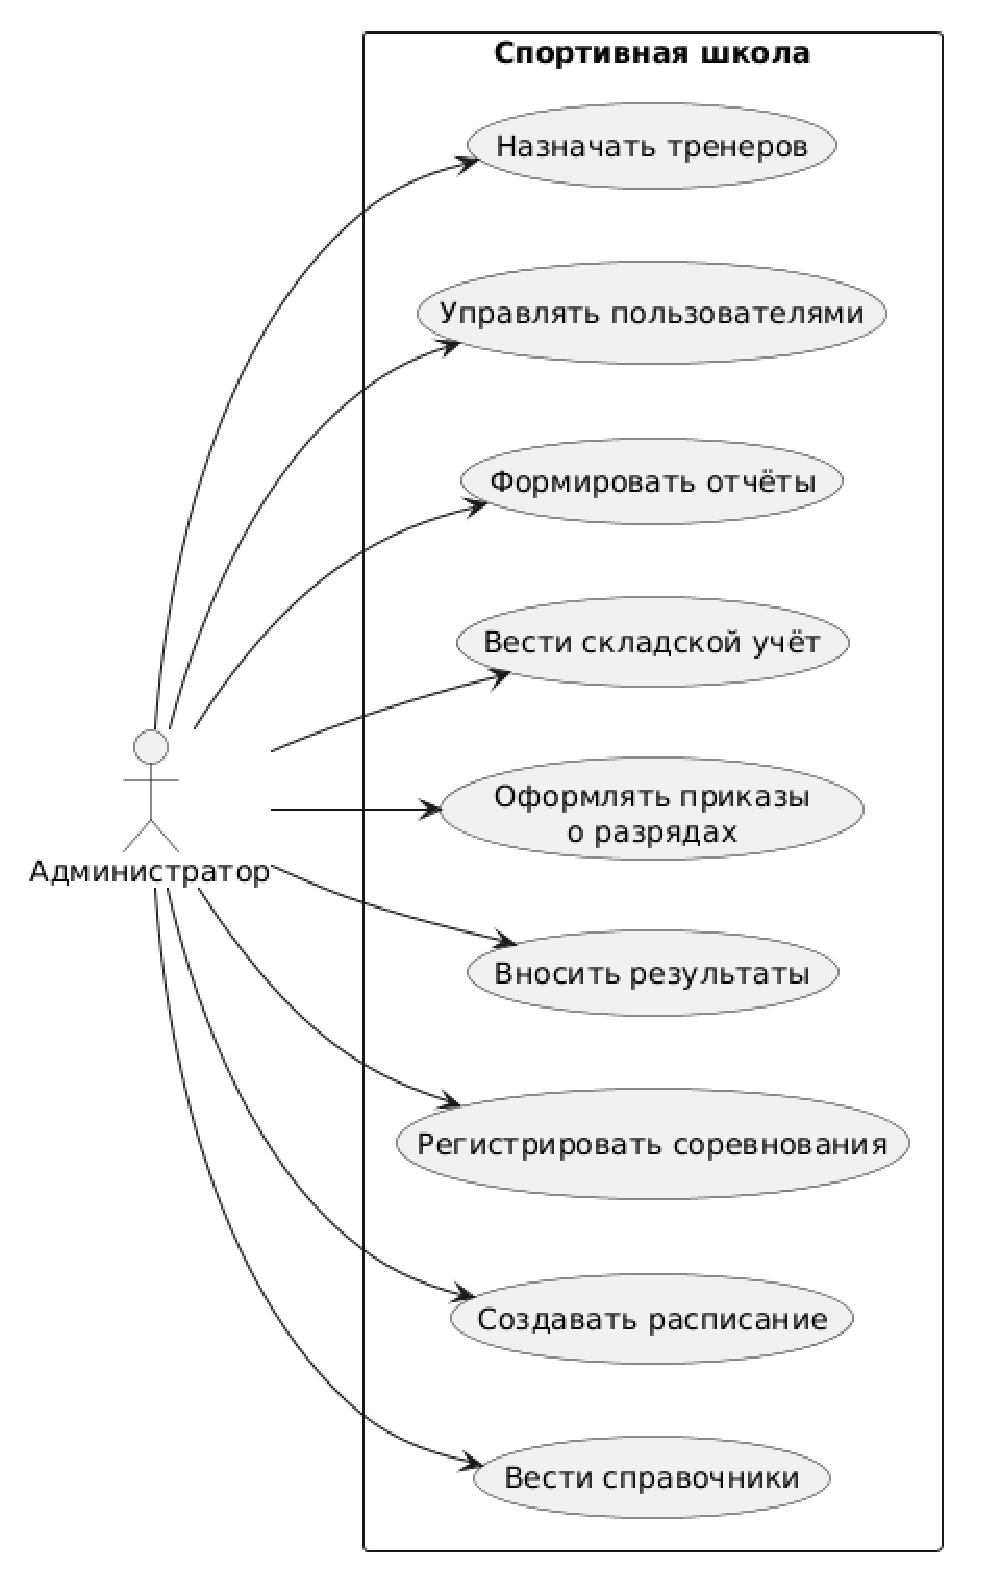
\includegraphics[width=0.9\textwidth]{images/diagramma_admin2.eps}
\end{center}
\begin{center}
	Рисунок 2.1 - Диаграмма прецедентов для администратора
\end{center}

На рисунке 2.2 представлена диаграмма прецедентов для роли «Тренер».

\begin{center}
	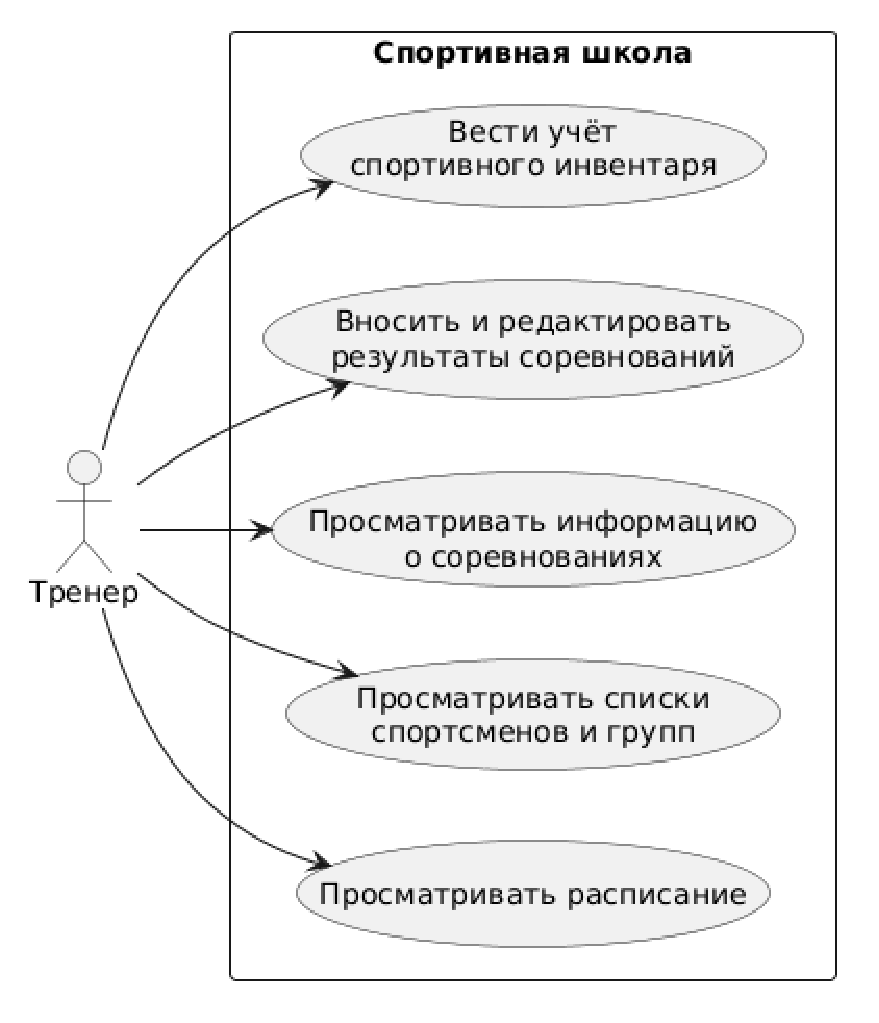
\includegraphics[width=0.9\textwidth]{images/diagramma_trener.eps}
\end{center}
\begin{center}
	Рисунок 2.2 - Диаграмма прецедентов для тренера
\end{center}

\vspace{0.3cm}

 Далее приведены детальные варианты использования для каждой роли, оформленные в виде текстовых сценариев.

\subsubsection{Вариант использования «Ведение справочника спортсменов»}

\textbf{Заинтересованные лица и их требования:} администратор желает поддерживать в актуальном состоянии список спортсменов школы.

\textbf{Предусловие:} открыт справочник «Спортсмены».

\textbf{Постусловие:} изменения сохранены в базе данных.

\textbf{Основной успешный сценарий:}

\begin{enumerate}
	\item Администратор открывает справочник «Спортсмены».
	\item Система отображает список всех спортсменов.
	\item Администратор нажимает «Создать» для добавления нового спортсмена.
	\item Система открывает форму элемента справочника.
	\item Администратор заполняет обязательные поля (фамилия, имя, отчество, дата рождения) и табличную часть с видами спорта и разрядами.
	\item Администратор нажимает «Записать и закрыть».
	\item Система сохраняет запись и обновляет список.
\end{enumerate}

\subsubsection{Вариант использования «Создание расписания занятий»}

\textbf{Заинтересованные лица и их требования:} администратор желает составить расписание тренировок на месяц.

\textbf{Предусловие:} открыт список документов «Расписание занятий».

\textbf{Постусловие:} документ проведен, записи в регистрах сформированы.

\textbf{Основной успешный сценарий:}

\begin{enumerate}
	\item Администратор создает новый документ «Расписание занятий».
	\item Система автоматически присваивает номер и устанавливает текущую дату.
	\item Администратор указывает месяц, на который составляется расписание.
	\item Администратор добавляет строки в табличную часть: выбирает тренера, группу, место проведения и указывает временные интервалы для каждого дня недели.
	\item Администратор нажимает «Провести и закрыть».
	\item Система проверяет заполнение обязательных полей.
	\item Документ проводится, формируются записи в регистрах сведений.
	\item Система закрывает форму документа.
\end{enumerate}

\textbf{Альтернативный сценарий (не заполнены обязательные поля):}

\begin{enumerate}
	\item Администратор не заполняет поле «Месяц» или не добавляет ни одной строки в табличную часть.
	\item Администратор нажимает «Провести и закрыть».
	\item Система выводит сообщение об ошибке: «Не заполнены обязательные реквизиты».
	\item Документ не проводится, форма остается открытой для исправления.
\end{enumerate}

\subsubsection{Вариант использования «Регистрация соревнования»}

\textbf{Заинтересованные лица и их требования:} администратор желает зарегистрировать новое соревнование.

\textbf{Предусловие:} открыт список документов «Соревнования».

\textbf{Постусловие:} соревнование зарегистрировано в системе.

\textbf{Основной успешный сценарий:}

\begin{enumerate}
	\item Администратор создает новый документ «Соревнования».
	\item Заполняет шапку: название, вид спорта, главный судья, статус, даты, место проведения.
	\item Заполняет табличную часть «Дисциплины»: добавляет дисциплины с указанием возрастной категории.
	\item Заполняет табличную часть «Участники»: добавляет спортсменов или команды с указанием дисциплины.
	\item Заполняет табличную часть «Судьи»: добавляет членов судейской коллегии с указанием роли.
	\item Администратор нажимает «Провести и закрыть».
	\item Система сохраняет и проводит документ.
\end{enumerate}

\textbf{Альтернативный сценарий (не заполнены обязательные поля):}

\begin{enumerate}
	\item Администратор не заполняет поле «Название» или «Вид спорта».
	\item Администратор нажимает «Провести и закрыть».
	\item Система выводит сообщение об ошибке с указанием незаполненных полей.
	\item Документ не проводится до устранения ошибок.
\end{enumerate}

\subsubsection{Вариант использования «Внесение результатов соревнований из файла»}

\textbf{Заинтересованные лица и их требования:} администратор желает ускорить ввод результатов, загрузив их из заранее подготовленного файла Excel.

\textbf{Предусловие:} открыт документ «Результаты соревнований».

\textbf{Постусловие:} табличная часть заполнена данными из файла.

\textbf{Основной успешный сценарий:}

\begin{enumerate}
	\item Администратор создает документ «Результаты соревнований» на основании документа «Соревнования».
	\item Администратор нажимает кнопку «Заполнить из файла».
	\item Система открывает диалог выбора файла.
	\item Администратор выбирает подготовленный файл формата Excel.
	\item Система считывает данные из файла, выполняет поиск участников и дисциплин по наименованию и заполняет табличную часть.
	\item Администратор проверяет корректность данных и проводит документ.
\end{enumerate}

\subsubsection{Вариант использования «Формирование отчета по расписанию»}

\textbf{Заинтересованные лица и их требования:} тренер желает просмотреть свое расписание на определенный период.

\textbf{Предусловие:} открыт раздел «Отчеты».

\textbf{Постусловие:} отчет сформирован и отображает актуальные данные.

\textbf{Основной успешный сценарий:}

\begin{enumerate}
	\item Тренер открывает отчет «Расписание занятий тренера».
	\item Система открывает форму с параметрами отчета.
	\item Тренер указывает период и выбирает себя из списка тренеров.
	\item Тренер нажимает «Сформировать».
	\item Система выполняет запрос к регистру сведений и выводит расписание в календарном виде.
\end{enumerate}

\subsubsection{Вариант использования «Назначение тренера на группу спортсменов»}

\textbf{Заинтересованные лица и их требования:} администратор желает закрепить тренера за группой спортсменов по определенному виду спорта.

\textbf{Предусловие:} открыт список документов «Приказ о назначении тренера».

\textbf{Постусловие:} документ проведен, запись в регистре сведений «Тренер спортсмена» сформирована.

\textbf{Основной успешный сценарий:}

\begin{enumerate}
	\item Администратор создает новый документ «Приказ о назначении тренера».
	\item Система автоматически присваивает номер и устанавливает текущую дату.
	\item Администратор выбирает вид спорта из справочника.
	\item Администратор выбирает тренера из справочника.
	\item Администратор указывает дату назначения.
	\item В табличной части администратор добавляет спортсменов из справочника.
	\item Администратор нажимает «Провести и закрыть».
	\item Система проверяет корректность заполнения и проводит документ, формируя записи в регистре сведений.
\end{enumerate}

\subsubsection{Вариант использования «Присвоение спортивного разряда»}

\textbf{Заинтересованные лица и их требования:} администратор желает оформить присвоение нового спортивного разряда группе спортсменов.

\textbf{Предусловие:} в системе имеются результаты соревнований, на основании которых может быть присвоен разряд.

\textbf{Постусловие:} приказ о присвоении разряда проведен, разряды спортсменов обновлены.

\textbf{Основной успешный сценарий:}

\begin{enumerate}
	\item Администратор открывает список документов «Заявка на присвоение разрядов» и создает новый документ.
	\item Администратор указывает вид спорта и желаемый разряд.
	\item В табличной части администратор добавляет спортсменов, указывая для каждого название соревнований, результат и ссылку на документ результатов.
	\item Администратор проводит заявку.
	\item На основании заявки администратор создает документ «Приказ о присвоении разряда».
	\item Администратор проверяет состав спортсменов и вид спорта в табличной части приказа.
	\item При необходимости администратор нажимает кнопку «Печать» для формирования официальной печатной формы приказа.
	\item Администратор нажимает «Провести и закрыть».
\end{enumerate}

\subsubsection{Вариант использования «Поступление спортивного инвентаря»}

\textbf{Заинтересованные лица и их требования:} администратор желает оприходовать поступивший от поставщика спортивный инвентарь.

\textbf{Предусловие:} открыт список документов «Поступление спортивного инвентаря».

\textbf{Постусловие:} документ проведен, остатки инвентаря в регистре накопления увеличены.

\textbf{Основной успешный сценарий:}

\begin{enumerate}
	\item Администратор создает новый документ «Поступление спортивного инвентаря».
	\item Система автоматически присваивает номер и устанавливает текущую дату.
	\item Администратор выбирает поставщика из справочника.
	\item В табличной части администратор добавляет строки: выбирает спортивный инвентарь из справочника и указывает количество.
	\item Администратор нажимает «Провести и закрыть».
	\item Система формирует приходные движения по регистру накопления «Спортивный инвентарь организации».
\end{enumerate}

\subsubsection{Вариант использования «Выдача спортивного инвентаря спортсмену»}

\textbf{Заинтересованные лица и их требования:} администратор желает зафиксировать выдачу инвентаря конкретному спортсмену или тренеру.

\textbf{Предусловие:} открыт список документов «Выдача спортивного инвентаря».

\textbf{Постусловие:} документ проведен, остатки инвентаря по материально-ответственному лицу увеличены, общие остатки уменьшены.

\textbf{Основной успешный сценарий:}

\begin{enumerate}
	\item Администратор создает новый документ «Выдача спортивного инвентаря».
	\item В табличной части администратор добавляет строки: выбирает инвентарь, указывает материально-ответственное лицо (спортсмена или тренера) и количество.
	\item Администратор нажимает «Провести и закрыть».
	\item Система формирует движения по регистру накопления: расход со склада и приход на материально-ответственное лицо.
\end{enumerate}

\textbf{Альтернативный сценарий (недостаточно инвентаря на складе):}

\begin{enumerate}
	\item Администратор пытается выдать количество инвентаря, превышающее текущий остаток.
	\item Система проверяет остатки по регистру накопления.
	\item Система выводит сообщение: «Недостаточно инвентаря на складе».
	\item Документ не проводится.
\end{enumerate}

\subsubsection{Вариант использования «Списание непригодного инвентаря»}

\textbf{Заинтересованные лица и их требования:} администратор желает списать инвентарь, пришедший в негодность.

\textbf{Предусловие:} открыт список документов «Списание спортивного инвентаря».

\textbf{Постусловие:} документ проведен, остатки инвентаря уменьшены.

\textbf{Основной успешный сценарий:}

\begin{enumerate}
	\item Администратор создает новый документ «Списание спортивного инвентаря».
	\item Администратор заполняет поле «Основание» (причина списания).
	\item В табличной части администратор добавляет строки: выбирает инвентарь и указывает количество.
	\item Администратор нажимает «Провести и закрыть».
	\item Система формирует расходные движения по регистру накопления.
\end{enumerate}

\subsubsection{Вариант использования «Просмотр общего расписания»}

\textbf{Заинтересованные лица и их требования:} администратор или тренер желает увидеть сводное расписание всех занятий за период.

\textbf{Предусловие:} открыт раздел «Отчеты».

\textbf{Постусловие:} отчет сформирован, расписание отображается в календарном виде с группировкой по видам спорта и тренерам.

\textbf{Основной успешный сценарий:}

\begin{enumerate}
	\item Пользователь открывает отчет «Расписание занятий общее».
	\item Система открывает форму с параметрами: период, тренер (необязательно).
	\item Пользователь указывает период (начало и конец месяца).
	\item При необходимости выбирает конкретного тренера для фильтрации.
	\item Пользователь нажимает «Сформировать».
	\item Система выполняет запрос к регистру сведений и выводит расписание в виде планировщика с иерархией: вид спорта, тренер, группа.
\end{enumerate}

\subsubsection{Вариант использования «Прикрепление файлов к документу»}

\textbf{Заинтересованные лица и их требования:} администратор желает прикрепить скан документа или иной файл к приказу или соревнованию.

\textbf{Предусловие:} открыт документ (приказ, соревнование), к которому требуется прикрепить файл.

\textbf{Постусловие:} файл сохранен в системе и связан с документом.

\textbf{Основной успешный сценарий:}

\begin{enumerate}
	\item Администратор открывает документ и нажимает кнопку «Вложенные файлы» на командной панели.
	\item Система открывает форму для работы с прикрепленными файлами.
	\item Администратор нажимает «Добавить» и выбирает файл на диске.
	\item Система загружает файл в информационную базу и связывает его с текущим документом.
	\item Администратор закрывает форму вложенных файлов.
\end{enumerate}

\subsubsection{Вариант использования «Отправка уведомления участникам соревнований»}

\textbf{Заинтересованные лица и их требования:} администратор желает оповестить участников соревнований по электронной почте.

\textbf{Предусловие:} открыт документ «Соревнования», в табличной части «Участники» указаны спортсмены с заполненными адресами электронной почты. В системе настроена учетная запись электронной почты.

\textbf{Постусловие:} письма отправлены всем участникам, имеющим e-mail.

\textbf{Основной успешный сценарий:}

\begin{enumerate}
	\item Администратор открывает документ «Соревнования».
	\item Нажимает кнопку «Отправить напоминание по эл. почте» на командной панели.
	\item Система собирает адреса электронной почты всех участников из табличной части.
	\item Система формирует текст письма, содержащий название соревнования, вид спорта, место и дату проведения.
	\item Система подключается к почтовому серверу и выполняет рассылку.
	\item Система выводит сообщение о результате отправки.
\end{enumerate}

\textbf{Альтернативный сценарий (отсутствуют адреса электронной почты):}

\begin{enumerate}
	\item Администратор нажимает кнопку «Отправить напоминание по эл. почте».
	\item Система проверяет наличие заполненных адресов у участников.
	\item Если ни у одного участника не указан e-mail, система выводит сообщение: «Нет получателей для отправки».
	\item Письма не отправляются.
\end{enumerate}

\textbf{Альтернативный сценарий (ошибка подключения к почтовому серверу):}

\begin{enumerate}
	\item Система пытается подключиться к почтовому серверу.
	\item Сервер недоступен или учетные данные неверны.
	\item Система выводит сообщение: «Ошибка при отправке. Не удалось подключиться к серверу».
	\item Письма не отправляются, документ остается в прежнем состоянии.
\end{enumerate}


\subsection{Требования к надежности}

Система должна обеспечивать надежную обработку и хранение данных как при обычной эксплуатации, так и при возникновении ошибок.

\textbf{Целостность данных.} Все операции проведения документов должны выполняться в рамках платформы 1С:Предприятие, что исключает сохранение частично заполненных данных при возникновении ошибок.

\textbf{Устойчивость к ошибкам.} Система должна корректно обрабатывать исключительные ситуации и выводить информативные сообщения пользователю без аварийного завершения работы.

\textbf{Валидация входных данных.} При заполнении форм документов и справочников должна выполняться проверка обязательных полей для предотвращения попадания некорректных записей в базу данных.

\textbf{Резервное копирование.} Для обеспечения сохранности данных должно выполняться регулярное резервное копирование информационной базы штатными средствами платформы 1С:Предприятие (выгрузка в формат .dt).

\subsection{Требования к информационной безопасности}

Система должна обеспечивать защиту данных и административного контура от несанкционированного доступа.

\textbf{Разграничение доступа.} Доступ к функциям системы должен определяться назначенной ролью пользователя (администратор или тренер). Административные функции (управление пользователями, настройка учетных записей почты) должны быть недоступны для роли «Тренер».

\textbf{Контроль уникальности.} Система должна обеспечивать автоматический контроль уникальности номеров документов и кодов справочников для предотвращения дублирования записей.

\textbf{Сохранность данных.} При аварийном завершении работы платформы внесенные данные не должны теряться благодаря механизму автоматического сохранения.

\subsection{Требования к программной и технической совместимости}

Система должна корректно функционировать в типовой среде развертывания учебной версии 1С:Предприятие.

\textbf{Операционная система.} Система должна работать под управлением операционных систем Windows 10 или Windows 11.

\textbf{Программные зависимости.} Для функционирования системы необходима установленная платформа «1С:Предприятие 8.3» (учебная версия). Для функции почтовых оповещений требуется доступ к сети Интернет.

\textbf{Требования к аппаратному обеспечению.} Система должна функционировать на компьютерах с характеристиками, соответствующими минимальным требованиям платформы 1С:Предприятие (процессор с тактовой частотой от 2 ГГц, оперативная память от 4 ГБ, свободное дисковое пространство от 10 ГБ).

\subsection{Требования к оформлению документации}

Разработка программной документации и программного изделия должна производиться согласно ГОСТ 19.102-77 и ГОСТ 34.601-90. Единая система программной документации.
	\section{Технический проект}

\subsection{Архитектура и взаимодействие компонентов программной системы}

Разработанная информационная система представляет собой конфигурацию для платформы «1С:Предприятие 8.3», функционирующую в режиме файловой информационной базы. Архитектура решения соответствует классической модели, заложенной в платформу: данные хранятся в объектах конфигурации (справочниках, документах, регистрах), бизнес-логика сосредоточена в программных модулях, а пользовательский интерфейс реализован в виде управляемого приложения.

Центральным принципом работы системы является событийная модель. Все значимые операции (составление расписания, проведение соревнований, движение инвентаря) оформляются в виде документов. В момент проведения документа платформа автоматически формирует записи в регистрах, обеспечивая тем самым целостность, непротиворечивость и хронологическую упорядоченность данных. Такой подход позволяет в любой момент времени получить актуальный срез информации, будь то расписание на конкретную дату или текущий остаток спортивного инвентаря.

Архитектура системы построена по трехуровневому принципу, соответствующему стандартам платформы 1С:Предприятие 8.3. Верхний уровень представления обеспечивает взаимодействие пользователей с системой через управляемый интерфейс. Средний уровень бизнес-логики содержит программные модули, реализующие обработку данных. Нижний уровень данных включает справочники, документы и регистры, хранящиеся в файловой базе данных. Файловый режим работы выбран в связи с небольшим количеством одновременно работающих пользователей, что позволило избежать необходимости развертывания выделенного сервера СУБД. Общая схема взаимодействия компонентов системы в рамках данной архитектуры представлена на рисунке 3.1.

\begin{center}
	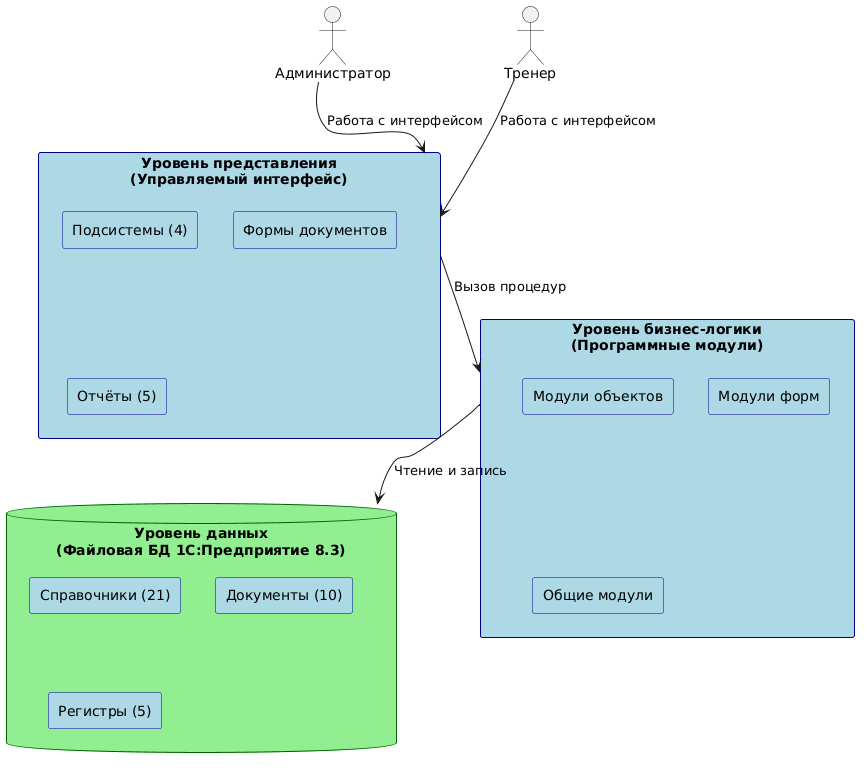
\includegraphics[width=0.9\textwidth]{images/ris3_1.png}
\end{center}
\begin{center}
{Рисунок 3.1 - Общая схема взаимодействия компонентов системы}
\end{center}

\subsection{Обоснование выбора платформы проектирования}

Платформа «1С:Предприятие 8.3» была выбрана в качестве среды разработки из-за совокупности факторов, позволяющие успешно выполнить проект.

Платформа предоставляет интегрированную среду быстрой разработки, включающую визуальные конструкторы форм, справочников и документов. Это позволило в сжатые сроки создать полнофункциональное приложение, не прибегая к программированию рутинных операций по созданию пользовательского интерфейса. Там, где требовалась нестандартная логика, использовался встроенный язык программирования, не уступающий современным процедурным языкам.

Наличие встроенной системы компоновки данных (СКД) дало возможность создавать аналитические отчеты различной сложности декларативно, без написания программного кода. Гибкая ролевая модель позволила реализовать разграничение прав доступа, критически важное для информационных систем с несколькими категориями пользователей. Наконец, возможность работы в файловом режиме избавила от необходимости развертывания и администрирования выделенного сервера СУБД, что особенно актуально для небольших организаций, таких как спортивные школы.

В качестве альтернатив рассматривались разработка с использованием веб-стека (языки Python, PHP, JavaScript) и различных СУБД, а также адаптация существующих коробочных решений. Однако эти варианты были отклонены по причинам значительно более высокой трудоемкости и стоимости разработки, а также ограниченной гибкости готовых продуктов.

\subsection{Структура конфигурации}

Информационная база системы включает в себя 21 справочник, 10 документов, 4 перечисления, 1 регистр накопления и 4 регистра сведений. Такая структура является типовой для прикладных решений на платформе 1С и обеспечивает четкое разделение данных на нормативно-справочную информацию (справочники), оперативные данные (документы) и агрегированные показатели (регистры).

Справочники образуют фундамент системы, храня информацию о спортсменах, тренерах, группах, видах спорта, помещениях и других сущностях. Документы, в свою очередь, фиксируют все изменения и события, происходящие в процессе работы школы. При проведении каждого документа формируются движения по регистрам, которые аккумулируют данные в разрезах, необходимых для последующего анализа и построения отчетов. Наглядное представление состава объектов конфигурации приведено на рисунке 3.2.

\begin{center}
	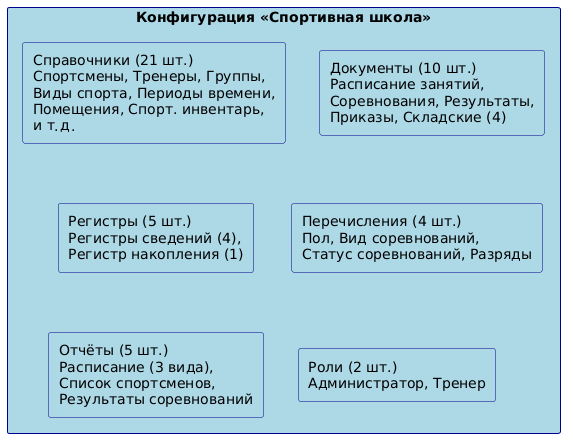
\includegraphics[width=0.9\textwidth]{images/ris3_2.png}
\end{center}
\begin{center}
{Рисунок 3.2 - Состав объектов конфигурации}
\end{center}

\subsection{Структура справочников}

Центральное место в системе занимает справочник «Спортсмены», аккумулирующий все сведения об учащихся. Помимо стандартных анкетных данных (ФИО, дата рождения, пол, контактная информация), он содержит табличную часть «Виды спорта», где для каждого спортсмена фиксируется вид спорта и присвоенный спортивный разряд. Это решение позволяет отразить ситуацию, когда один учащийся тренируется по нескольким видам и имеет по ним различные разряды.

Справочник «Тренеры» помимо анкетных данных содержит указание на специализацию (вид спорта) и должность. Это используется при составлении расписания для автоматической фильтрации тренеров по их профилю. Справочник «Группы» связывает учебные группы с конкретным видом спорта. Справочник «Периоды времени» задает временные слоты, из которых впоследствии формируется сетка расписания.

Ключевым классификатором является справочник «Виды спорта», выступающий владельцем для подчиненного ему справочника «Спортивные дисциплины». Такая связь позволяет для каждого вида спорта вести собственный уникальный перечень дисциплин.Это исключает смешение данных между разными видами спорта и упрощает фильтрацию при выборе дисциплины в документах «Соревнования» и «Результаты соревнований».

В таблице 3.1 приведен перечень основных справочников системы с указанием их назначения.

\vspace{0.5cm}
\noindent
{Таблица 3.1 - Основные справочники системы}

\vspace{0.2cm}
\noindent
\begin{tabular}{|p{5cm}|p{10.5cm}|}
	\hline
	{Справочник} & {Назначение} \\
	\hline
	Спортсмены & Хранение анкетных данных учащихся, видов спорта и разрядов \\
	\hline
	Тренеры & Хранение данных о тренерском составе, специализации \\
	\hline
	Группы & Перечень учебных групп с привязкой к виду спорта \\
	\hline
	Виды спорта & Классификатор видов спорта, владелец для дисциплин \\
	\hline
	Спортивные дисциплины & Перечень дисциплин, подчинен видам спорта \\
	\hline
	Периоды времени & Временные слоты для составления расписания \\
	\hline
	Помещения & Места проведения тренировок и соревнований \\
	\hline
	Спортивный инвентарь & Номенклатура инвентаря для складского учета \\
	\hline
	Спортивные разряды & Классификатор спортивных разрядов и званий \\
	\hline
	Поставщики & Организации, поставляющие спортивный инвентарь \\
	\hline
	Спортивные судьи & Данные о судейском составе \\
	\hline
	Статус соревнований & Классификатор уровней соревнований \\
	\hline
\end{tabular}

\newpage

Взаимосвязи между ключевыми сущностями системы представлены на рисунке 3.3.

\begin{center}
	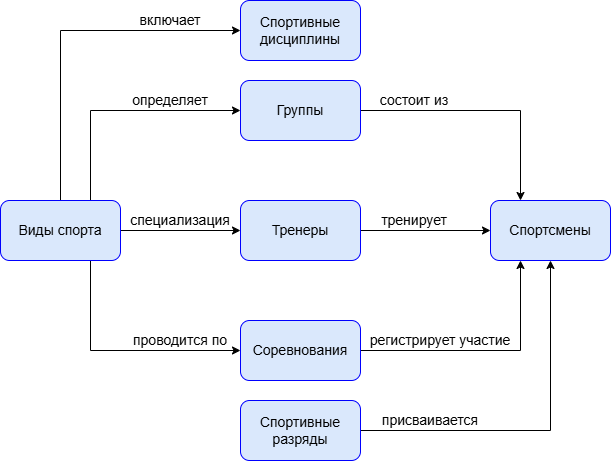
\includegraphics[width=0.9\textwidth]{images/er_diagramma2.png}
\end{center}
\begin{center}
{Рисунок 3.3 - Схема связи ключевых сущностей системы}
\end{center}

\subsection{Структура документов}

Основным операционным документом системы является «Расписание занятий», предназначенный для планирования тренировочного процесса на календарный месяц. Его табличная часть построена по принципу матрицы: строки определяют связку «тренер - группа - место проведения», а колонки соответствуют дням недели, в ячейках которых проставляются временные интервалы из справочника «Периоды времени». При проведении документ генерирует записи в регистрах сведений, делая расписание доступным для анализа в отчетах.

Документ «Соревнования» отличается сложной структурой, включающей три табличные части: «Дисциплины», «Участники» и «Судьи», что позволяет всесторонне описать спортивное мероприятие. На его основании вводится документ «Результаты соревнований», для которого реализована функция массовой загрузки данных из файлов Microsoft Excel, что значительно ускоряет работу при обработке большого количества результатов.

Цепочка оформления спортивных разрядов автоматизирована документами «Заявка на присвоение разрядов» и «Приказ о присвоении разряда». Последний имеет печатную форму, генерируемую по утвержденному шаблону.

Учет спортивного инвентаря реализован набором из четырех документов: «Поступление», «Выдача», «Возврат» и «Списание». Все они при проведении формируют движения по регистру накопления «Спортивный инвентарь организации».

В таблице 3.2 приведен полный перечень документов системы с указанием формируемых ими движений по регистрам.

\newpage

\noindent
{Таблица 3.2 - Документы системы и формируемые движения}
\par\vspace{0.2cm}
\noindent
\begin{tabular}{|p{6cm}|p{9.5cm}|}
		\hline
		{Документ} & {Формируемые движения (регистры)} \\
		\hline
		Расписание занятий & Регистры сведений «Расписание занятий», «Расписание занятий группы» \\
		\hline
		Приказ о назначении тренера & Регистр сведений «Тренер спортсмена» \\
		\hline
		Соревнования & Без движений (регистрация факта) \\
		\hline
		Результаты соревнований & Регистр сведений «Результаты соревнований» \\
		\hline
		Заявка на присвоение разрядов & Без движений (основание для приказа) \\
		\hline
		Приказ о присвоении разряда & Без движений (итоговый документ) \\
		\hline
		Поступление инвентаря & Регистр накопления «Спортивный инвентарь организации» (приход) \\
		\hline
		Выдача инвентаря & Регистр накопления «Спортивный инвентарь организации» (расход, приход на МОЛ) \\
		\hline
		Возврат инвентаря & Регистр накопления «Спортивный инвентарь организации» (приход, расход с МОЛ) \\
		\hline
		Списание инвентаря & Регистр накопления «Спортивный инвентарь организации» (расход) \\
		\hline
\end{tabular}
\vspace{0.4cm}

\subsection{Регистры}

Для накопления и хранения оперативных данных используются регистры двух типов.

Регистр накопления «Спортивный инвентарь организации» работает в режиме «Остатки» и позволяет в любой момент времени получить информацию о количестве каждой единицы инвентаря в разрезе материально-ответственных лиц (спортсменов или тренеров). Движения по регистру формируются автоматически при проведении складских документов.

Регистры сведений «Расписание занятий» и «Расписание занятий группы» являются хранилищем данных о расписании, заполняемым документом «Расписание занятий». На их основе строятся все отчеты по расписанию. Регистр «Тренер спортсмена» фиксирует историю назначений наставников, а регистр «Результаты соревнований» накапливает статистику выступлений. Использование периодических регистров сведений гарантирует сохранность всей истории изменений.

\subsection{Программная реализация}

Наиболее сложным в алгоритмическом плане является модуль формы документа «Расписание занятий». Для удобства заполнения расписания в документе используется табличная часть, где строки содержат тренера, группу и место проведения, а колонки соответствуют дням недели. В каждой ячейке пользователь выбирает временной интервал из справочника «Периоды времени». Проведение документа формирует записи в регистрах сведений, на основе которых в дальнейшем строятся отчеты.

Алгоритм программного заполнения планировщика относится к отчету «Расписание занятий общее», где данные уже не редактируются, а только отображаются. Для этого отчета используется элемент управления «Планировщик», заполнение которого выполняется полностью программно. Алгоритм построен на многоуровневом обходе иерархического результата запроса к регистру сведений. На первом уровне данные группируются по видам спорта, на втором - по тренерам, на третьем - по группам. Для каждого занятия вычисляются координаты на временной сетке планировщика, после чего создается визуальный элемент. Для улучшения восприятия различные уровни иерархии и сами занятия выделяются цветом. Внешний вид сформированного отчета представлен на рисунке 3.4.

Кроме того, программно реализована функция импорта данных в документ «Результаты соревнований» из файлов Excel. Процедура считывает табличный документ, выполняет сопоставление строк со справочниками спортсменов и дисциплин по наименованию и автоматически заполняет табличную часть документа.

\vspace{0.5cm}
\begin{center}
	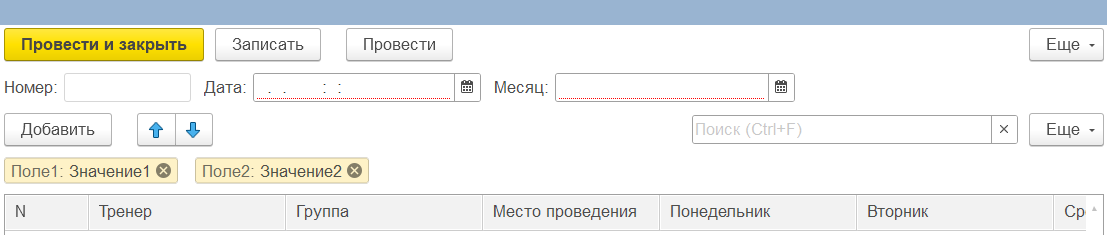
\includegraphics[width=1\textwidth, height=4.cm]{images/raspis_tabl.png}
\end{center}
\begin{center}
	{Рисунок 3.4 - Форма документа «Расписание занятий»}
\end{center}
\vspace{0.5cm}

\subsection{Пользовательский интерфейс}

Интерфейс системы реализован в полном соответствии с требованиями технического задания. Все четыре подсистемы, перечисленные в разделе 2.4, реализованы и функционируют. Каждая подсистема объединяет функционально связанные объекты, что делает навигацию интуитивно понятной и снижает время на поиск нужной команды.

Все формы документов и справочников выполнены в едином стиле управляемого приложения. Командные панели форм предоставляют пользователю как стандартные действия («Провести и закрыть», «Записать», «Провести»), так и дополнительные команды, специфичные для конкретных документов. Документ «Результаты соревнований» содержит кнопку «Заполнить из файла» для импорта данных из Excel, документ «Соревнования» - кнопку «Отправить напоминание по эл. почте», а документ «Приказ о присвоении разряда» - кнопку «Печать» для формирования официальной печатной формы.

Для визуализации расписания занятий применен специализированный элемент управления «Планировщик». По вертикальной оси планировщика располагается иерархический список с группировкой занятий по видам спорта, тренерам и группам. По горизонтальной оси отображается шкала дней месяца с детализацией по часам. Каждое занятие отображается в виде цветной плашки, что делает восприятие расписания наглядным и удобным для пользователя.

\subsection{Разграничение прав доступа}

Для обеспечения информационной безопасности и разграничения зон ответственности в системе реализованы две роли: «Администратор» и «Тренер». Разграничение прав выполнено штатными средствами платформы 1С:Предприятие через механизм ролей. Для каждой роли настроены индивидуальные права на чтение, просмотр, добавление, изменение и удаление по каждому объекту конфигурации.

Администратор обладает полным набором прав на все объекты конфигурации: может создавать, редактировать и удалять записи справочников, оформлять и проводить любые документы, формировать отчеты, управлять учетными записями пользователей и настраивать параметры электронной почты.

Тренер имеет доступ только к тем объектам, которые непосредственно связаны с его профессиональной деятельностью: просмотр расписания, справочников спортсменов и групп, просмотр информации о соревнованиях, внесение и редактирование результатов соревнований, учет спортивного инвентаря При этом для тренера полностью закрыт доступ к оформлению приказов и системным настройкам. При входе в систему платформа автоматически определяет роль пользователя и формирует интерфейс, отображая только те подсистемы и команды, которые разрешены данной роли.

\subsection{Обеспечение надежности и целостности данных}

Требования к надежности, сформулированные в техническом задании, реализованы в системе с использованием следующих механизмов.

Все операции, связанные с проведением документов, выполняются в рамках транзакций. В случае возникновения ошибки на любом этапе проведения документ все изменения автоматически откатываются, и документ остается в исходном состоянии.

Контроль уникальности номеров документов и кодов справочников реализован стандартными механизмами платформы. При попытке сохранить запись с уже существующим кодом или номером система автоматически блокирует операцию и выводит информативное сообщение.

Валидация входных данных выполняется на уровне платформы при проведении документов. Все обязательные реквизиты, отмеченные в конфигурации как подлежащие проверке, контролируются автоматически. При обнаружении незаполненных полей система выводит сообщение об ошибке и не позволяет провести документ до устранения недостатков.

Для обеспечения сохранности данных предусмотрено регулярное резервное копирование информационной базы штатными средствами платформы - выгрузка в формат .dt через конфигуратор. Данная операция позволяет сохранить как структуру конфигурации, так и все пользовательские данные в одном файле, который может быть загружен на другом компьютере для полного восстановления системы.

\subsection{Эксплуатация и развертывание}

Система функционирует в файловом режиме, что избавляет от необходимости развертывания и администрирования выделенного сервера СУБД. Для начала работы достаточно установить платформу «1С:Предприятие 8.3» (учебная версия) на компьютер под управлением операционной системы Windows 10 или Windows 11 и открыть файл информационной базы.

Для использования функции почтовых оповещений требуется наличие доступа к сети Интернет. Остальной функционал системы доступен полностью автономно, без подключения к внешним ресурсам.

Рекомендуемая минимальная конфигурация компьютера: процессор с тактовой частотой от 2 ГГц, оперативная память от 4 ГБ, свободное дисковое пространство от 10 ГБ. Данные характеристики соответствуют минимальным требованиям платформы «1С:Предприятие 8.3» и являются типовыми для большинства современных офисных компьютеров.

При необходимости масштабирования система может быть переведена в клиент-серверный режим с использованием СУБД PostgreSQL, что позволит увеличить количество одновременно работающих пользователей и повысить отказоустойчивость.
	\ifПрактика{}\else{
		\section{Рабочий проект}

В третьей главе были спроектированы архитектура, структура данных и пользовательский интерфейс системы. В данной главе приводится описание реализации разработанной конфигурации: описание процедур и функций, реализация ключевых алгоритмов, результаты функционального тестирования и инструкция по развертыванию.

\subsection{Спецификация программной реализации}

Программная часть системы включает процедуры и функции справочников, документов, форм, общие процедуры и отчеты.

\subsubsection{Процедуры справочников}

Для работы со справочниками системы реализованы процедуры обработки событий записи и проведения. Описание ключевых процедур приведено в таблице 4.1.

\vspace{0.5cm}

\newpage
\noindent
Таблица 4.1 - Процедуры проведения справочников

\vspace{0.2cm}
\noindent
\begin{tabular}{|p{5.75cm}|p{4.5cm}|p{5cm}|}
	\hline
	Процедура & Входные данные & Описание \\
	\hline
	ПередЗаписью (Спортсмены) & Объект справочника & Проверка заполнения обязательных полей (ФИО, дата рождения) \\
	\hline
	ПриЗаписи (Спортсмены) & Объект справочника & Автоматическое формирование наименования по ФИО \\
	\hline
	ПередЗаписью (Тренеры) & Объект справочника & Проверка заполнения специализации (Вид спорта) \\
	\hline
	ПриЗаписи (Тренеры) & Объект справочника & Автоматическое формирование наименования по ФИО \\
	\hline
	ПередЗаписью (Группы) & Объект справочника & Проверка заполнения вида спорта \\
	\hline
	ПриЗаписи (ПериодыВремени) & Объект справочника & Автоматическое формирование наименования по времени начала и окончания \\
	\hline
\end{tabular}

\vspace{0.4cm}

\subsubsection{Процедуры документов}

Для каждого документа реализована процедура обработки проведения, формирующая движения по регистрам. Описание ключевых процедур приведено в таблице 4.2.


\vspace{0.2cm}

\newpage
\noindent
Таблица 4.2 - Процедуры проведения документов

\vspace{0.2cm}
\noindent
\begin{tabular}{|p{5.7cm}|p{5.25cm}|p{4.3cm}|}
	\hline
	Процедура & Формируемые движения & Описание \\
	\hline
	ОбработкаПроведения (РасписаниеЗанятий) & Регистры сведений «Расписание занятий», «Расписание занятий группы» & Обход строк ТЧ, формирование записей для каждого дня недели \\
	\hline
	ОбработкаПроведения (ПриказОНазначении Тренера) & Регистр сведений «Тренер спортсмена» & Запись связки «тренер - спортсмен - вид спорта - дата» \\
	\hline
	ОбработкаПроведения (РезультатыСоревнований) & Регистр сведений «Результаты соревнований» & Обход строк ТЧ, запись результатов \\
	\hline
	ОбработкаПроведения (ПоступлениеИнвентаря) & Регистр накопления «Спортивный инвентарь организации» (приход) & Формирование приходных движений по каждой строке \\
	\hline
	ОбработкаПроведения (ВыдачаИнвентаря) & Регистр накопления «Спортивный инвентарь организации» (расход, приход на МОЛ) & Формирование расходных движений со склада и приходных - на МОЛ \\
	\hline
\end{tabular}
\vspace{0.4cm}

\subsubsection{Процедуры форм}

Формы системы содержат процедуры обработки событий элементов управления. Описание ключевых процедур приведено в таблице 4.3.

\newpage
\noindent
Таблица 4.3 - Процедуры форм

\vspace{0.2cm}
\noindent
\begin{tabular}{|p{5.25cm}|p{3.5cm}|p{6.5cm}|}
	\hline
	Процедура & Форма & Описание \\
	\hline
	ПриСозданииНаСервере & Расписание занятий & Установка текущей даты, инициализация реквизита «Месяц» \\
	\hline
	ПериодПриИзменении & Расписание занятий (общее) & Обновление планировщика при смене периода \\
	\hline
	ТренерПриИзменении & Расписание занятий (общее) & Фильтрация отображения по выбранному тренеру \\
	\hline
	ЗаполнитьИзФайла НаСервере & Результаты соревнований & Чтение Excel, поиск участников и дисциплин, заполнение ТЧ \\
	\hline
	ОтправитьНапоминание НаСервере & Соревнования & Сбор адресов, формирование письма, отправка через SMTP \\
	\hline
	УчастникиУчастник НачалоВыбора & Соревнования & Открытие формы выбора спортсменов с отбором по виду спорта \\
	\hline
\end{tabular}
\vspace{0.4cm}

\subsection{Реализация ключевых алгоритмов}

\subsubsection{Алгоритм заполнения планировщика расписания}

Алгоритм реализован в модуле формы отчета «Расписание занятий общее» и выполняет следующие шаги:

\begin{enumerate}
	\item Инициализация планировщика: очистка измерений и элементов, настройка цветовой схемы шкалы времени.
	\item Формирование и выполнение запроса к регистру сведений «Расписание занятий» с группировкой по полям «Вид спорта», «Тренер», «Группа».
	\item Обход результата запроса по первому уровню группировки (Вид спорта). Для каждого вида спорта создается элемент измерения верхнего уровня с зеленым цветом фона.
	\item Обход результата по второму уровню группировки (Тренер). Для каждого тренера создается вложенный элемент измерения с сиреневым цветом фона.
	\item Обход результата по третьему уровню группировки (Группа). Для каждой группы создается вложенный элемент измерения с желтым цветом фона.
	\item Для каждого занятия (конечная запись) вычисляются координаты на временной шкале: начало = Дата + Час × 3600 + Минута × 60, конец = Дата + Час × 3600 + Минута × 60. Создается элемент планировщика с золотистым цветом фона и текстом, содержащим период времени и место проведения.
	\item Привязка элемента планировщика к соответствующим измерениям через фиксированное соответствие.
\end{enumerate}

Полный программный код процедуры приведен в приложении А.

\subsubsection{Алгоритм загрузки результатов соревнований из Excel}

Алгоритм реализован в модуле формы документа «Результаты соревнований» и выполняет следующие шаги:

\begin{enumerate}
	\item Получение адреса файла во временном хранилище.
	\item Создание временного файла на диске и запись в него данных из хранилища.
	\item Чтение файла в объект «ТабличныйДокумент».
	\item Построение запроса на основе области данных табличного документа (начиная со второй строки, так как первая содержит заголовки).
	\item Обход результата запроса. Для каждой строки выполняется поиск участника и дисциплины по наименованию в соответствующих справочниках.
	\item Очистка табличной части документа и последовательное заполнение строк. Для каждой строки заполняются поля: Участник, Дисциплина, Результат, Место.
\end{enumerate}

Полный программный код процедуры приведен в приложении А.

\subsubsection{Алгоритм отправки почтовых уведомлений участникам соревнований}

Алгоритм реализован в модуле формы документа «Соревнования» и выполняет следующие шаги:

\begin{enumerate}
	\item Сбор адресов электронной почты всех участников из табличной части «Участники». Пропуск записей с незаполненным адресом.
	\item Проверка полученного массива: если нет ни одного получателя, то вывод сообщения об ошибке и завершение.
	\item Получение системной учетной записи электронной почты из справочника «Учетные записи электронной почты».
	\item Формирование параметров подключения к SMTP-серверу: адрес сервера, порт, логин, пароль.
	\item Формирование текста письма, содержащего название соревнования, вид спорта, место и дату проведения.
	\item Создание объекта «ИнтернетПочтовоеСообщение», заполнение темы, отправителя, получателей и текста письма.
	\item Подключение к почтовому серверу, отправка сообщения, отключение от сервера.
	\item Обработка исключений: при ошибке подключения или отправки  вывод сообщения с описанием ошибки.
\end{enumerate}

Полный программный код процедуры приведен в приложении А.

\subsubsection{Алгоритм формирования печатной формы приказа о присвоении разряда}

Алгоритм реализован в макете печатной формы документа «Приказ о присвоении разряда» и выполняет следующие шаги:

\begin{enumerate}
	\item Получение данных документа: номер, дата, разряд.
	\item Обход строк табличной части «Виды спорта». Для каждой строки получение вида спорта и спортсмена.
	\item Группировка спортсменов по видам спорта.
	\item Заполнение области печатной формы: наименование организации, заголовок приказа, табличная часть со списком спортсменов.
	\item Вывод печатной формы в режиме предварительного просмотра.
\end{enumerate}

\subsection{Функциональное тестирование}

Для проверки работоспособности разработанной системы было проведено функциональное тестирование. Проверялись основные сценарии использования: создание и проведение документов, корректность формирования движений по регистрам, работа отчетов, загрузка данных из Excel, разграничение прав доступа. На рисунках 4.1 - 4.7 представлены экранные формы системы, иллюстрирующие выполнение тестовых сценариев.

\subsubsection{Тестовый сценарий: создание и проведение расписания занятий}

\textbf{Предусловие:} система запущена, пользователь авторизован с ролью «Администратор».

\textbf{Тестовый случай:} пользователь создает новый документ «Расписание занятий», устанавливает месяц «Май 2026», добавляет пять строк с указанием тренера, группы, места проведения и временных интервалов по дням недели. Нажимает «Провести и закрыть».

\textbf{Ожидаемый результат:} документ проведен, в регистрах сведений «Расписание занятий» и «Расписание занятий группы» сформированы записи. Отчет «Расписание занятий общее» отображает введенные данные.

\textbf{Результат:} тест пройден успешно.

\vspace{1cm}
\begin{center}
	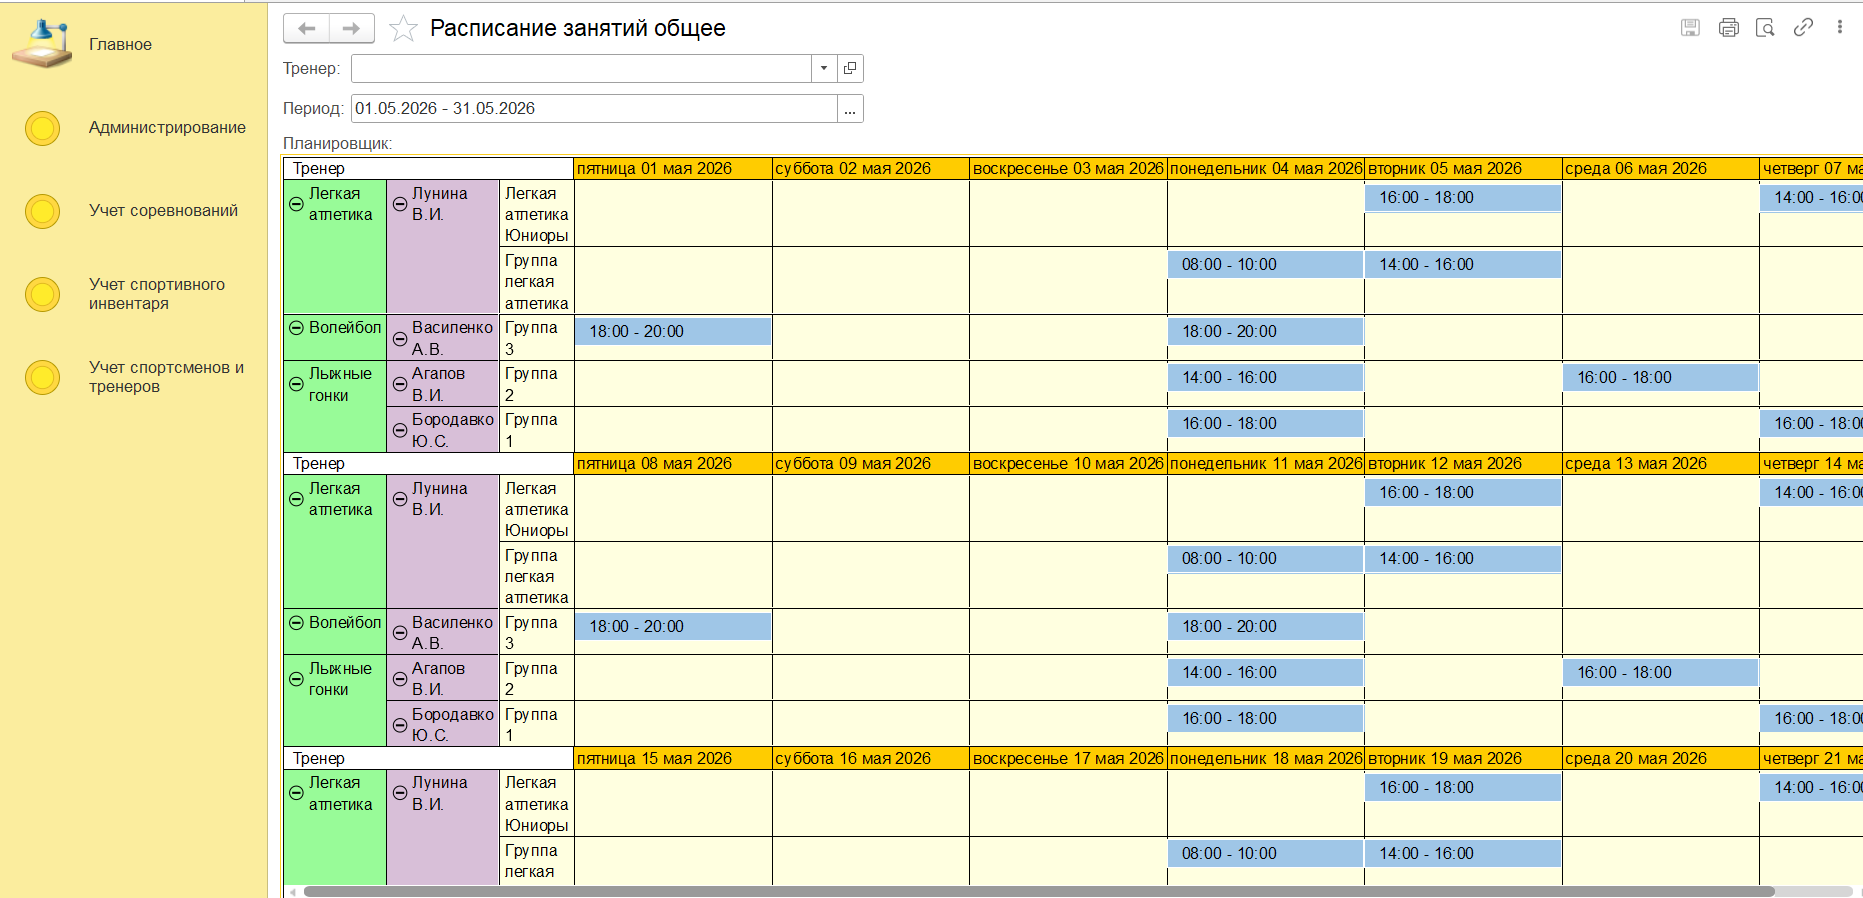
\includegraphics[width=0.9\textwidth]{images/raspis_zanatiy_rab_proeckt.png}
\end{center}
\begin{center}
	{Рисунок 4.1 - Отчет «Расписание занятий общее»}
\end{center}
\vspace{0.5cm}

\subsubsection{Тестовый сценарий: загрузка результатов соревнований из Excel}

\textbf{Предусловие:} система запущена, подготовлен файл Excel с результатами (12 строк с данными участников, дисциплин и результатов).

\textbf{Тестовый случай:} пользователь открывает документ «Результаты соревнований», нажимает «Заполнить из файла», выбирает подготовленный файл.

\textbf{Ожидаемый результат:} табличная часть документа заполнена данными из файла. Участники и дисциплины корректно сопоставлены со справочниками. Документ можно провести.

\textbf{Результат:} тест пройден успешно.

\vspace{1cm}
\begin{center}
	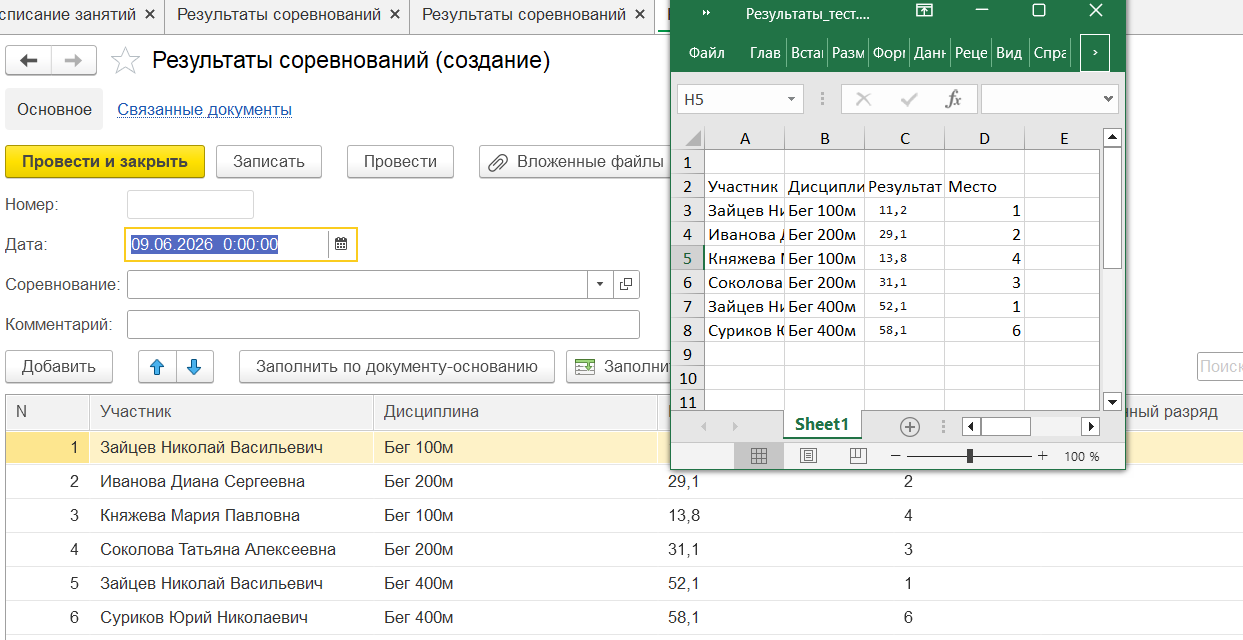
\includegraphics[width=0.9\textwidth]{images/rez_sorev1.png}
\end{center}
\begin{center}
	{Рисунок 4.2 - Форма документа «Результаты соревнований»}
\end{center}
\vspace{0.5cm}

\subsubsection{Тестовый сценарий: выдача инвентаря при недостатке на складе}

\textbf{Предусловие:} текущий остаток инвентаря «Палки Swix 155см» составляет 1 единицу.

\textbf{Тестовый случай:} пользователь создает документ «Выдача спортивного инвентаря», указывает инвентарь ««Палки Swix 155см», количество 5.

\textbf{Ожидаемый результат:} система выводит сообщение «Не удалось провести "Выдача спортивного инвентаря» В организации 1 из 5. Не хватает 4». Документ не проводится.

\textbf{Результат:} тест пройден успешно.

\vspace{1cm}
\begin{center}
	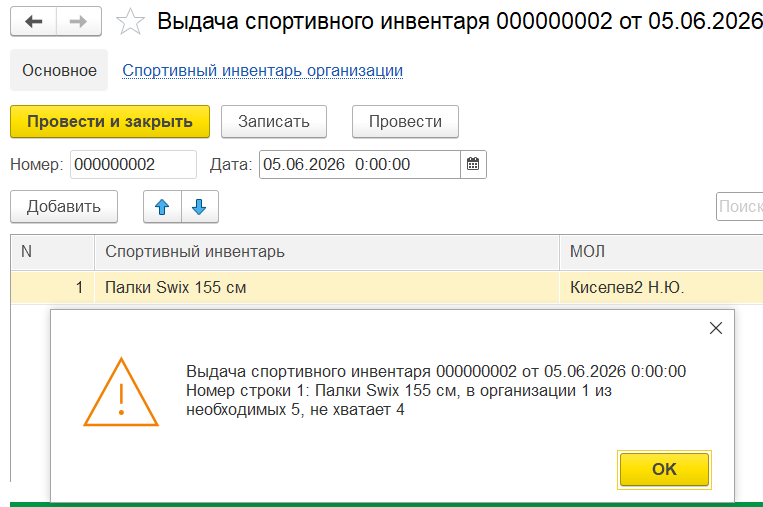
\includegraphics[width=0.9\textwidth]{images/vidacha.png}
\end{center}
\begin{center}
	{Рисунок 4.3 - «Выдача инвентаря»}
\end{center}
\vspace{0.5cm}

\subsubsection{Тестовый сценарий: формирование печатной формы приказа}

\textbf{Предусловие:} в системе имеется проведенный документ «Приказ о присвоении разряда» с заполненной табличной частью.

\textbf{Тестовый случай:} пользователь открывает документ и нажимает кнопку «Печать».

\textbf{Ожидаемый результат:} система формирует печатную форму приказа, содержащую наименование организации, номер и дату приказа, список спортсменов с видами спорта. Печатная форма открывается в режиме предварительного просмотра.

\textbf{Результат:} тест пройден успешно.

\vspace{1cm}
\begin{center}
	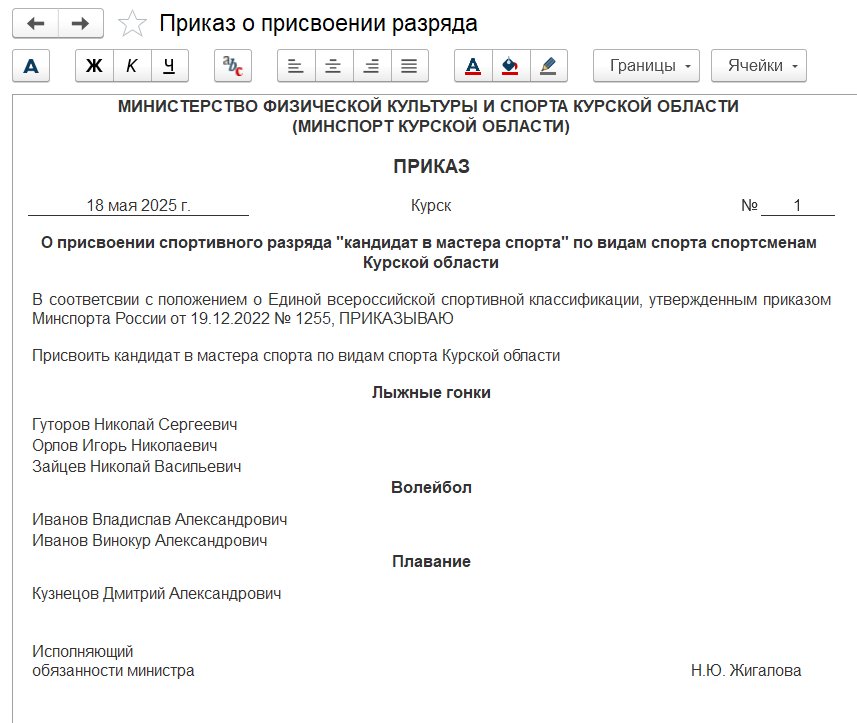
\includegraphics[width=0.9\textwidth]{images/prisvoenie_razr.png}
\end{center}
\begin{center}
	{Рисунок 4.4 - Печатная форма приказа о присвоении разряда}
\end{center}
\vspace{0.5cm}

\subsubsection{Тестовый сценарий: прикрепление файла к документу}

\textbf{Предусловие:} открыт документ «Соревнования», на диске имеется файл для прикрепления.

\textbf{Тестовый случай:} пользователь нажимает кнопку «Вложенные файлы», в открывшейся форме нажимает «Загрузить с диска» и выбирает файл с диска.

\textbf{Ожидаемый результат:} файл загружен в информационную базу и связан с документом. При повторном открытии формы вложенных файлов добавленный файл отображается в списке.

\textbf{Результат:} тест пройден успешно.

\vspace{1cm}
\begin{center}
	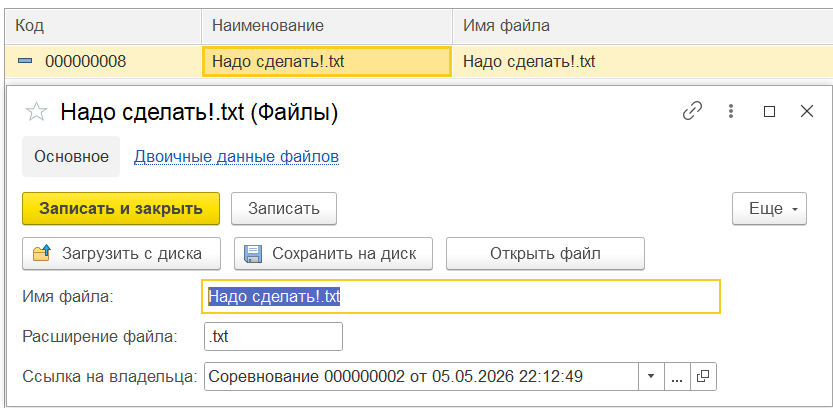
\includegraphics[width=0.9\textwidth]{images/fail.png}
\end{center}
\begin{center}
	{Рисунок 4.5 - Прикрепление файла}
\end{center}
\vspace{0.5cm}

\subsubsection{Тестовый сценарий: отправка почтового уведомления}

\textbf{Предусловие:} открыт документ «Соревнования» с участниками, у которых заполнены адреса электронной почты. В системе настроена учетная запись почты.

\textbf{Тестовый случай:} пользователь нажимает кнопку «Отправить напоминание по эл. почте».

\textbf{Ожидаемый результат:} система формирует письма и отправляет их участникам. Выводится сообщение о результате отправки.

\textbf{Результат:} тест пройден успешно (отправка выполнена, письма доставлены).

\vspace{1cm}
\begin{center}
	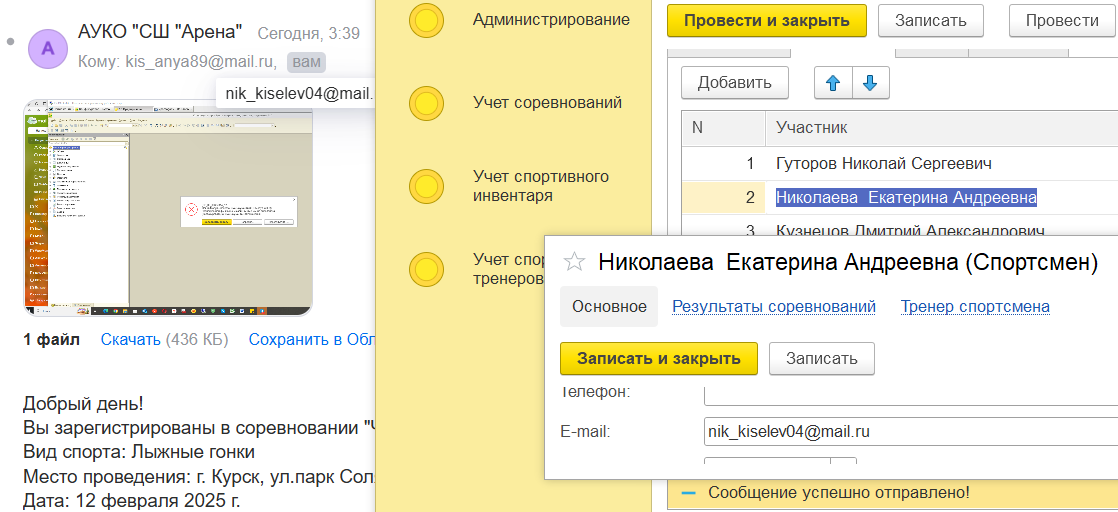
\includegraphics[width=0.9\textwidth]{images/uvedomlenie.png}
\end{center}
\begin{center}
	{Рисунок 4.6 - Отправка почтового уведомления}
\end{center}
\vspace{0.5cm}

\subsubsection{Тестовый сценарий: проверка разграничения прав доступа}

\textbf{Предусловие:} в системе создан пользователь с ролью «Тренер».

\textbf{Тестовый случай:} пользователь входит в систему под учетной записью тренера.

\textbf{Ожидаемый результат:} интерфейс отображает только подсистемы «Учет спортсменов и тренеров», «Учет соревнований» и «Учет спортивного инвентаря». Подсистема «Администрирование» не отображаются. 

\textbf{Результат:} тест пройден успешно.

\vspace{1cm}
\begin{center}
	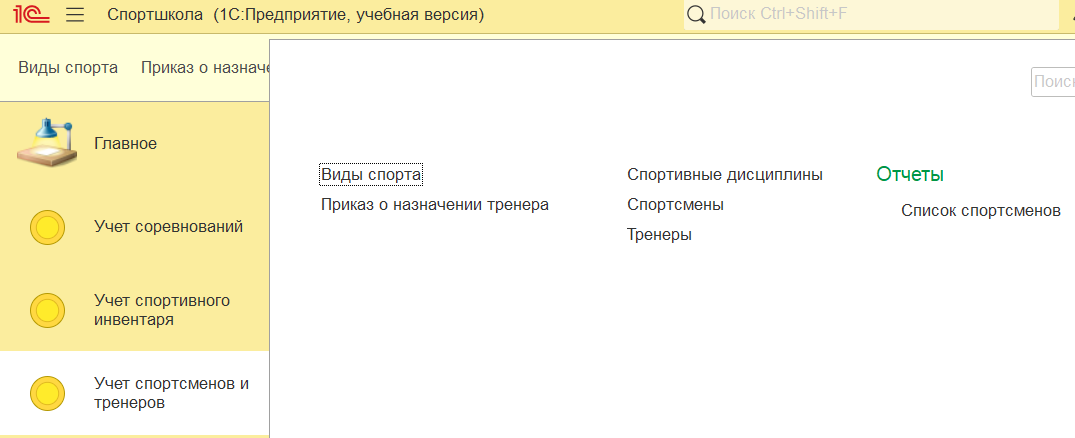
\includegraphics[width=0.9\textwidth]{images/vid_trener.png}
\end{center}
\begin{center}
	{Рисунок 4.7 - Интерфейс системы под ролью «Тренер»}
\end{center}
\vspace{0.5cm}

Рекомендуемая минимальная конфигурация компьютера: процессор с тактовой частотой от 2 ГГц, оперативная память от 4 ГБ, свободное дисковое пространство от 10 ГБ.
		\newpage
\begin{center}
	{ЗАКЛЮЧЕНИЕ}
\end{center}

В ходе выполнения выпускной квалификационной работы была разработана информационная система на платформе «1С:Предприятие 8.3» для комплексного учета деятельности спортивной организации. Разработанная конфигурация позволяет автоматизировать ключевые процессы спортивной организации и обеспечивает удобный доступ к информации для различных категорий пользователей.

На этапе анализа предметной области была охарактеризована деятельность спортивной организации на примере спортивной школы, выявлены основные бизнес-процессы, требующие автоматизации, и проведен обзор существующих программных решений. Результатом анализа стало обоснование необходимости разработки собственной конфигурации, полностью адаптированной под нужды спортивного учреждения.

В соответствии с техническим заданием в системе реализованы все заявленные функции:

\begin{enumerate}
	\item Управление данными о спортсменах и тренерах: справочники позволяют вести анкетные данные, фиксировать виды спорта и присвоенные разряды для спортсменов, а также специализацию и должность для тренеров.
	\item Составление и ведение расписания занятий: документ «Расписание занятий» обеспечивает планирование тренировок на месяц с детализацией по дням недели, тренерам, группам и местам проведения.
	\item Управление соревнованиями: документ «Соревнования» позволяет регистрировать спортивные мероприятия с указанием трех табличных частей: дисциплины, участники и судьи.
	\item Учет результатов соревнований: документ «Результаты соревнований», создаваемый на основании соревнований, обеспечивает ввод и хранение результатов с возможностью загрузки из файлов Excel.
	\item Оформление приказов на присвоение разрядов: «Приказ о присвоении разряда» автоматизирует процесс присвоения спортивных разрядов, имеет печатную форму.
	\item Складской учет спортивного инвентаря: четыре складских документа (поступление, выдача, возврат, списание) формируют движения по регистру накопления, позволяя получать актуальные остатки в любой момент.
	\item Формирование отчетности: реализованы отчеты «Расписание занятий общее», «Расписание занятий группы», «Расписание занятий тренера», «Список спортсменов» и «Результаты соревнований».
	\item Разграничение доступа: система поддерживает две роли: администратор (полный доступ) и тренер (ограниченный доступ без права работы со складскими документами, приказами и настройками).
	\item Отправка уведомлений: реализована рассылка уведомлений участникам соревнований по электронной почте.
\end{enumerate}

Созданная конфигурация включает 21 справочник, 10 документов, 4 перечисления, 1 регистр накопления и 4 регистра сведений. Интерфейс системы разделен на четыре подсистемы в соответствии с требованиями технического задания: «Учет спортсменов и тренеров», «Учет соревнований», «Учет спортивного инвентаря» и «Администрирование». Все формы выполнены в едином стиле управляемого приложения.

Практическая значимость работы заключается в создании готового к внедрению программного продукта, позволяющего сократить временные затраты на ведение документации, повысить качество планирования тренировочного процесса и обеспечить руководство спортивной организации актуальной информацией для принятия управленческих решений.

Дальнейшее развитие системы может быть направлено на расширение функционала: добавление модуля учета посещаемости, реализацию личного кабинета спортсмена с доступом через веб-интерфейс, интеграцию с мобильными приложениями, а также внедрение автоматизированного тестирования на базе фреймворка Vanessa Automation.

Таким образом, поставленные цели и задачи выпускной квалификационной работы выполнены в полном объеме. Разработанная информационная система готова к внедрению в деятельность спортивной организации.
	}\fi
	\addcontentsline{toc}{section}{СПИСОК ИСПОЛЬЗОВАННЫХ ИСТОЧНИКОВ}

\begin{thebibliography}{99}
	
	% === Книги по 1С:Предприятие ===
	
	\bibitem{radchenko} Радченко, М. Г. 1С:Предприятие 8.3. Практическое пособие разработчика. Примеры и типовые приемы / М. Г. Радченко, Е. Ю. Хрусталева. - 3-е изд. - Москва : 1С-Паблишинг, 2023. - 983 с. - ISBN 978-5-9677-3268-3. - Текст : непосредственный.
	
	\bibitem{hrustaleva_skd} Хрусталева, Е. Ю. Разработка сложных отч-тов в 1С:Предприятии 8. Система компоновки данных / Е. Ю. Хрусталева. - 4-е изд. - Москва : 1С-Паблишинг, 2024. - 485 с. - ISBN 978-5-9677-3448-9. - Текст : непосредственный.
	
	\bibitem{hrustaleva_query} Хрусталева, Е. Ю. Язык запросов 1С:Предприятия 8.3 / Е. Ю. Хрусталева. - Москва : 1С-Паблишинг, 2025. - 378 с. - ISBN 978-5-9677-3476-2. - Текст : непосредственный.
	
	\bibitem{chrustaleva_conf} Хрусталева, Е. Ю. Расширения конфигураций. Адаптация прикладных решений с сохранением поддержки в облаках и на земле. Разработка в системе «1С:Предприятие 8.3» / Е. Ю. Хрусталева. - 3-е изд., стереотипное. - Москва : 1С-Паблишинг, 2022. - 297 с. - ISBN 978-5-9677-3171-6. - Текст : непосредственный.
	
	\bibitem{filimonova} Филимонова, Е. В. Разработка и реализация конфигураций в системе 1С:Предприятие / Е. В. Филимонова. - Москва : Синергия, 2020. - 210 с. - ISBN 978-5-4257-0502-0. - Текст : непосредственный.
	
	\bibitem{marchenko} Марченко, И. О. Разработка системы управления предприятием на платформе «1С:Предприятие 8.3» / И. О. Марченко, М. Л. Перевертайло. - Новосибирск : Изд-во НГТУ, 2018. - 116 с. - ISBN 978-5-7782-3714-8. - Текст : непосредственный.
	
	\bibitem{kashaev} Кашаев, С. М. 1С:Предприятие 8.3. Программирование и визуальная разработка / С. М. Кашаев. - Санкт-Петербург : БХВ-Петербург, 2015. - 336 с. - ISBN 978-5-9775-2806-1. - Текст : непосредственный.
	
	\bibitem{gladkiy} Гладкий, А. 1С:Бухгалтерия для начинающих / А. Гладкий. - Санкт-Петербург : Питер, 2013. - 336 с. - ISBN 978-5-496-00087-1. - Текст : непосредственный.
	
	\bibitem{gabec} Габец, А. П. Реализация прикладных задач в системе "1С:Предприятие 8.2" / А. П. Габец, Д. В. Козырев, Д. С. Кухлевский, Е. Ю. Хрусталева. - Москва : 1С-Паблишинг, 2010. - 715 с. - ISBN 978-5-9677-1387-3. - Текст : непосредственный.
	
	\bibitem{gartvitsch} Гартвич, А. В. Бухгалтерский учет в 1С:Бухгалтерия 8.3. / А. В. Гартвич. - Санкт-Петербург : БХВ-Петербург, 2015. - 285 с. - ISBN 978-5-9775-3498-7. - Текст : непосредственный.
	
	\bibitem{skorohod} Скороход, С. В. Программирование на платформе 1С:Предприятие 8.3 / С. В. Скороход. - Ростов-на-Дону ; Таганрог : Издательство Южного федерального университета, 2019. - 137 с. - ISBN 978-5-9275-3315-2. - Текст : непосредственный.
	
	\bibitem{goncharov} Гончаров, Д. И. Решение специальных прикладных задач в 1С:Предприятии 8.2 / Д. И. Гончаров, Е. Ю. Хрусталева. - Москва : 1С-Паблишинг, 2012. - 300 с. - ISBN 978-5-9677-1611-9. - Текст : непосредственный.
	
	\bibitem{kaschaev} Кашаев, С. М. Программирование в 1С:Предприятие 8.3 / С. М. Кашаев. - Санкт-Петербург : Питер, 2014. - 304 с. - ISBN 978-5-496-01234-8. - Текст : непосредственный.
	
	\bibitem{nosova} Носова, Л. С. Информационные технологии в управлении образованием / Л. С. Носова. - Челябинск : Изд-во Южно-Уральского гос. гуманитарно-пед. ун-та, 2016. - 144 с. - ISBN 978-5-906908-21-6. - Текст : непосредственный.
	
	\bibitem{titenko} Титенко, Е. А. Автоматизированные информационные системы и интеллектуальные технологии / Е. А. Титенко, Н. В. Евтеева, Л. И. Гусева, С. С. Костюков. - Курск : Юго-Западный гос. ун-т, 2013. - 131 с. - ISBN 978-5-7681-0868-7. - Текст : непосредственный.
	
	\bibitem{kochura} Кочура, Е. П. Экономическая информатика / Е. П. Кочура, В. В. Серебровский. - Курск : Юго-Западный гос. ун-т, 2013. - 161 с. - ISBN 978-5-7681-0883-0. - Текст : непосредственный.
	
	\bibitem{granina} Грянина, Е. А. Секреты профессиональной работы с «1С:Зарплата и управление персоналом 8, редакция 3». Кадровый учет, экономика и охрана труда / Е. А. Грянина, С. Г. Змиевская. - Москва : 1С-Паблишинг, 2021. - 1002 с. - ISBN 978-5-9677-3090-0. - Текст : непосредственный.
	
	\bibitem{tschistov} Чистов, Д. В. Факты хозяйственной жизни в «1С:Бухгалтерии 8» / Д. В. Чистов, В. А. Матчинов. - Изд. 2. - Москва : 1С-Паблишинг, 2025. - 477 с. - ISBN 978-5-9677-3517-2. - Текст : непосредственный.
	
	\bibitem{radchenko_chrust} Радченко, М. Г. 1С:Предприятие 8.3. Практическое пособие разработчика. Используем 1С:EDT. Издание 2, стереотипное / М. Г. Радченко, Е. Ю. Хрусталева. - Москва : 1С-Паблишинг, 2026. - 1160 с. - ISBN 978-5-9677-3623-0. - Текст : непосредственный.
	
	\bibitem{ageronok} Ажеронок, В. А. Разработка интерфейса прикладных решений на платформе «1С:Предприятие 8». Издание 2, стереотипное / В. А. Ажеронок, А. В. Островерх, М. Г. Радченко, Е. Ю. Хрусталева. - Москва : 1С-Паблишинг, 2024. - 902 с. - ISBN 978-5-9677-3359-8. - Текст : непосредственный. 
	
	\bibitem{radchenko_nachalo} Радченко, М. Г. 1С:Программирование для начинающих. Детям и родителям, менеджерам и руководителям. Разработка в системе «1С:Предприятие 8.3» / М. Г. Радченко. - 2-е изд., стереотипное. - Москва : 1С-Паблишинг, 2022. - 781 с. - ISBN 978-5-9677-3172-3. - Текст : непосредственный.
	
	\bibitem{chrustaleva} Хрусталева, Е. Ю. Технологии интеграции «1С:Предприятия 8.3» / Е. Ю. Хрусталева. - 2-е изд., стереотипное. - Москва : 1С-Паблишинг, 2023. - 503 с. - ISBN 978-5-9677-3303-1. - Текст : непосредственный.
	
	\bibitem{chrustaleva_sistema} Хрусталева, Е. Ю. Система взаимодействия. Коммуникации в бизнес-приложениях. Разработка в системе «1С:Предприятие 8.3» / Е. Ю. Хрусталева. - Москва : 1С-Паблишинг, 2019. - 130 с. - ISBN 978-5-9677-2869-3. - Текст : непосредственный.
	
	
	
	% === Управление спортивными организациями ===
	
	\bibitem{filippov} Филиппов, С. С. Менеджмент физической культуры и спорта / С. С. Филиппов. - 6-е изд., перераб. и доп. - Москва : Юрайт, 2023. - 255 с. - ISBN 978-5-534-17685-8. - Текст : непосредственный.
	
	\bibitem{matveev} Матвеев, Л. П. Теория и методика физической культуры / Л. П. Матвеев. - 5-е изд., стереотипное. - Москва : Спорт, 2025. - 520 с. - ISBN 978-5-907601-90-1. - Текст : непосредственный.
	
	\bibitem{grigorieva} Григорьева, И. И. Образование и спортивная подготовка: процессы модернизации. Вопросы и ответы. Часть 1. Организация тренировочного процесса / И. И. Григорьева, Д. Н. Черноног. - Москва : Спорт, 2016. - 336 с. - ISBN 978-5-906839-19-0. - Текст : непосредственный.
	
	\bibitem{bratkov} Братков, К. И. Менеджмент спортивных организаций / К. И. Братков, В. А. Гореликов. - Москва : Университет «Синергия», 2022. - 112 с. - ISBN 978-5-4257-0560-0. - Текст : непосредственный.
	
	\bibitem{pereverzin} Переверзин, И. И. Менеджмент спортивной организации / И. И. Переверзин. - 2-е изд., перераб. и доп. - Москва : СпортАкадемПресс, 2002. - 243 с. - ISBN 5-8134-0082-6. - Текст : непосредственный.
	
	\bibitem{zolotov} Зозуля, С. Н. Экономика физической культуры и спорта / С. Н. Зозуля, М. И. Золотов, М. М. Золотов. - Москва : Издательский центр «Академия», 2016. - 192 с. - ISBN 978-5-4468-2373-4. - Текст : непосредственный.
	
	
	\bibitem{connolly} Коннолли, Т. Базы данных : проектирование, реализация и сопровождение : теория и практика / Т. Коннолли, К. Бегг. - 3-е изд. - Москва : Вильямс, 2017. - 1439 с. - ISBN 978-5-8459-2020-1. - Текст : непосредственный.
	
	
	% === Программная инженерия и проектирование ===
	
	
	
	\bibitem{martin_clean} Мартин, Р. Чистый код: создание, анализ и рефакторинг / Р. Мартин. - Санкт-Петербург : Питер, 2019. - 464 с. - ISBN 978-5-4461-0960-9. - Текст : непосредственный.
	
	\bibitem{martin_clean_arch} Мартин, Р. Чистая архитектура : искусство разработки программного обеспечения / Р. Мартин. - Санкт-Петербург : Питер, 2018. - 401 с. - ISBN 978-5-4461-0772-8. - Текст : непосредственный.
	
	\bibitem{fowler} Фаулер, М. Рефакторинг. Улучшение проекта существующего кода / М. Фаулер. - Москва ; Санкт-Петербург : Диалектика, 2019. - 442 с. - ISBN 978-5-9909445-1-0. - Текст : непосредственный.
	
	\bibitem{booch} Буч, Г. Язык UML. Руководство пользователя / Г. Буч, Дж. Рамбо, И. Якобсон. - 2-е изд. - Москва : ДМК-Пресс, 2015. - 493 с. - ISBN 5-94074-334-X. - Текст : непосредственный.
	
	\bibitem{belik} Белик, А. Г. Проектирование и архитектура программных средств / А. Г. Белик, В. Н. Цыганенко. - Омск : Изд-во ОмГТУ, 2016. - 94 с. - ISBN 978-5-8149-2258-8. - Текст : непосредственный.
	
	
	
	% === Проектирование интерфейсов ===
	
	\bibitem{krug} Круг, С. Не заставляйте меня думать / С. Круг. - 3-е изд. - Москва : Эксмо, 2025. - 256 с. - ISBN 978-5-699-91492-0. - Текст : непосредственный..
	
	\bibitem{norman} Норман, Д. А. Дизайн привычных вещей / Д. А. Норман. - Москва : Манн, Иванов и Фербер, 2026. - 384 с. - ISBN 978-5-00195-363-0. - Текст : непосредственный.
	
	\bibitem{cooper} Купер, А. Интерфейс. Основы проектирования взаимодействия / А. Купер. - 4-е изд. - Санкт-Петербург : Питер, 2024. - 720 с. - ISBN 978-5-4461-0877-0. - Текст : непосредственный.
	
	% === Тестирование ПО ===
	
	\bibitem{reschka} Рэшка, Д. Тестирование программного обеспечения. Внедрение, управление и эксплуатация / Д. Рэшка, Э. Дастин, Дж. Пол. - Москва : Лори, 2012. - 567 с. - ISBN 978-5-85582-318-9. - Текст : непосредственный.
	
	\bibitem{myers} Майерс, Г. Искусство тестирования программ / Г. Майерс, Т. Баджетт, К. Сандлер. - 3-е изд. - Санкт-Петербург : Диалектика, 2020. - 271 с. - ISBN 978-5-907203-66-2. - Текст : непосредственный.
	
	\bibitem{keyner} Кейнер, К. Тестирование программного обеспечения : контекстно ориентированный подход / К. Кейнер, Д. Бах, Б. Петтикорд. - Санкт-Петербург : Питер, 2025. - 352 с. - ISBN 978-5-4461-2165-6. - Текст : непосредственный.
	
	\bibitem{gagloeva} Гаглоева, И. Э. Методы системного анализа, принятия решений и обработки информации с помощью компьютерных программ / И. Э. Гаглоева, Ю. В. Саханский, М. А. Ковалева, М. В. Волик. - Москва : Прометей, 2024. - 90 с. - ISBN 978-5-00172-615-9. - Текст : непосредственный.
	
	% === Документооборот и автоматизация ===
	
	\bibitem{rogogin} Рогожин, М. Ю. Настольная книга ответственного за делопроизводство / М. Ю. Рогожин. - Москва : Проспект, 2026. - 127 с. - ISBN 978-5-392-45020-6. - Текст : непосредственный.
	
	\bibitem{kuznetsov_doc} Кузнецов, И. Н. Документационное обеспечение управления. Документооборот и делопроизводство / И. Н. Кузнецов. - 5-е изд., перераб. и доп. - Москва : Юрайт, 2025. - 425 с. - ISBN 978-5-534-20025-6. - Текст : непосредственный.
	
	% === Государственные стандарты ===
	
	\bibitem{gost_19_701} ГОСТ 19.701-90. Единая система программной документации. Схемы алгоритмов, программ, данных и систем. - Москва : Стандартинформ, 2010. Текст : непосредственный.
	
	
	\bibitem{gost_34_602} ГОСТ 34.602-2020. Информационные технологии. Комплекс стандартов на автоматизированные системы. Техническое задание на создание автоматизированной системы. - Москва : Стандартинформ, 2020. Текст : непосредственный.
	
	
	\bibitem{gost_34_201} ГОСТ 34.201-2020. Информационные технологии. Комплекс стандартов на автоматизированные системы. Виды, комплектность и обозначение документов при создании автоматизированных систем. - Москва : Стандартинформ, 2020. Текст : непосредственный.
	
	
	
	
	
	
	% === Электронные ресурсы ===
	
	\bibitem{1c_platform} 1С:Предприятие 8.3. Документация по платформе : официальный сайт. - URL: https://v8.1c.ru/platforma/ (дата обращения: 06.05.2026).
	
	\bibitem{1c_its} Информационно-технологическое сопровождение 1С : официальный сайт. - URL: https://its.1c.ru/ (дата обращения: 06.05.2026).
	
	\bibitem{vanessa} Vanessa Automation : официальный сайт. - URL: https://github.com/Pr-Mex/vanessa-automation (дата обращения: 06.05.2026).
	
	\bibitem{plantuml} PlantUML : официальный сайт. - URL: https://plantuml.com/ru/ (дата обращения: 08.05.2026).
	
	\bibitem{drawio} Draw.io : официальный сайт. - URL: https://www.diagrams.net/ (дата обращения: 08.05.2026).
	
	\bibitem{minobr} Министерство науки и высшего образования РФ : официальный сайт. - URL: https://fgos.ru/ (дата обращения: 08.05.2026).
	
	\bibitem{minsport} Министерство спорта Российской Федерации : официальный сайт. - URL: https://www.minsport.gov.ru/ (дата обращения: 04.05.2026).
	
	\bibitem{evsk} Единая всероссийская спортивная классификация : официальный сайт. - URL: https://www.minsport.gov.ru/sport/podgotovka/edinaya-vserossiyskaya-sportivnaya-klassifikaciya/ (дата обращения: 04.05.2026).
	
	
	
\end{thebibliography}
	\ifВКР{\appendix{Представление графического материала}

Графический материал, выполненный на отдельных листах,
изображен на рисунках А.1 - А.9.

\setcounter{числоПлакатов}{0}
\renewcommand{\thefigure}{А.\arabic{figure}} % шаблон номера для плакатов

\begin{landscape}
	\setcounter{page}{74}
	\begin{плакат}
		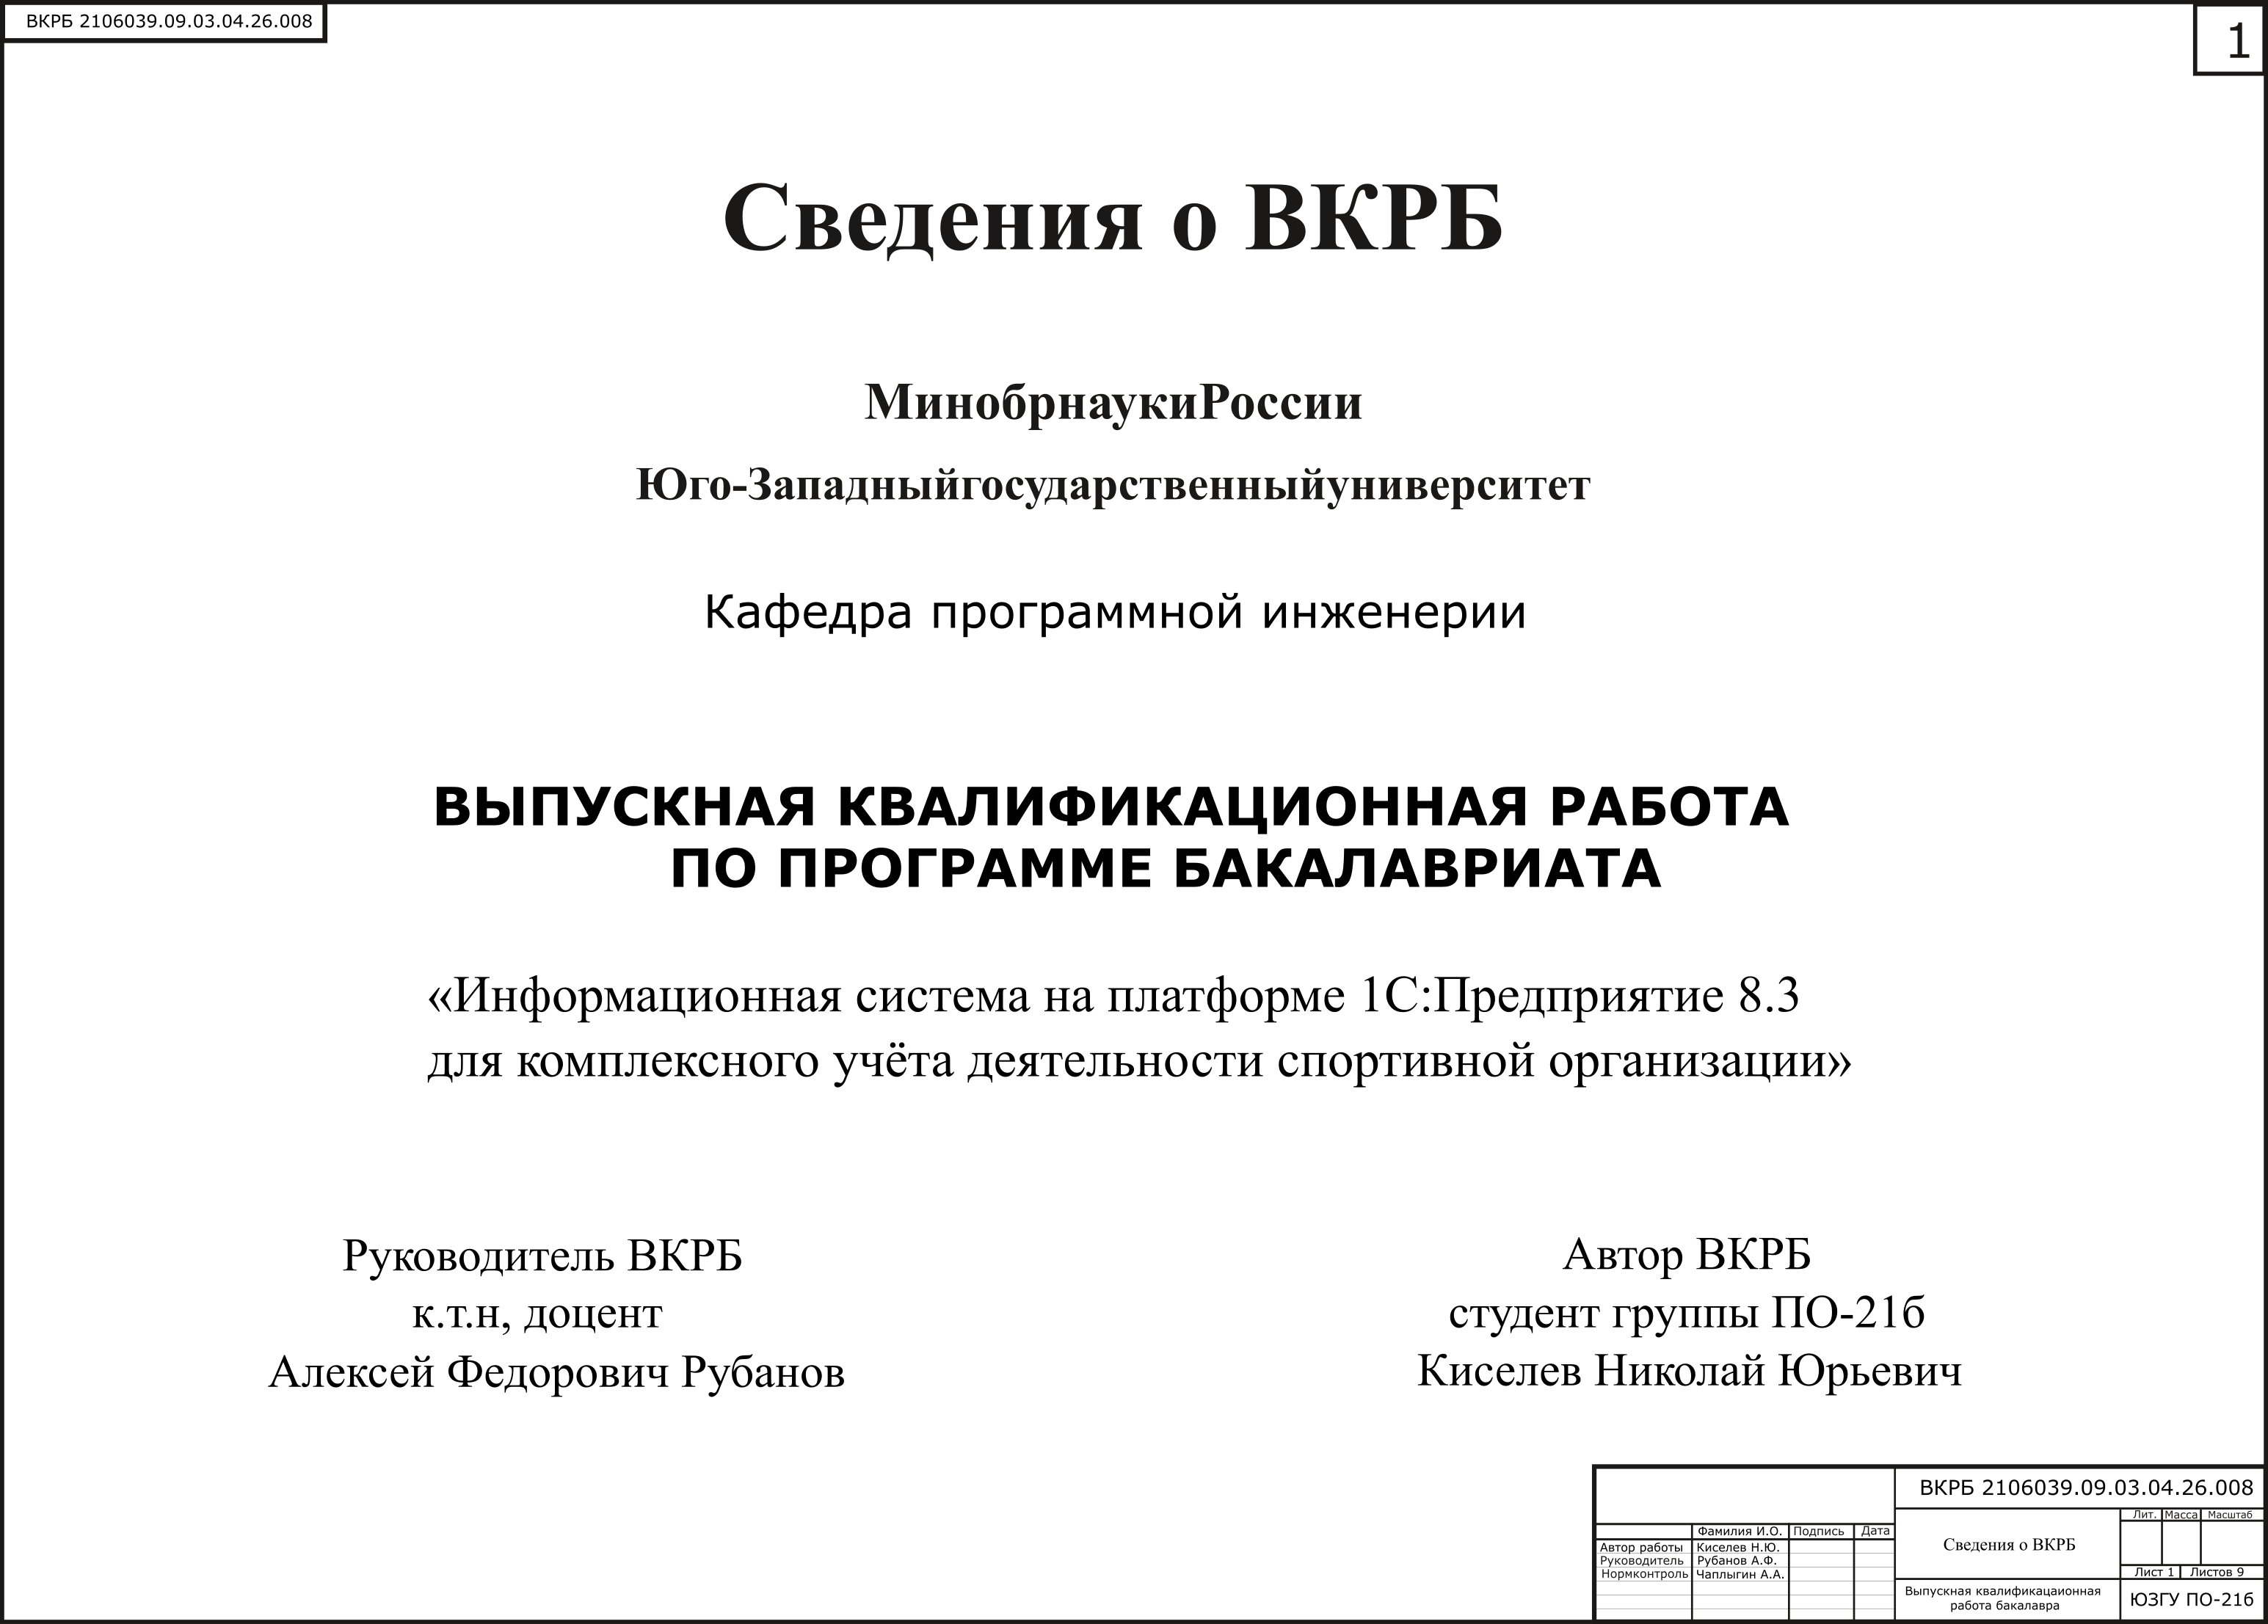
\includegraphics[width=0.85\linewidth]{images/Diplom1.png}
		\заголовок{Сведения о ВКРБ}
		\label{pl1:image}
	\end{плакат}
	
	
	\begin{плакат}
		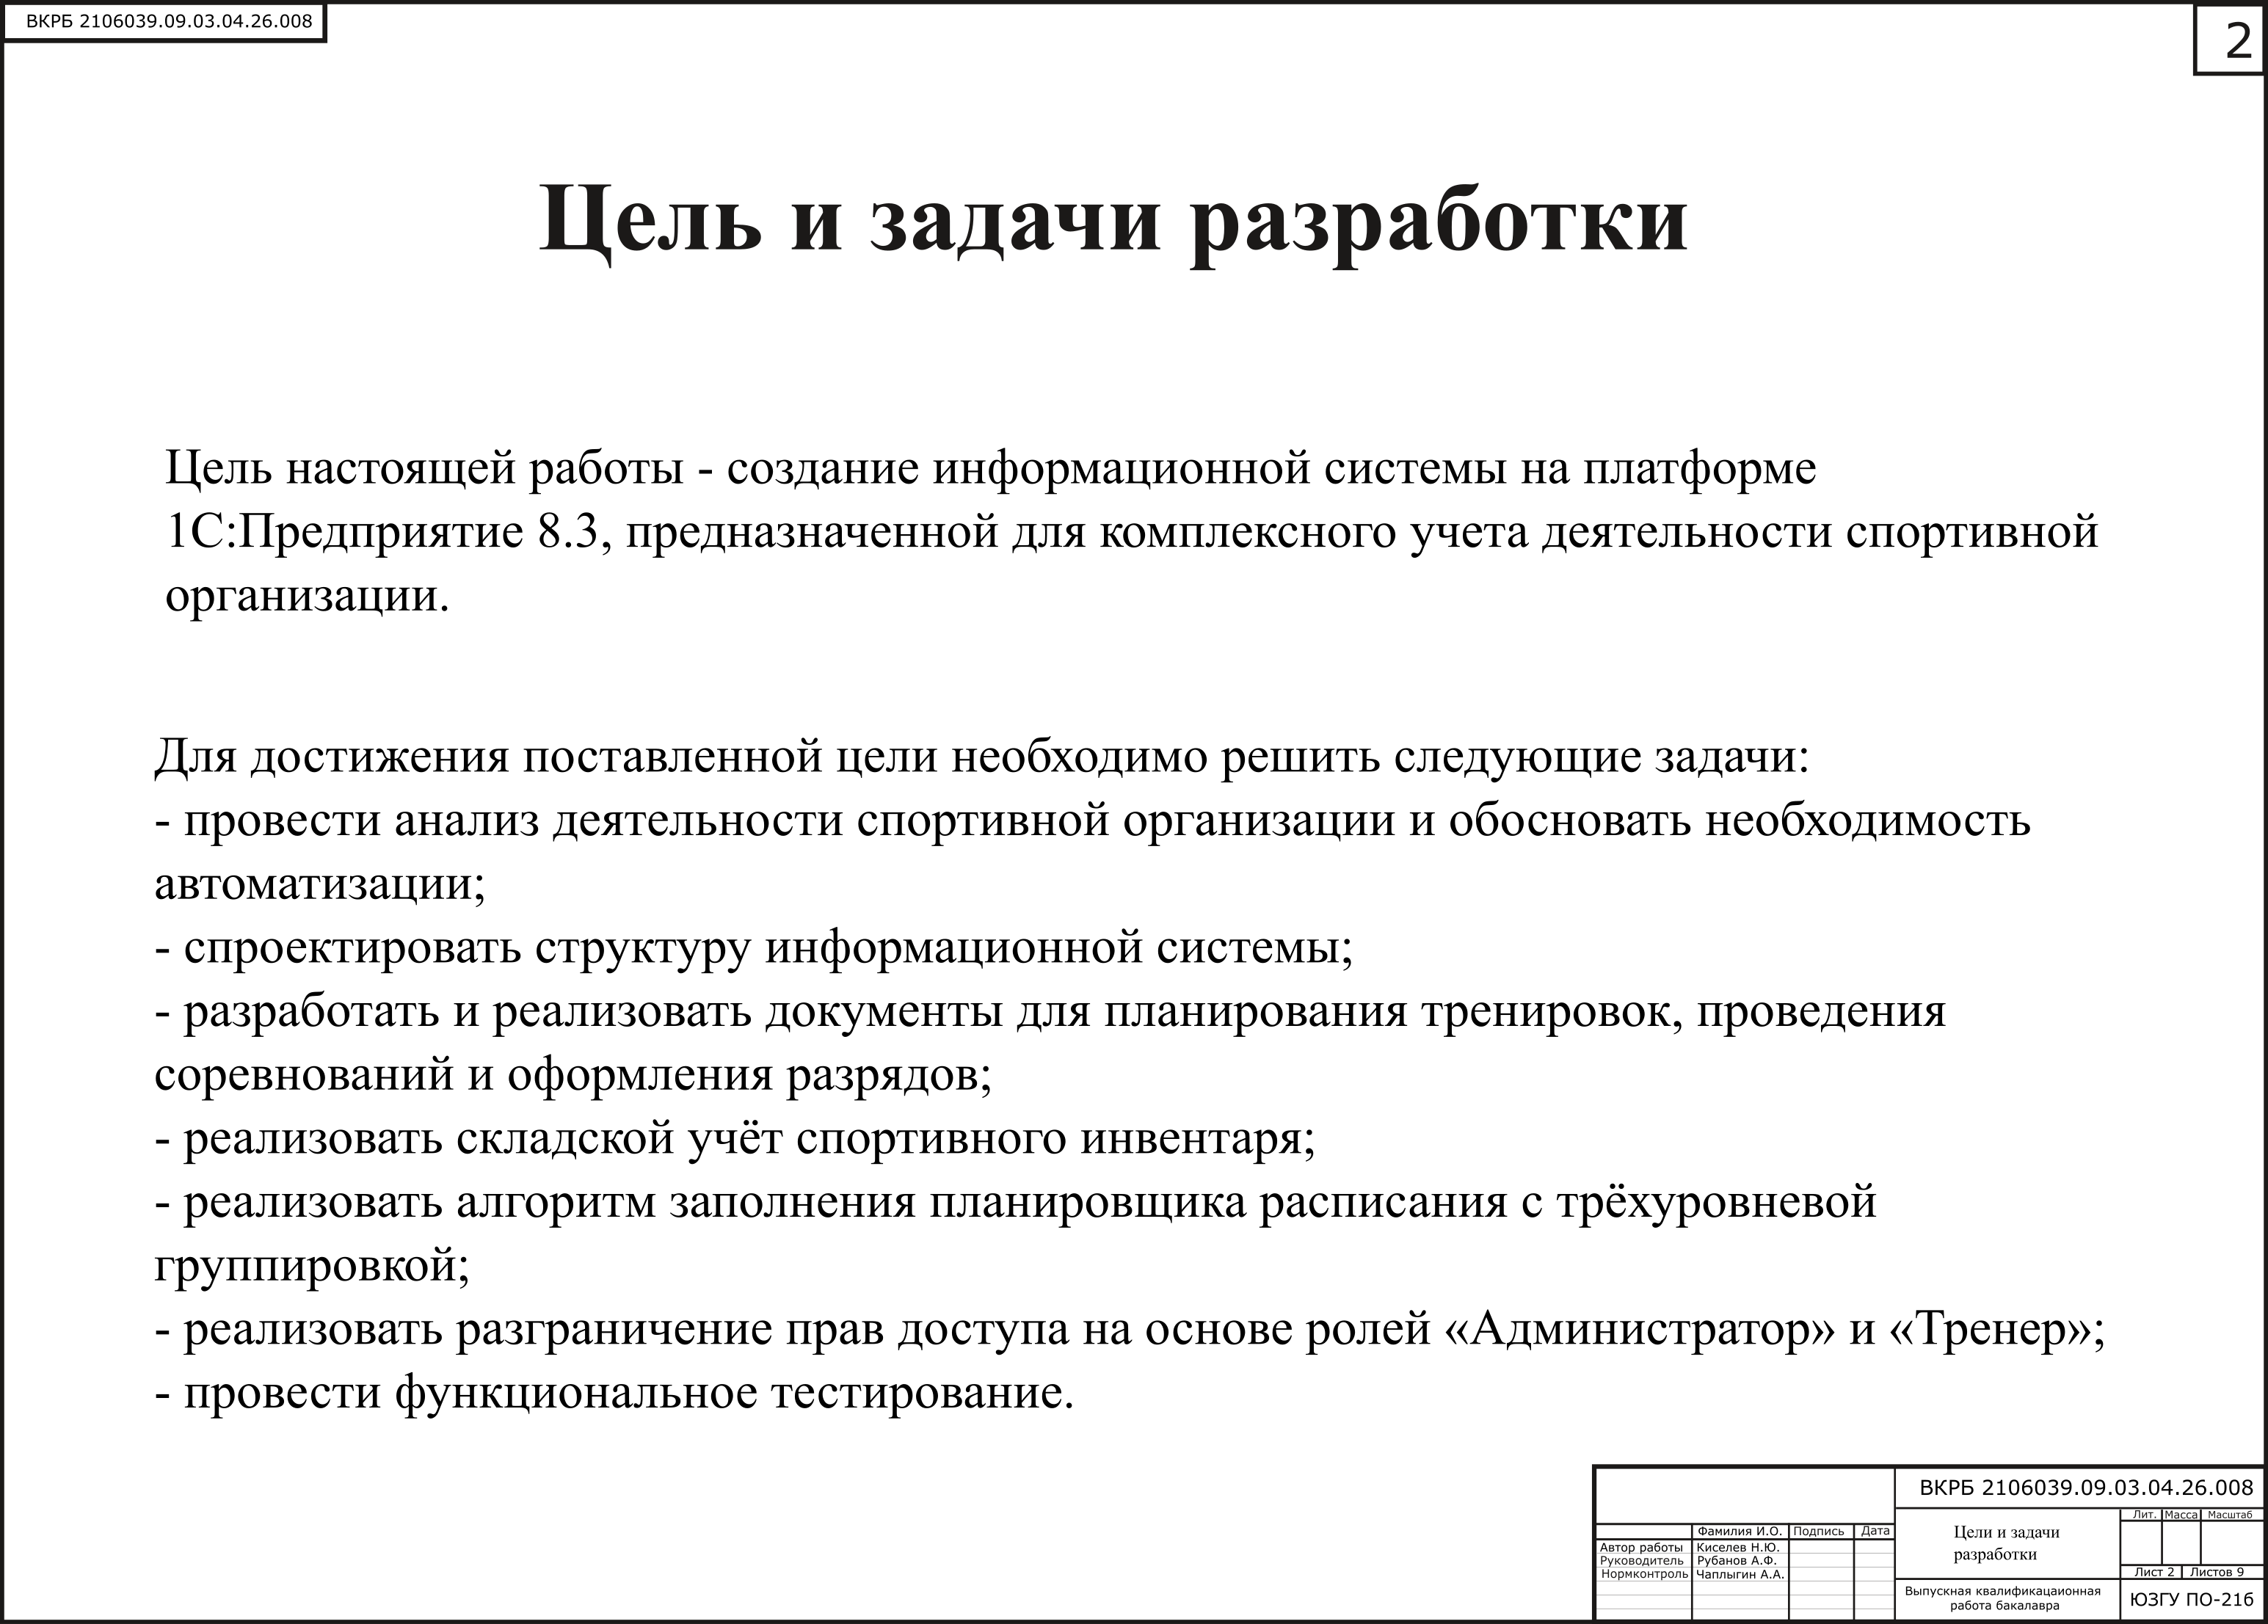
\includegraphics[width=0.85\linewidth]{images/Diplom2.png}
		\заголовок{Цель и задачи разработки}
		\label{pl2:image}      
	\end{плакат}
	
	\begin{плакат}
		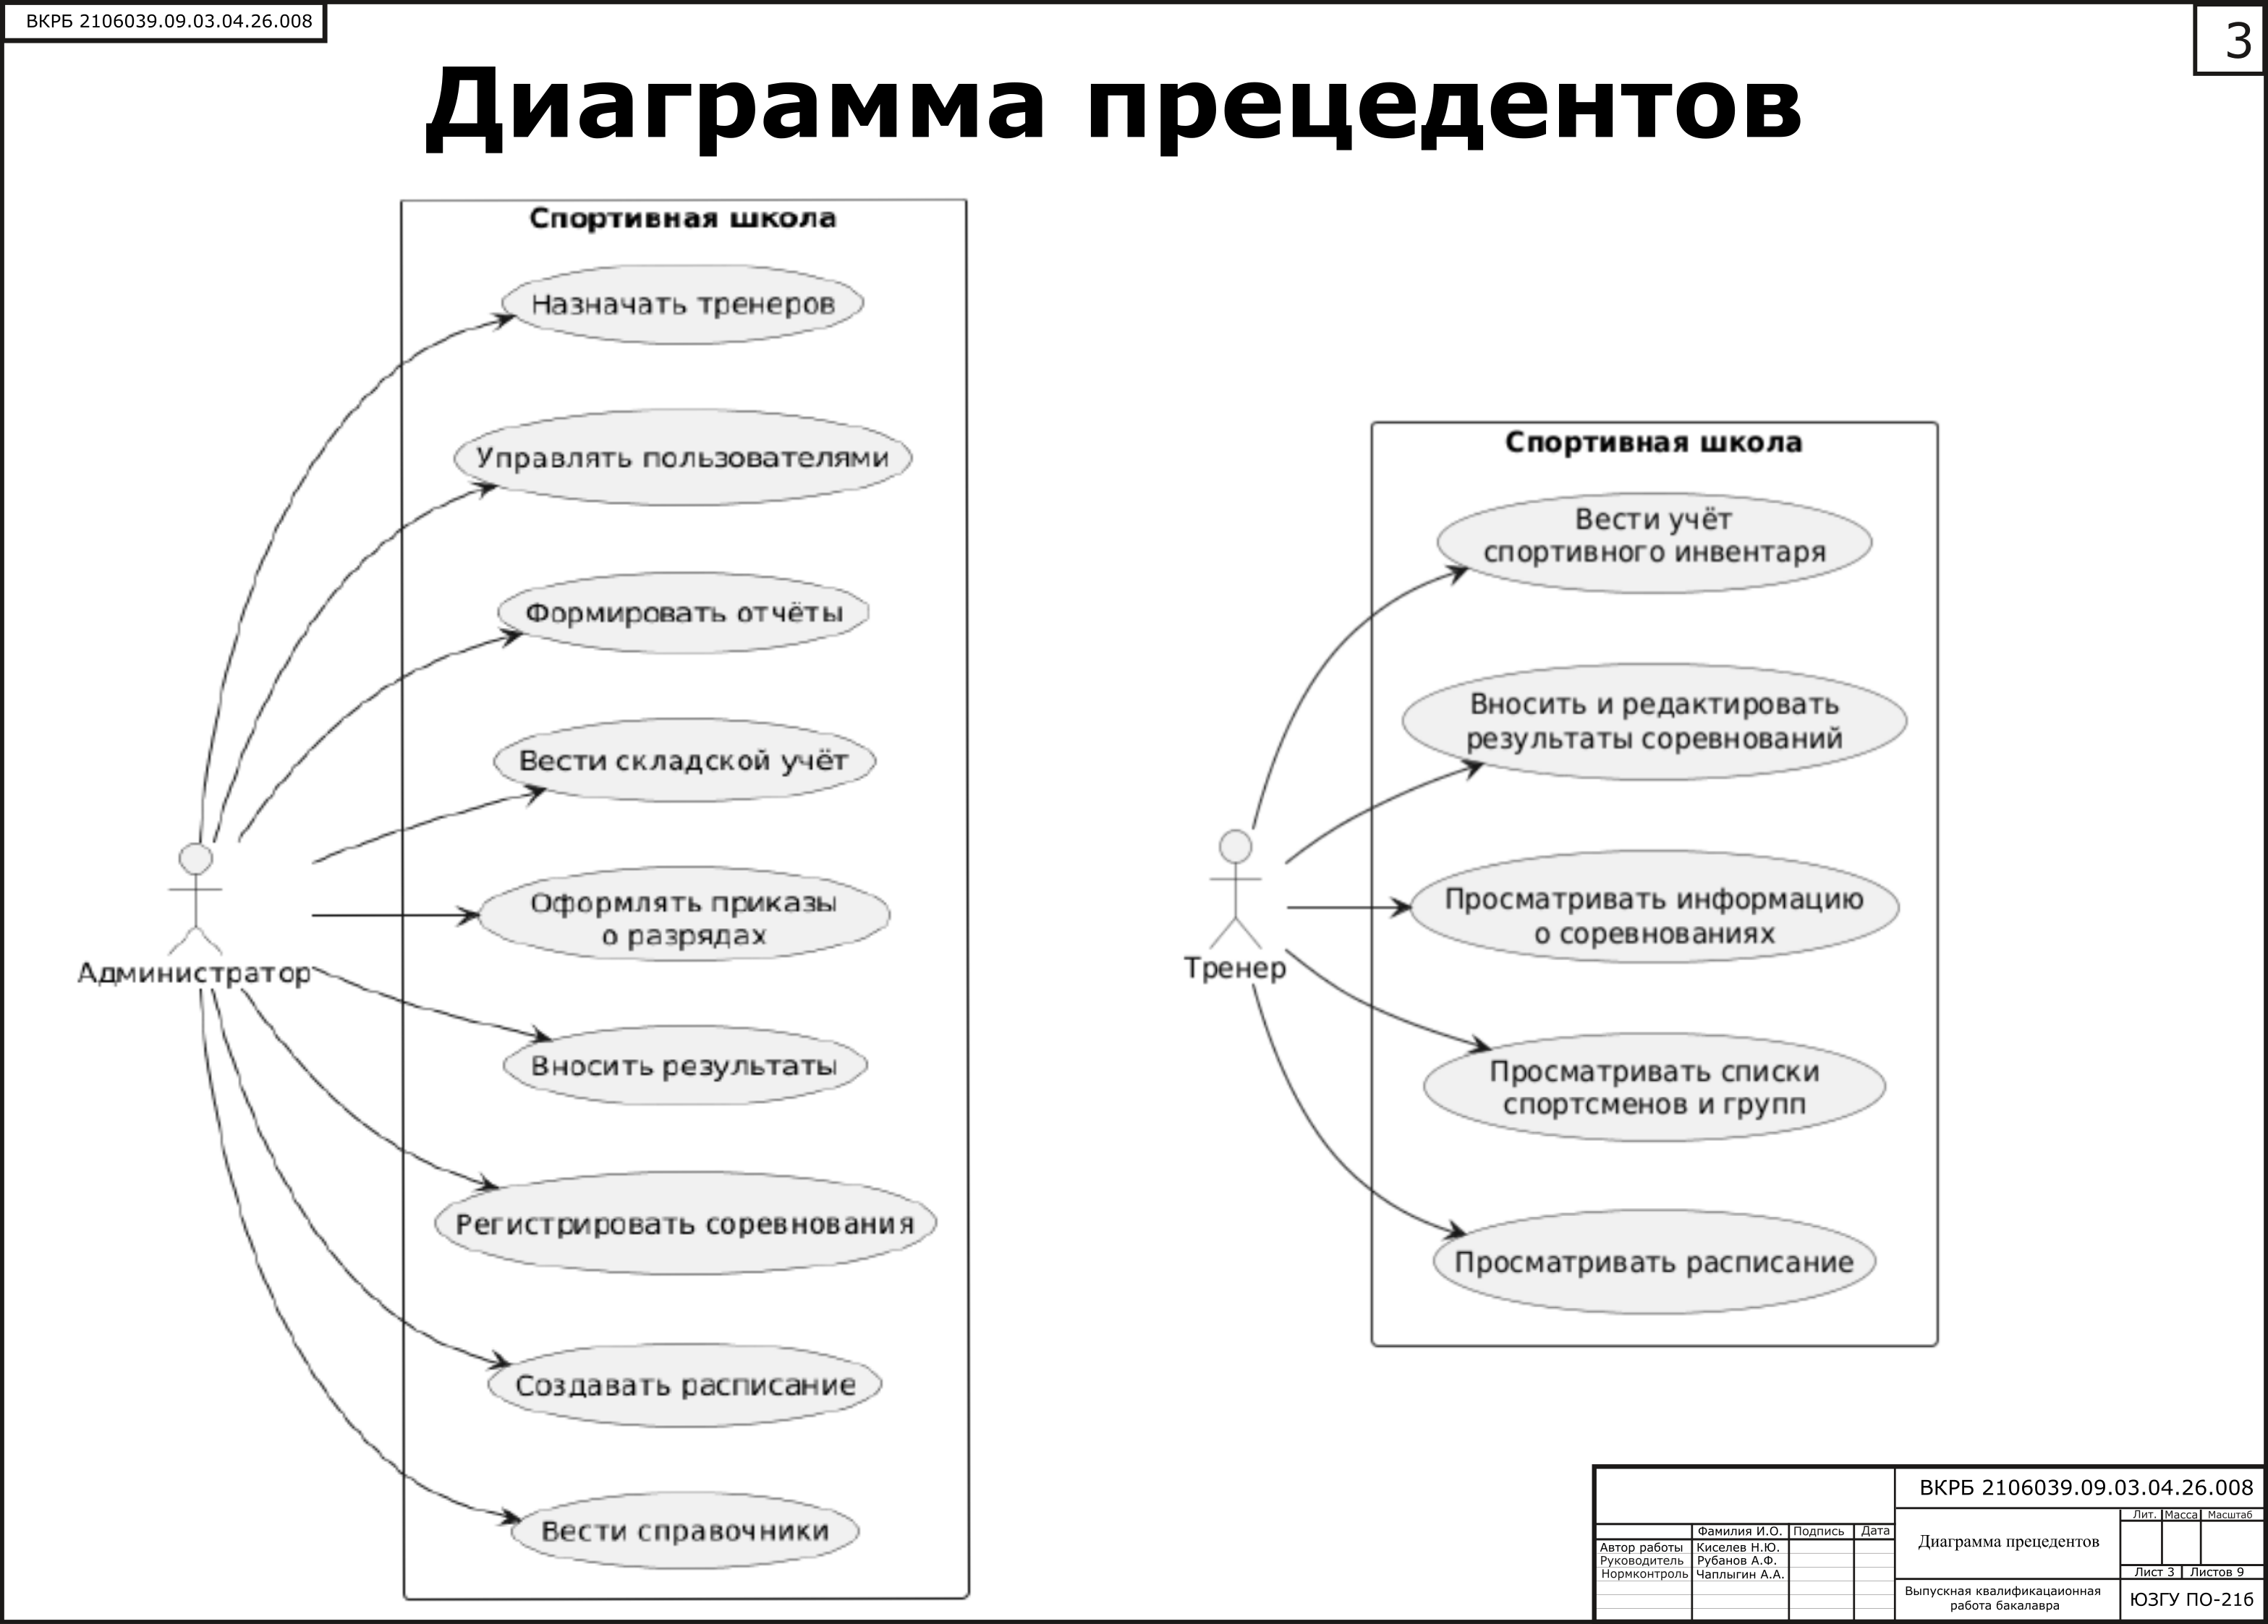
\includegraphics[width=0.85\linewidth]{images/Diplom3.png}
		\заголовок{Диаграмма прецедентов}
		\label{pl3:image}      
	\end{плакат}
	
	\begin{плакат}
		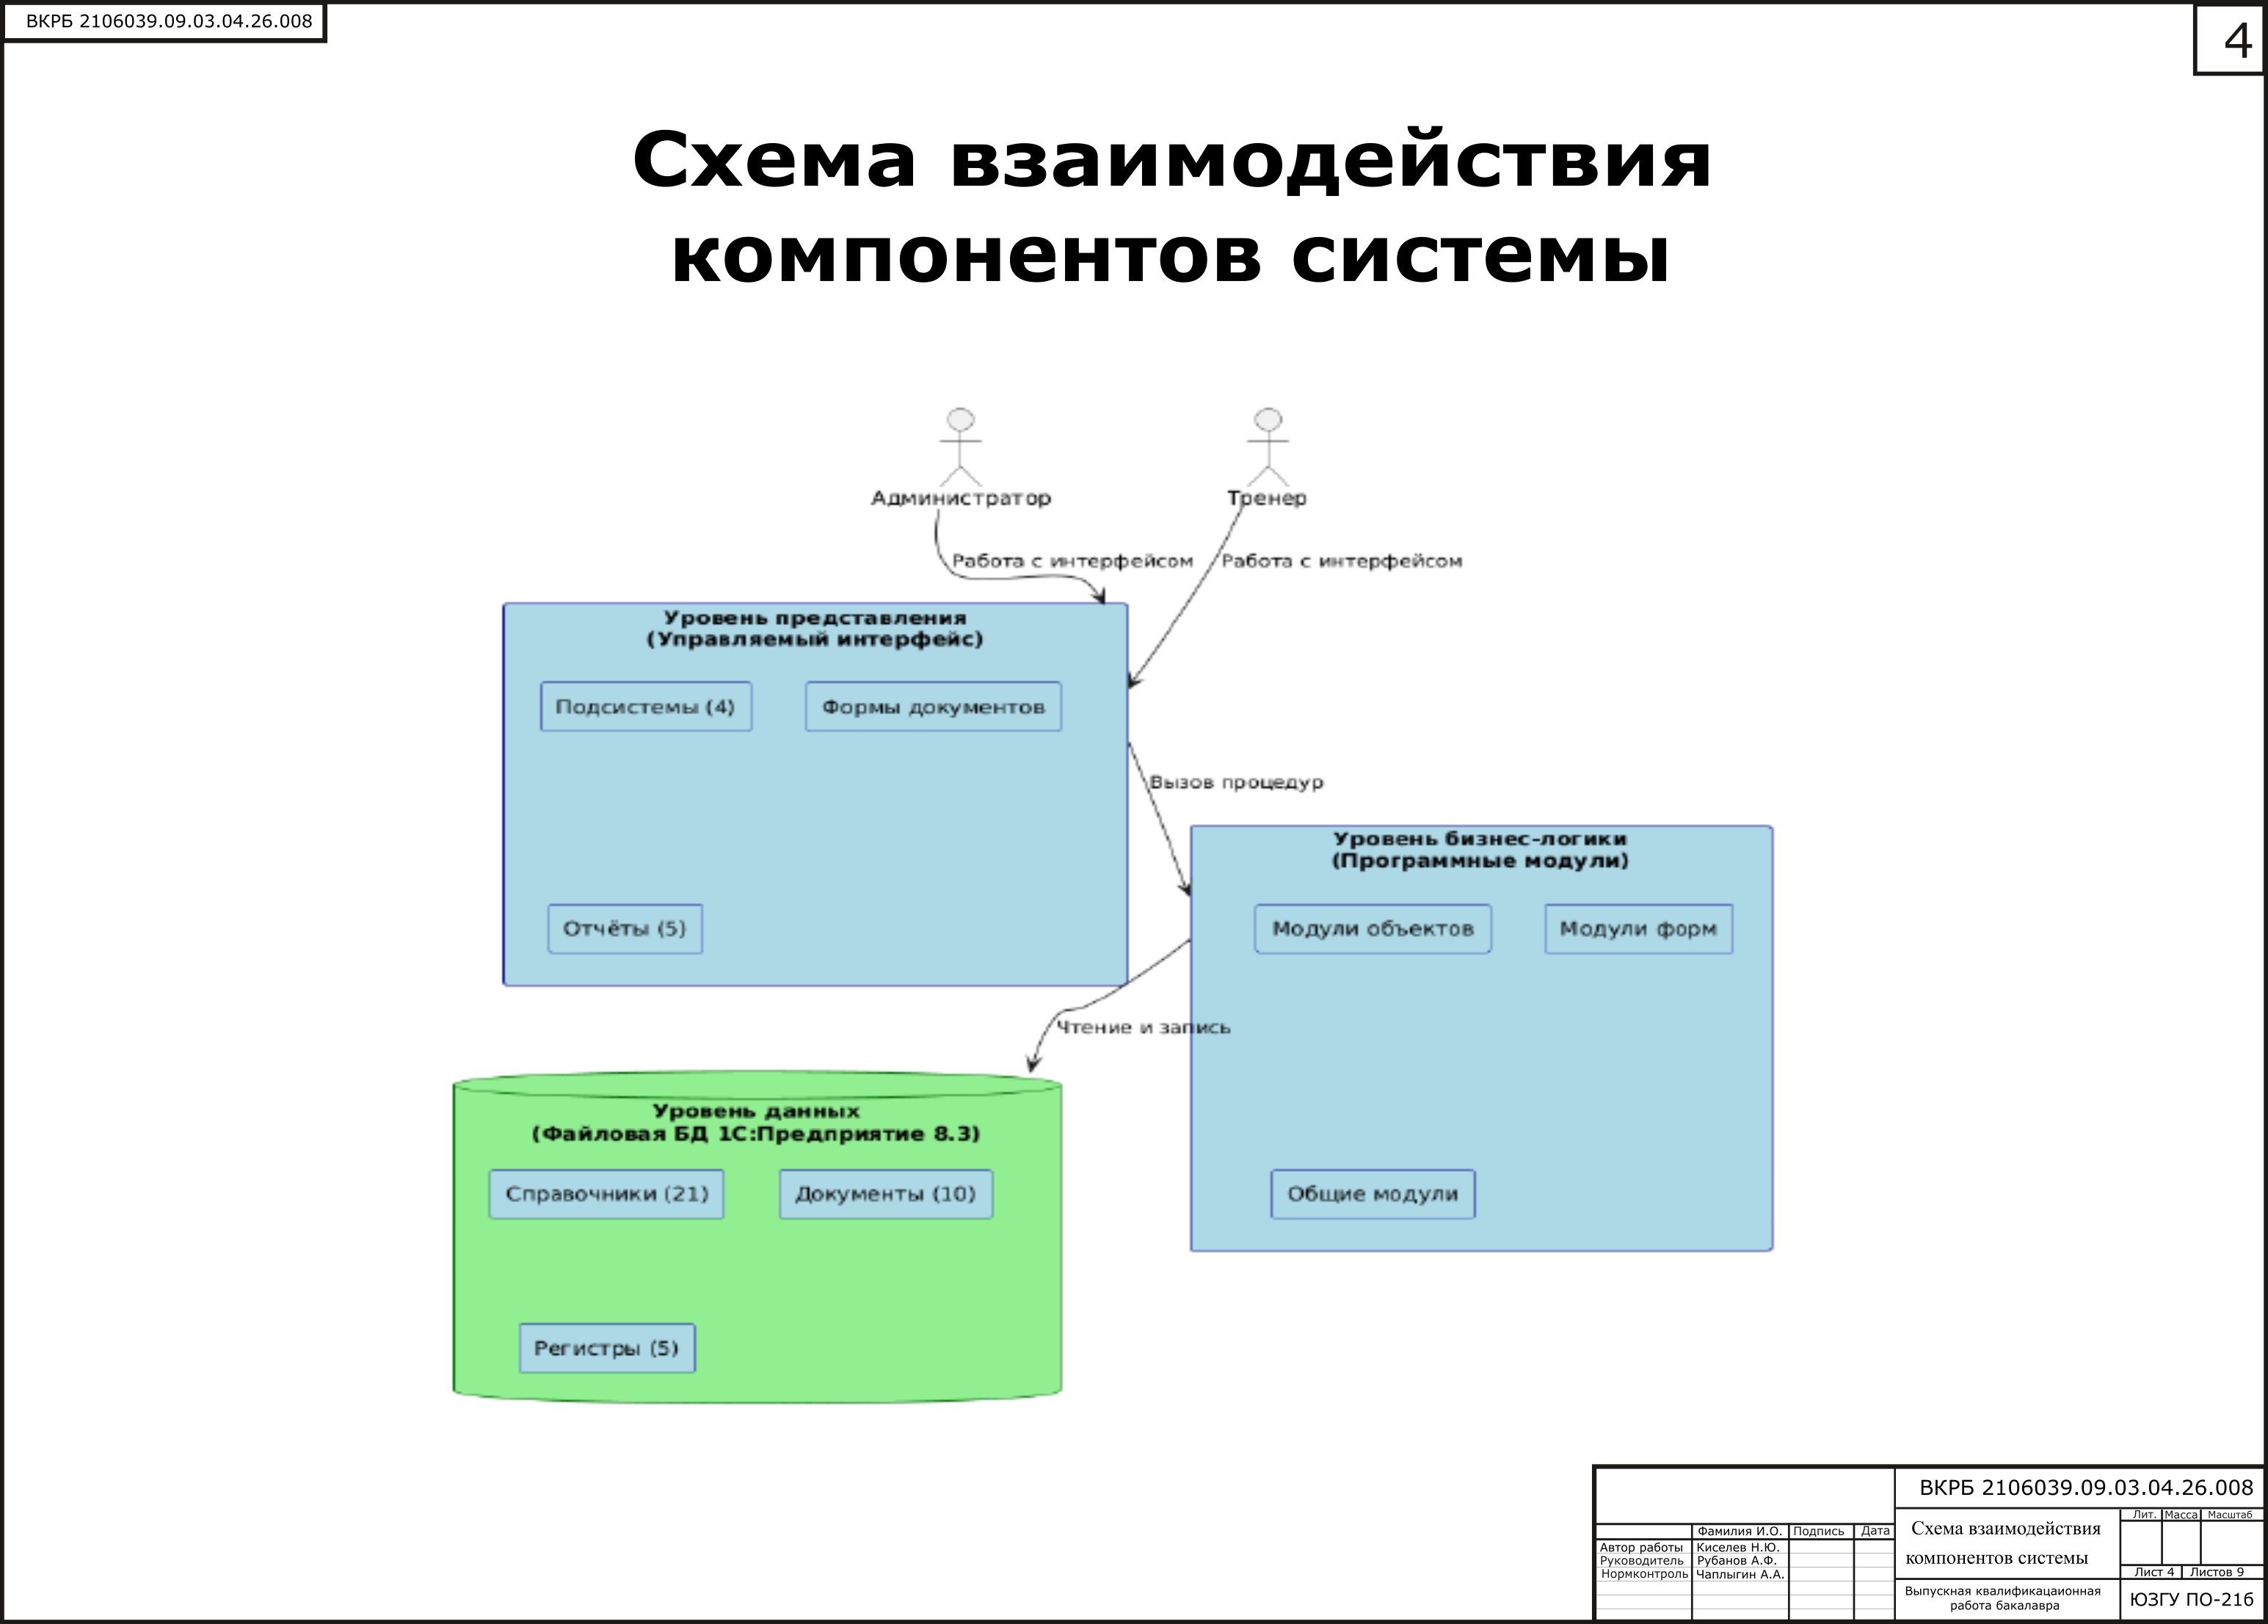
\includegraphics[width=0.85\linewidth]{images/Diplom4.png}
		\заголовок{Схема взаимодействия компонентов системы}
		\label{pl4:image}      
	\end{плакат}
	
	\begin{плакат}
		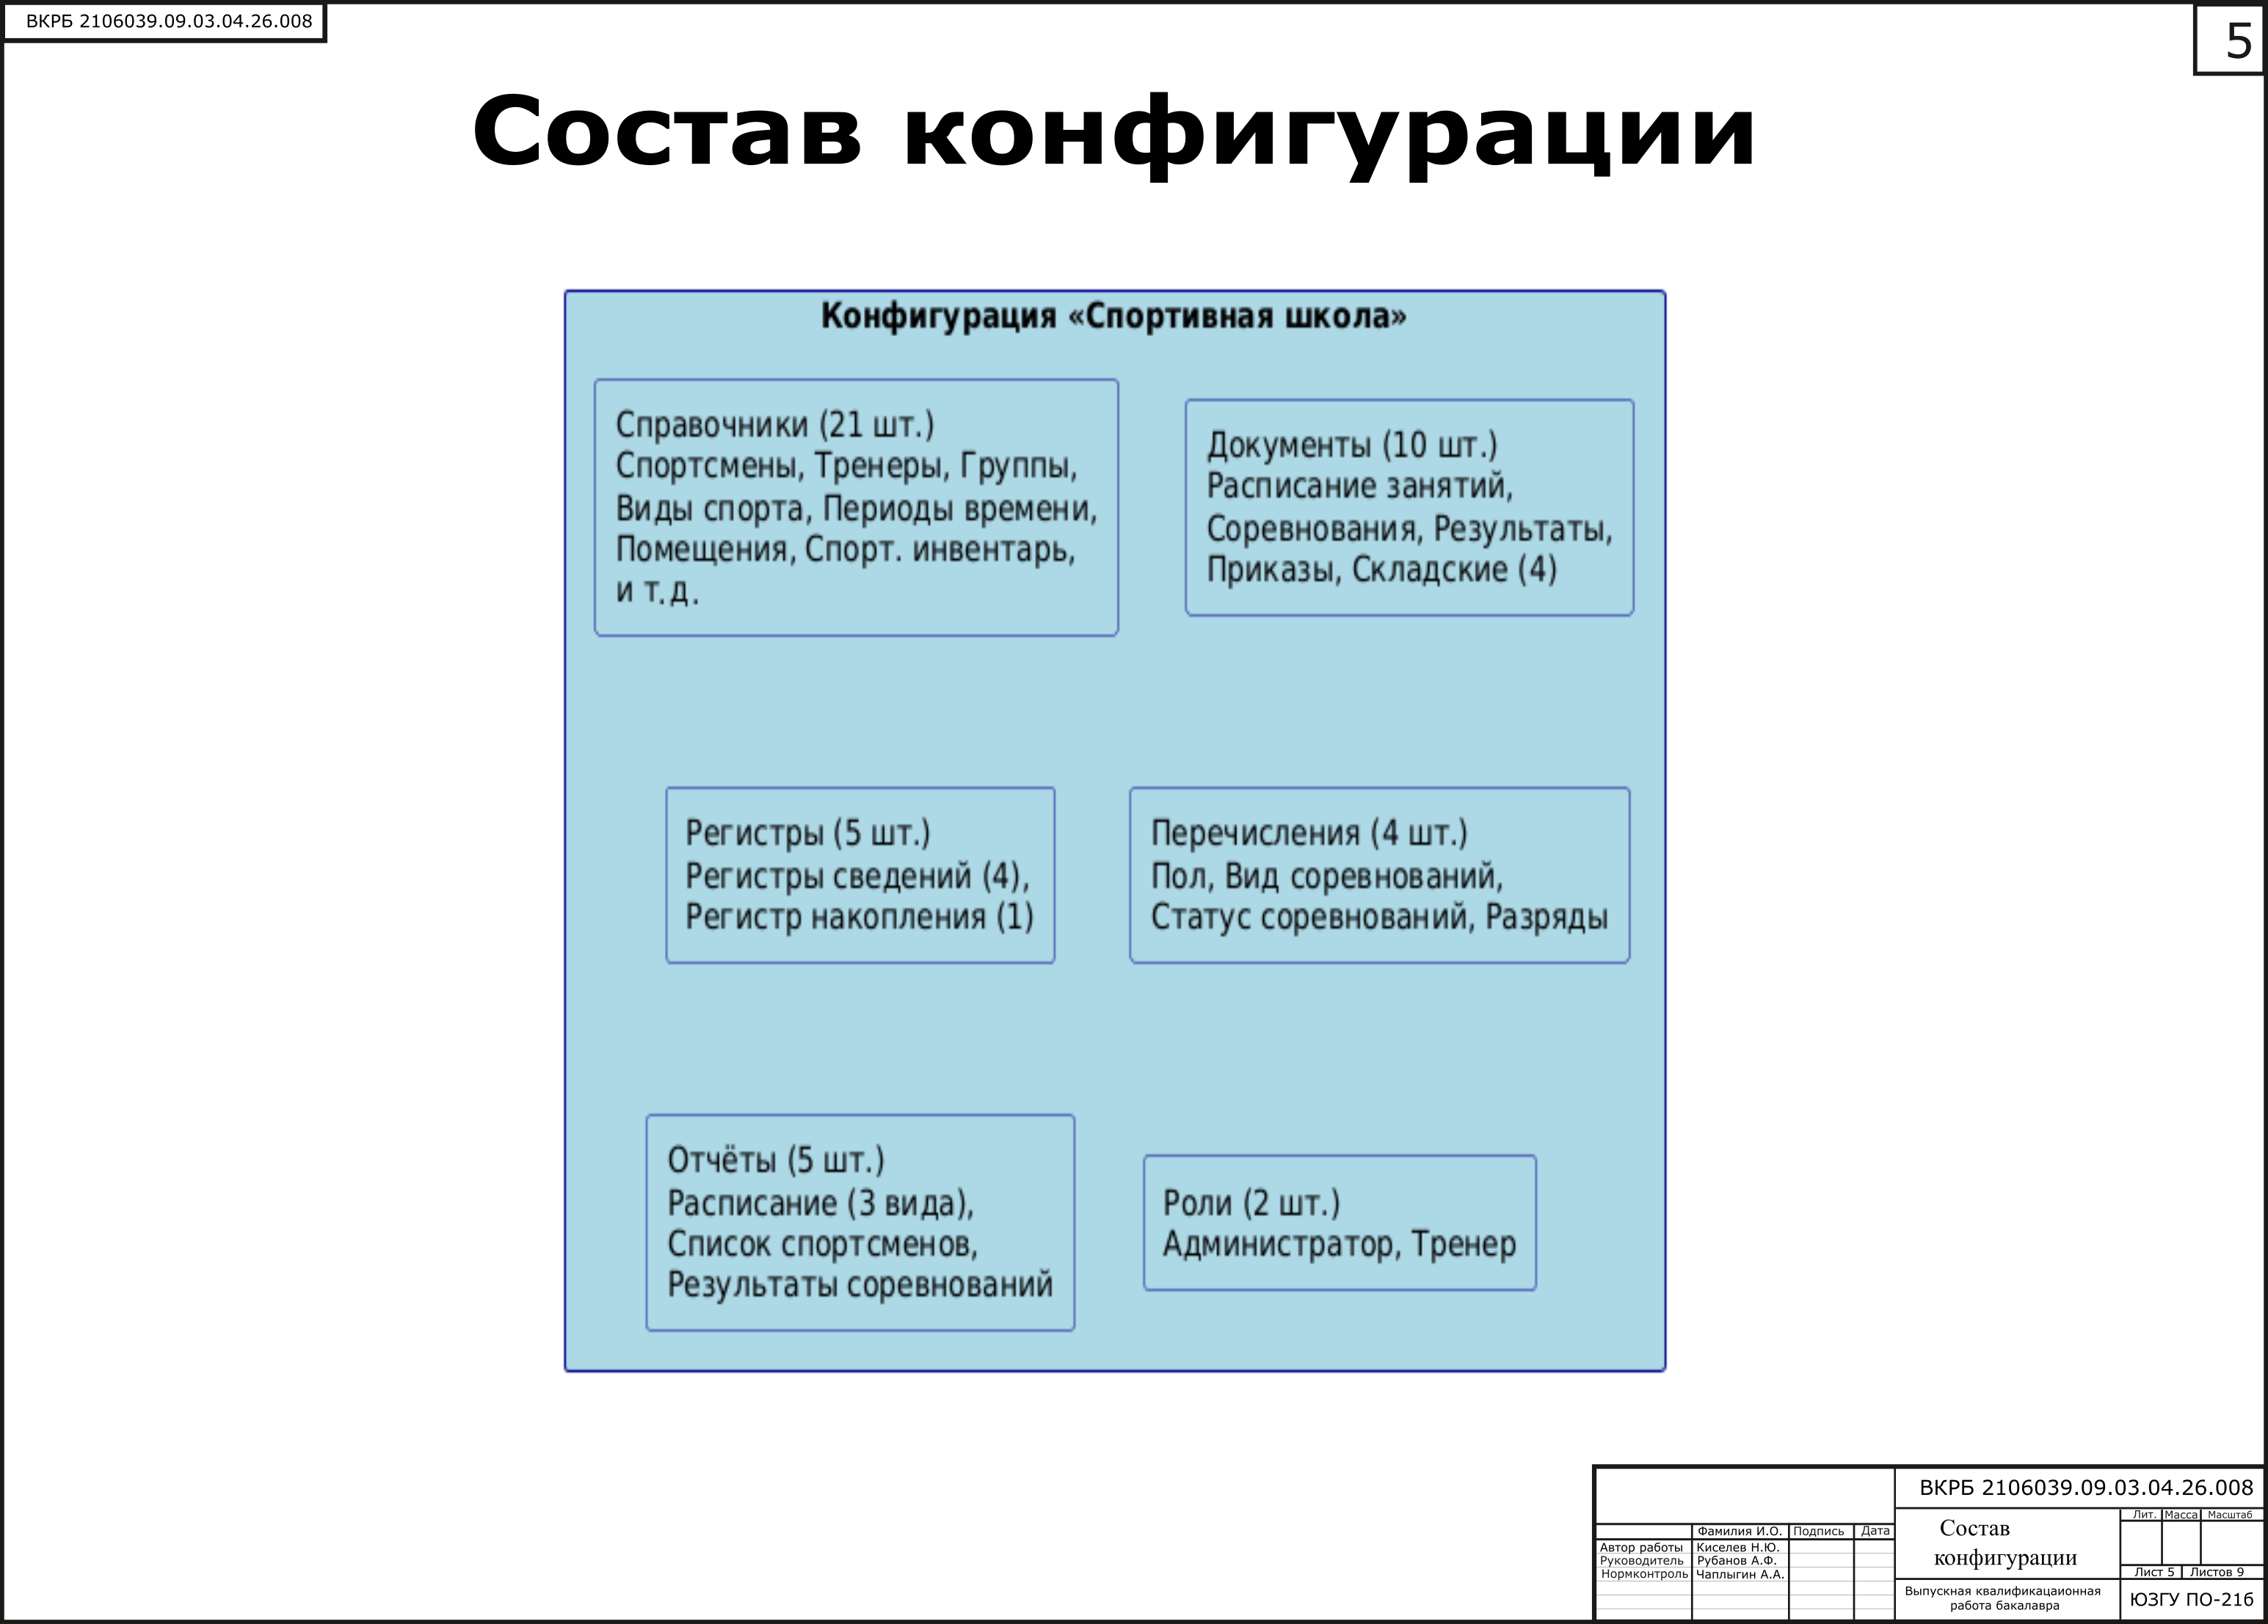
\includegraphics[width=0.85\linewidth]{images/Diplom5.png}
		\заголовок{Состав конфигурации}
		\label{pl5:image}      
	\end{плакат}
	
	\begin{плакат}
		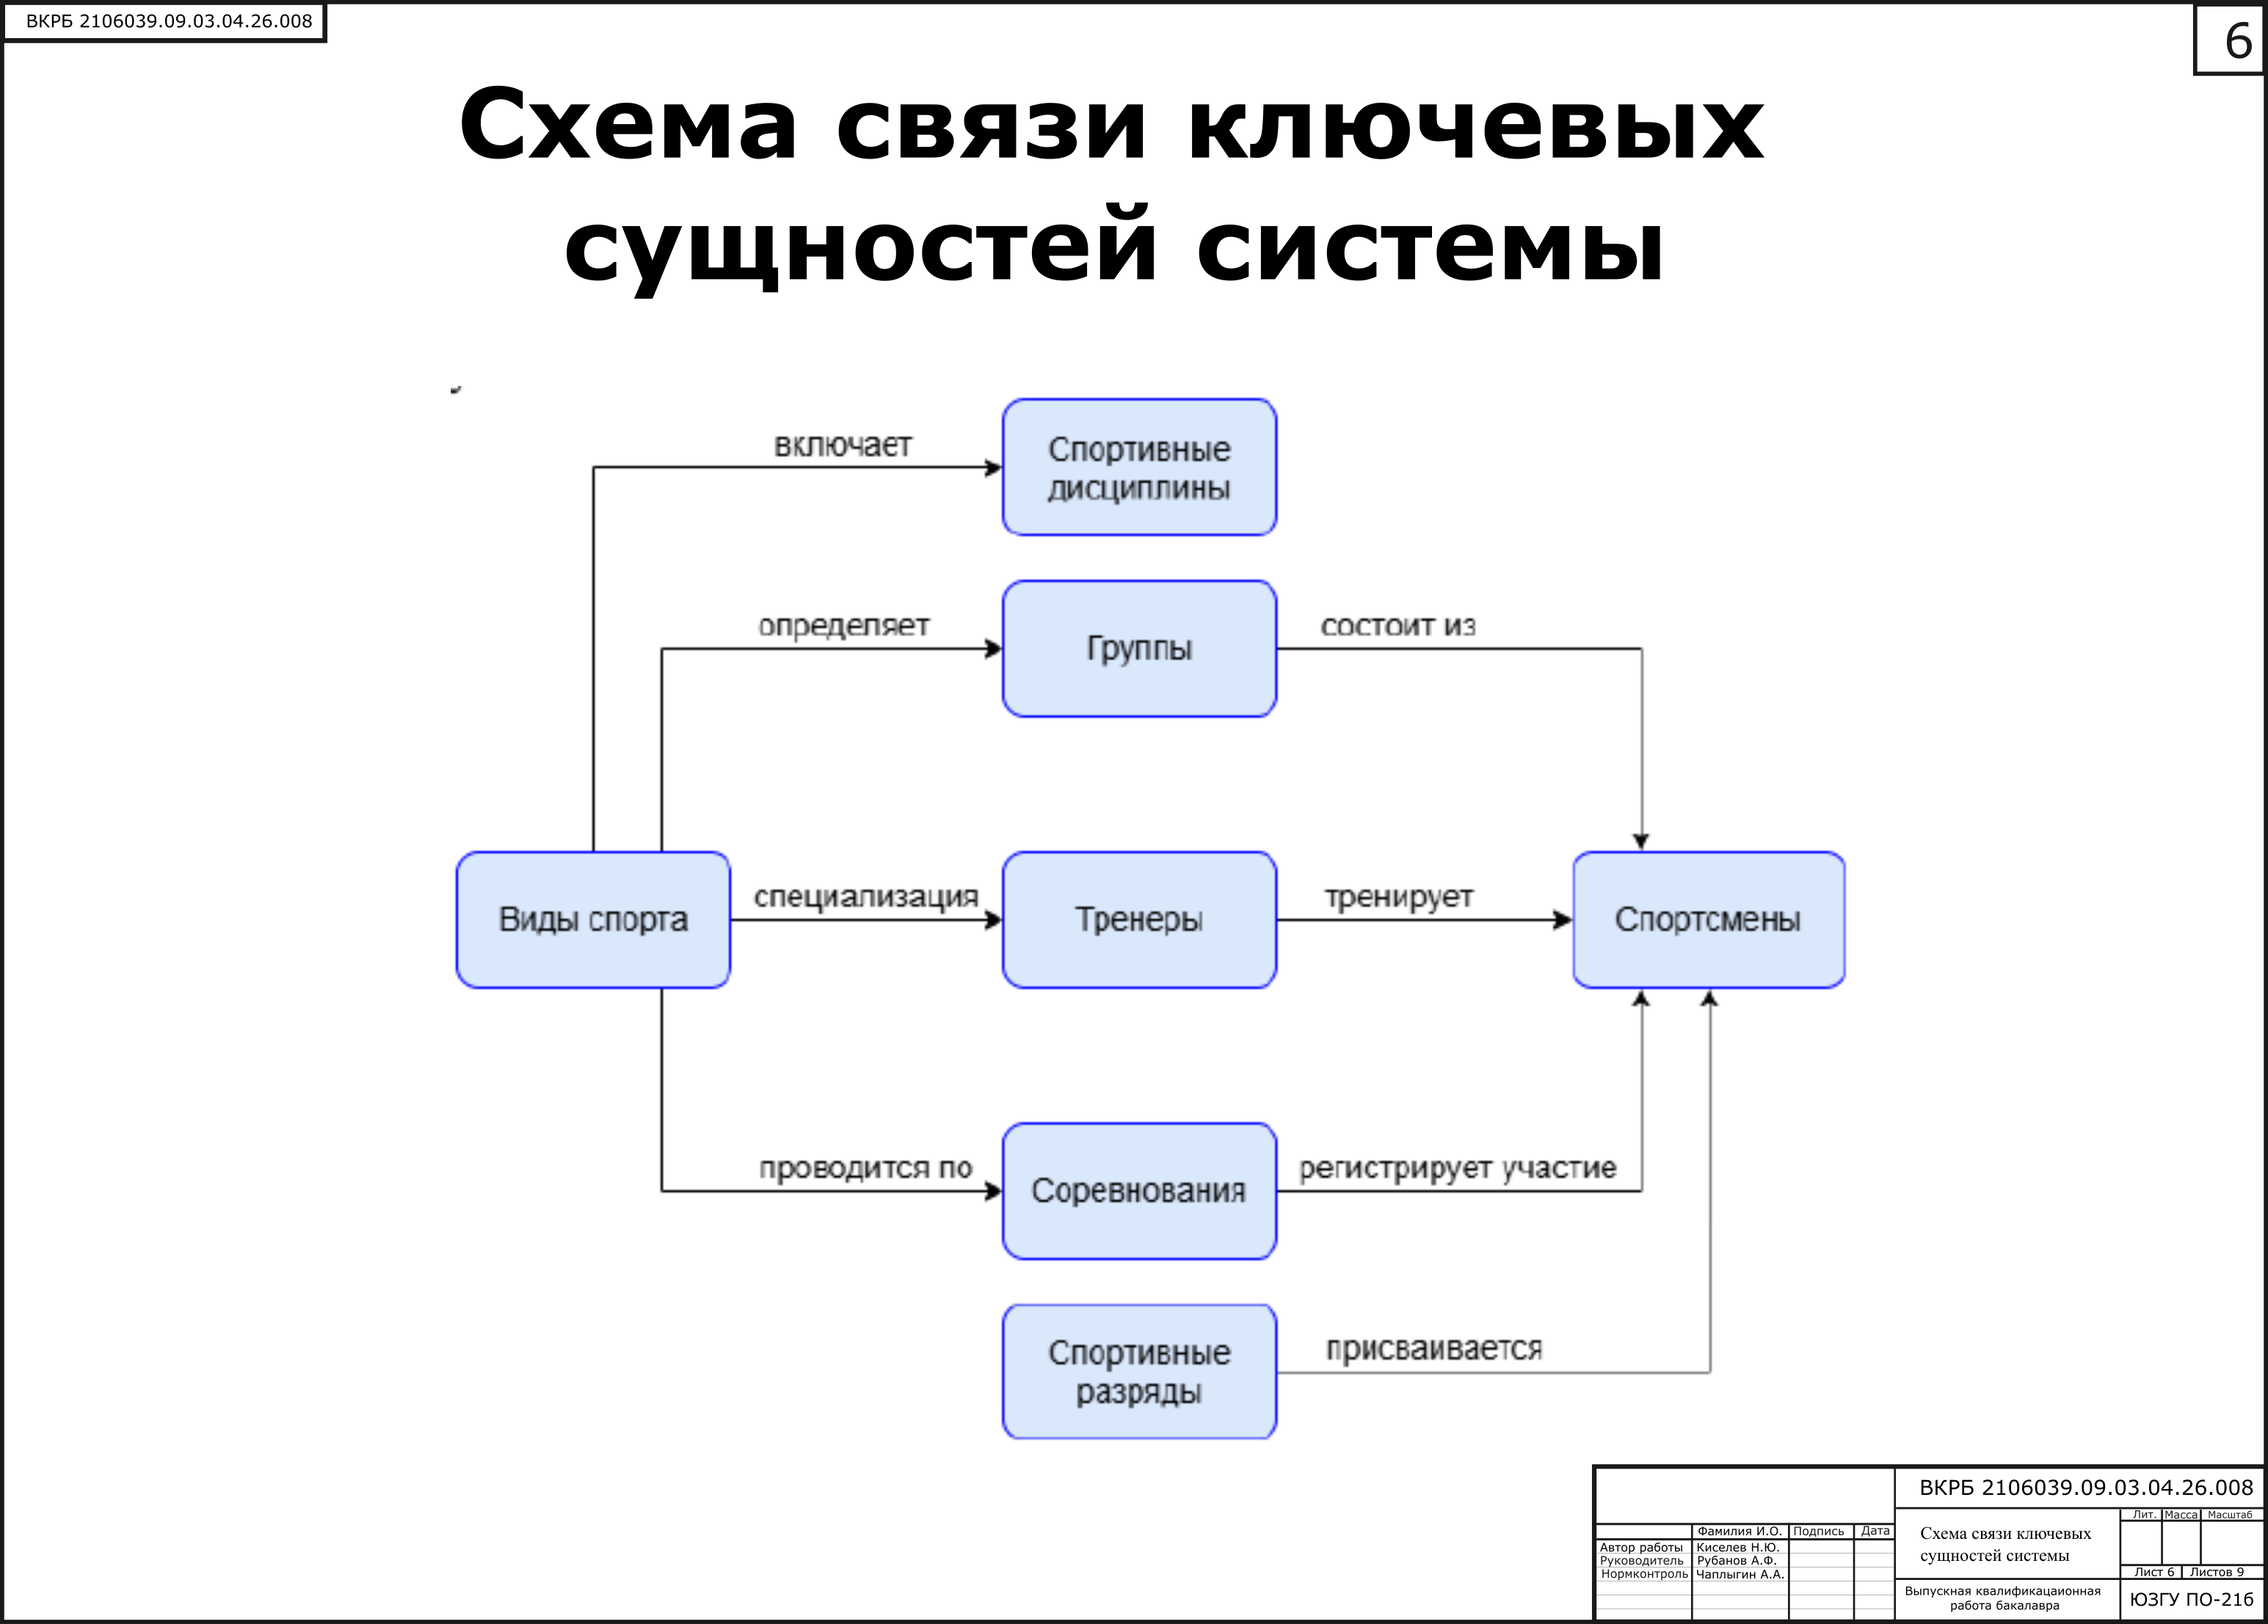
\includegraphics[width=0.85\linewidth]{images/Diplom6.png}
		\заголовок{Схема связи ключевых сущностей системы}
		\label{pl6:image}      
	\end{плакат}
	
	\begin{плакат}
		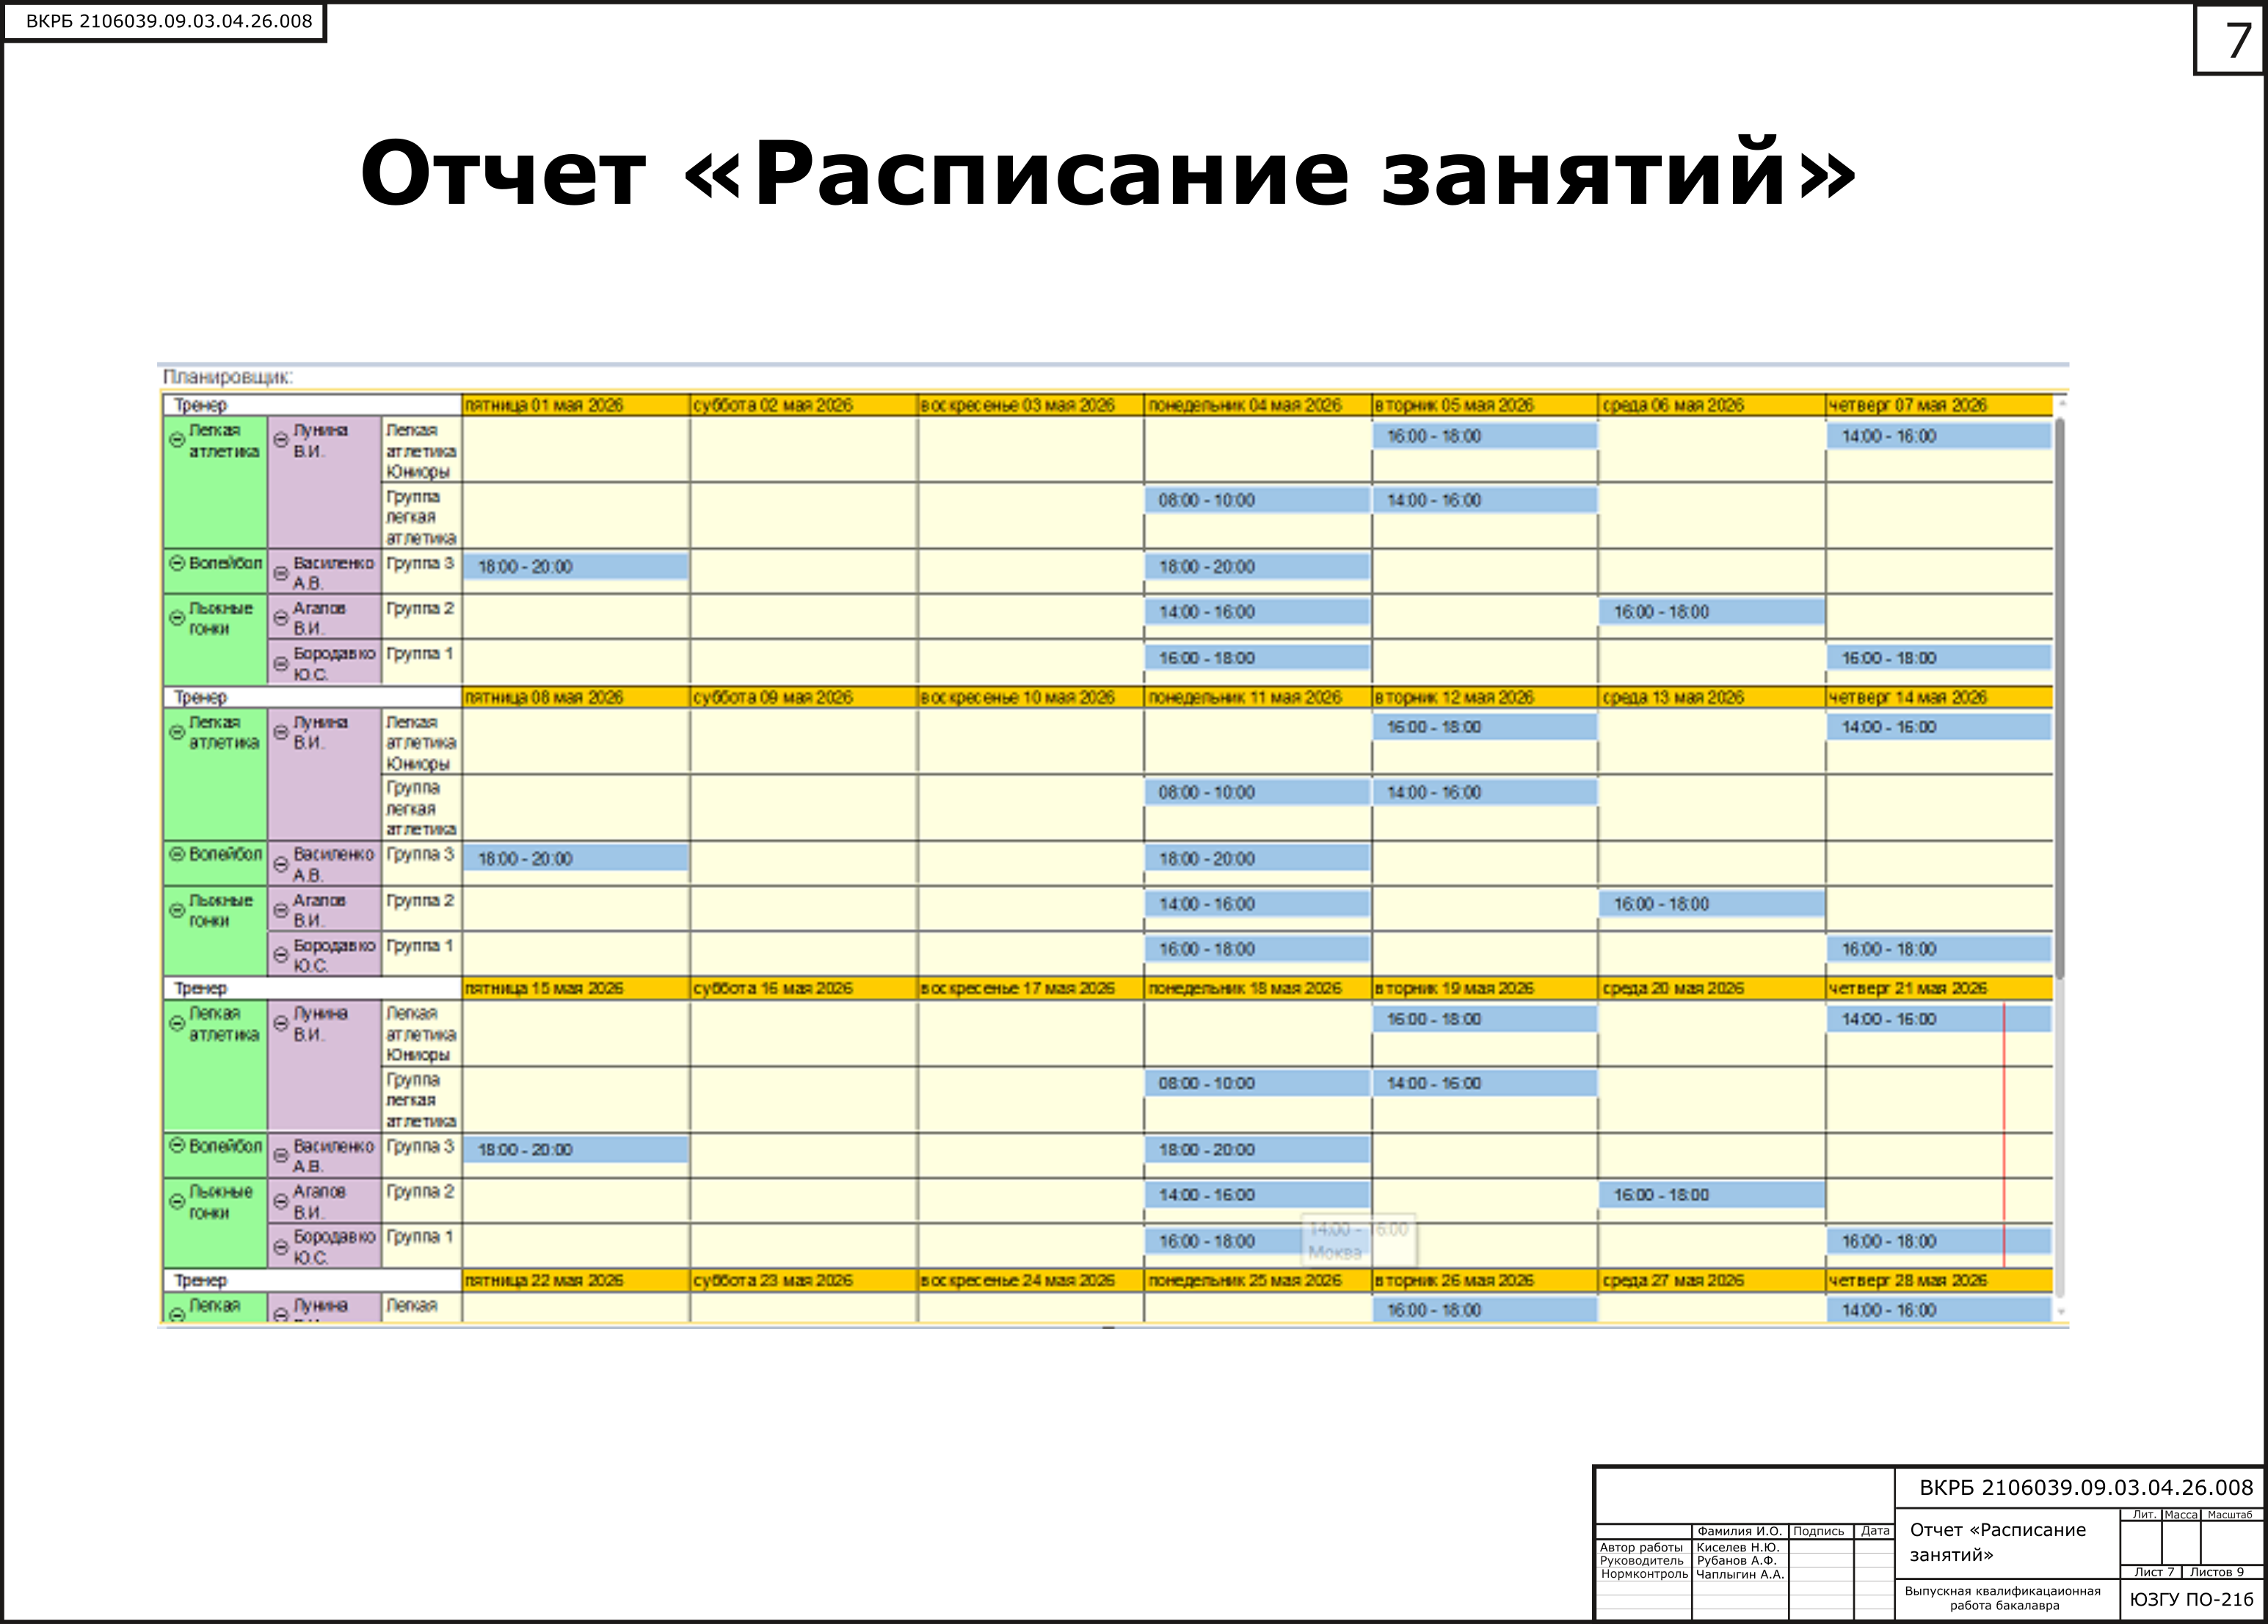
\includegraphics[width=0.85\linewidth]{images/Diplom7.png}
		\заголовок{Отчет «Расписание занятий»}
		\label{pl7:image}      
	\end{плакат}
	
	\begin{плакат}
		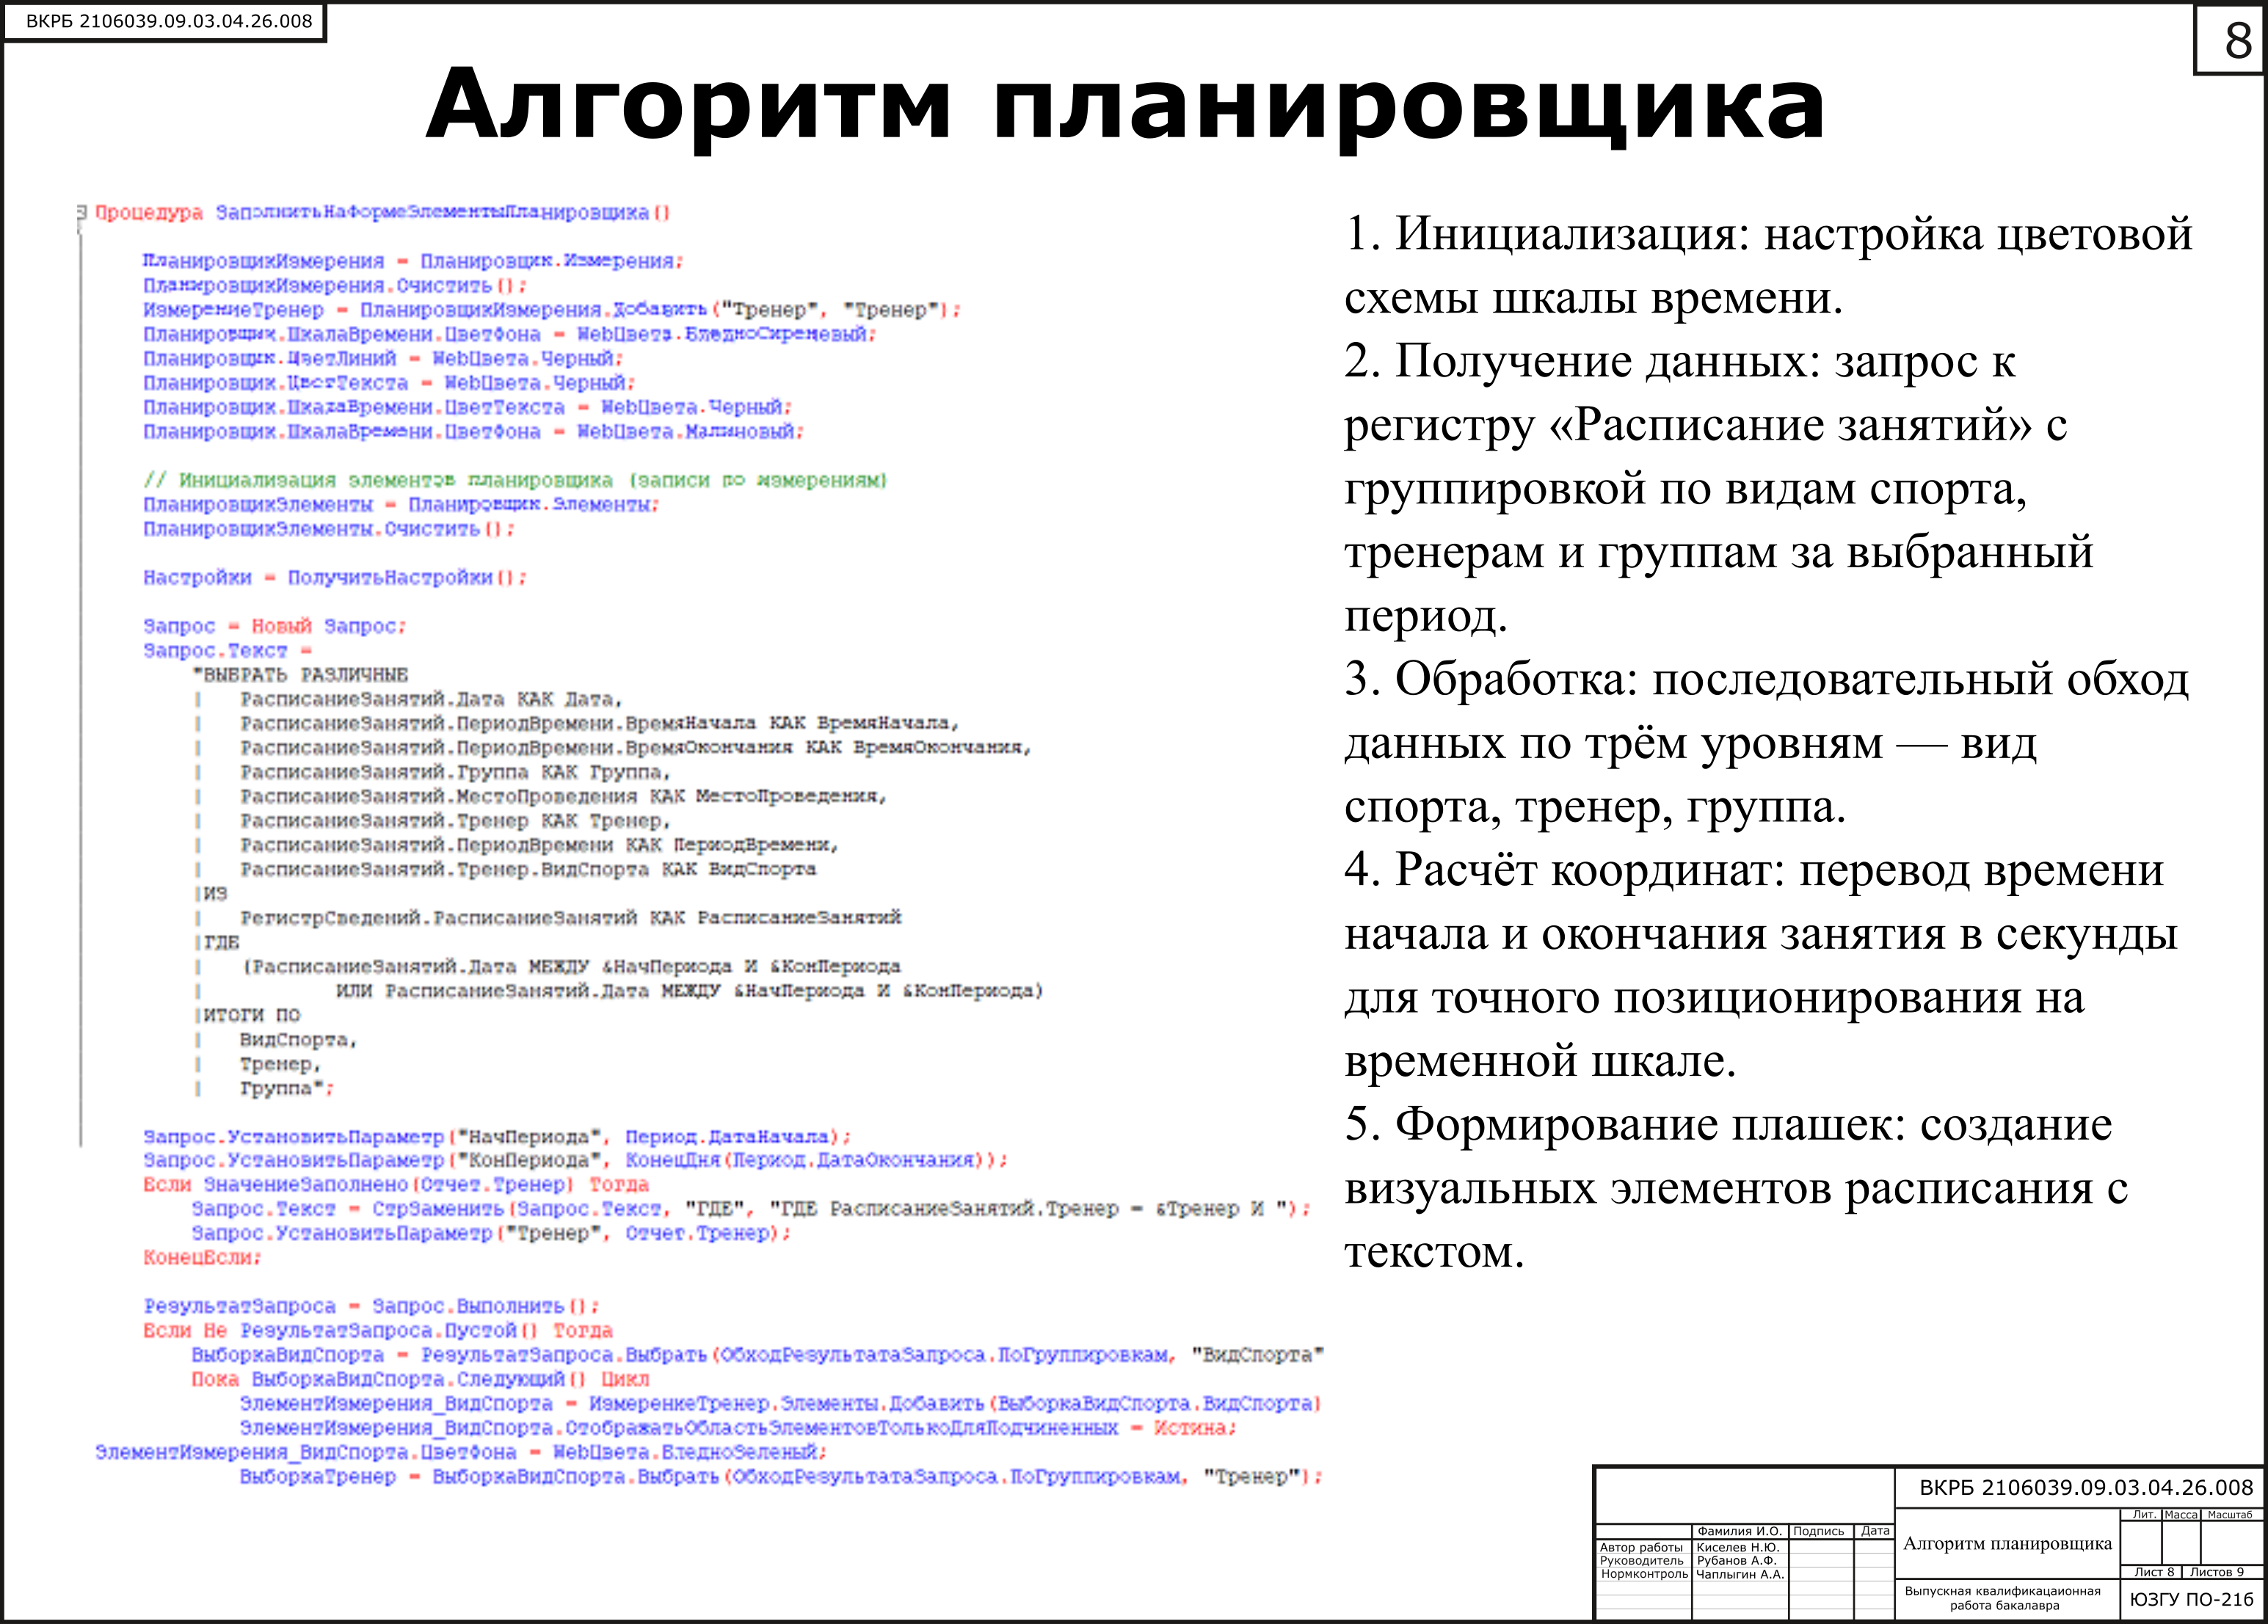
\includegraphics[width=0.85\linewidth]{images/Diplom8.png}
		\заголовок{Алгоритм планировщика}
		\label{pl8:image}      
	\end{плакат}
	
	\begin{плакат}
		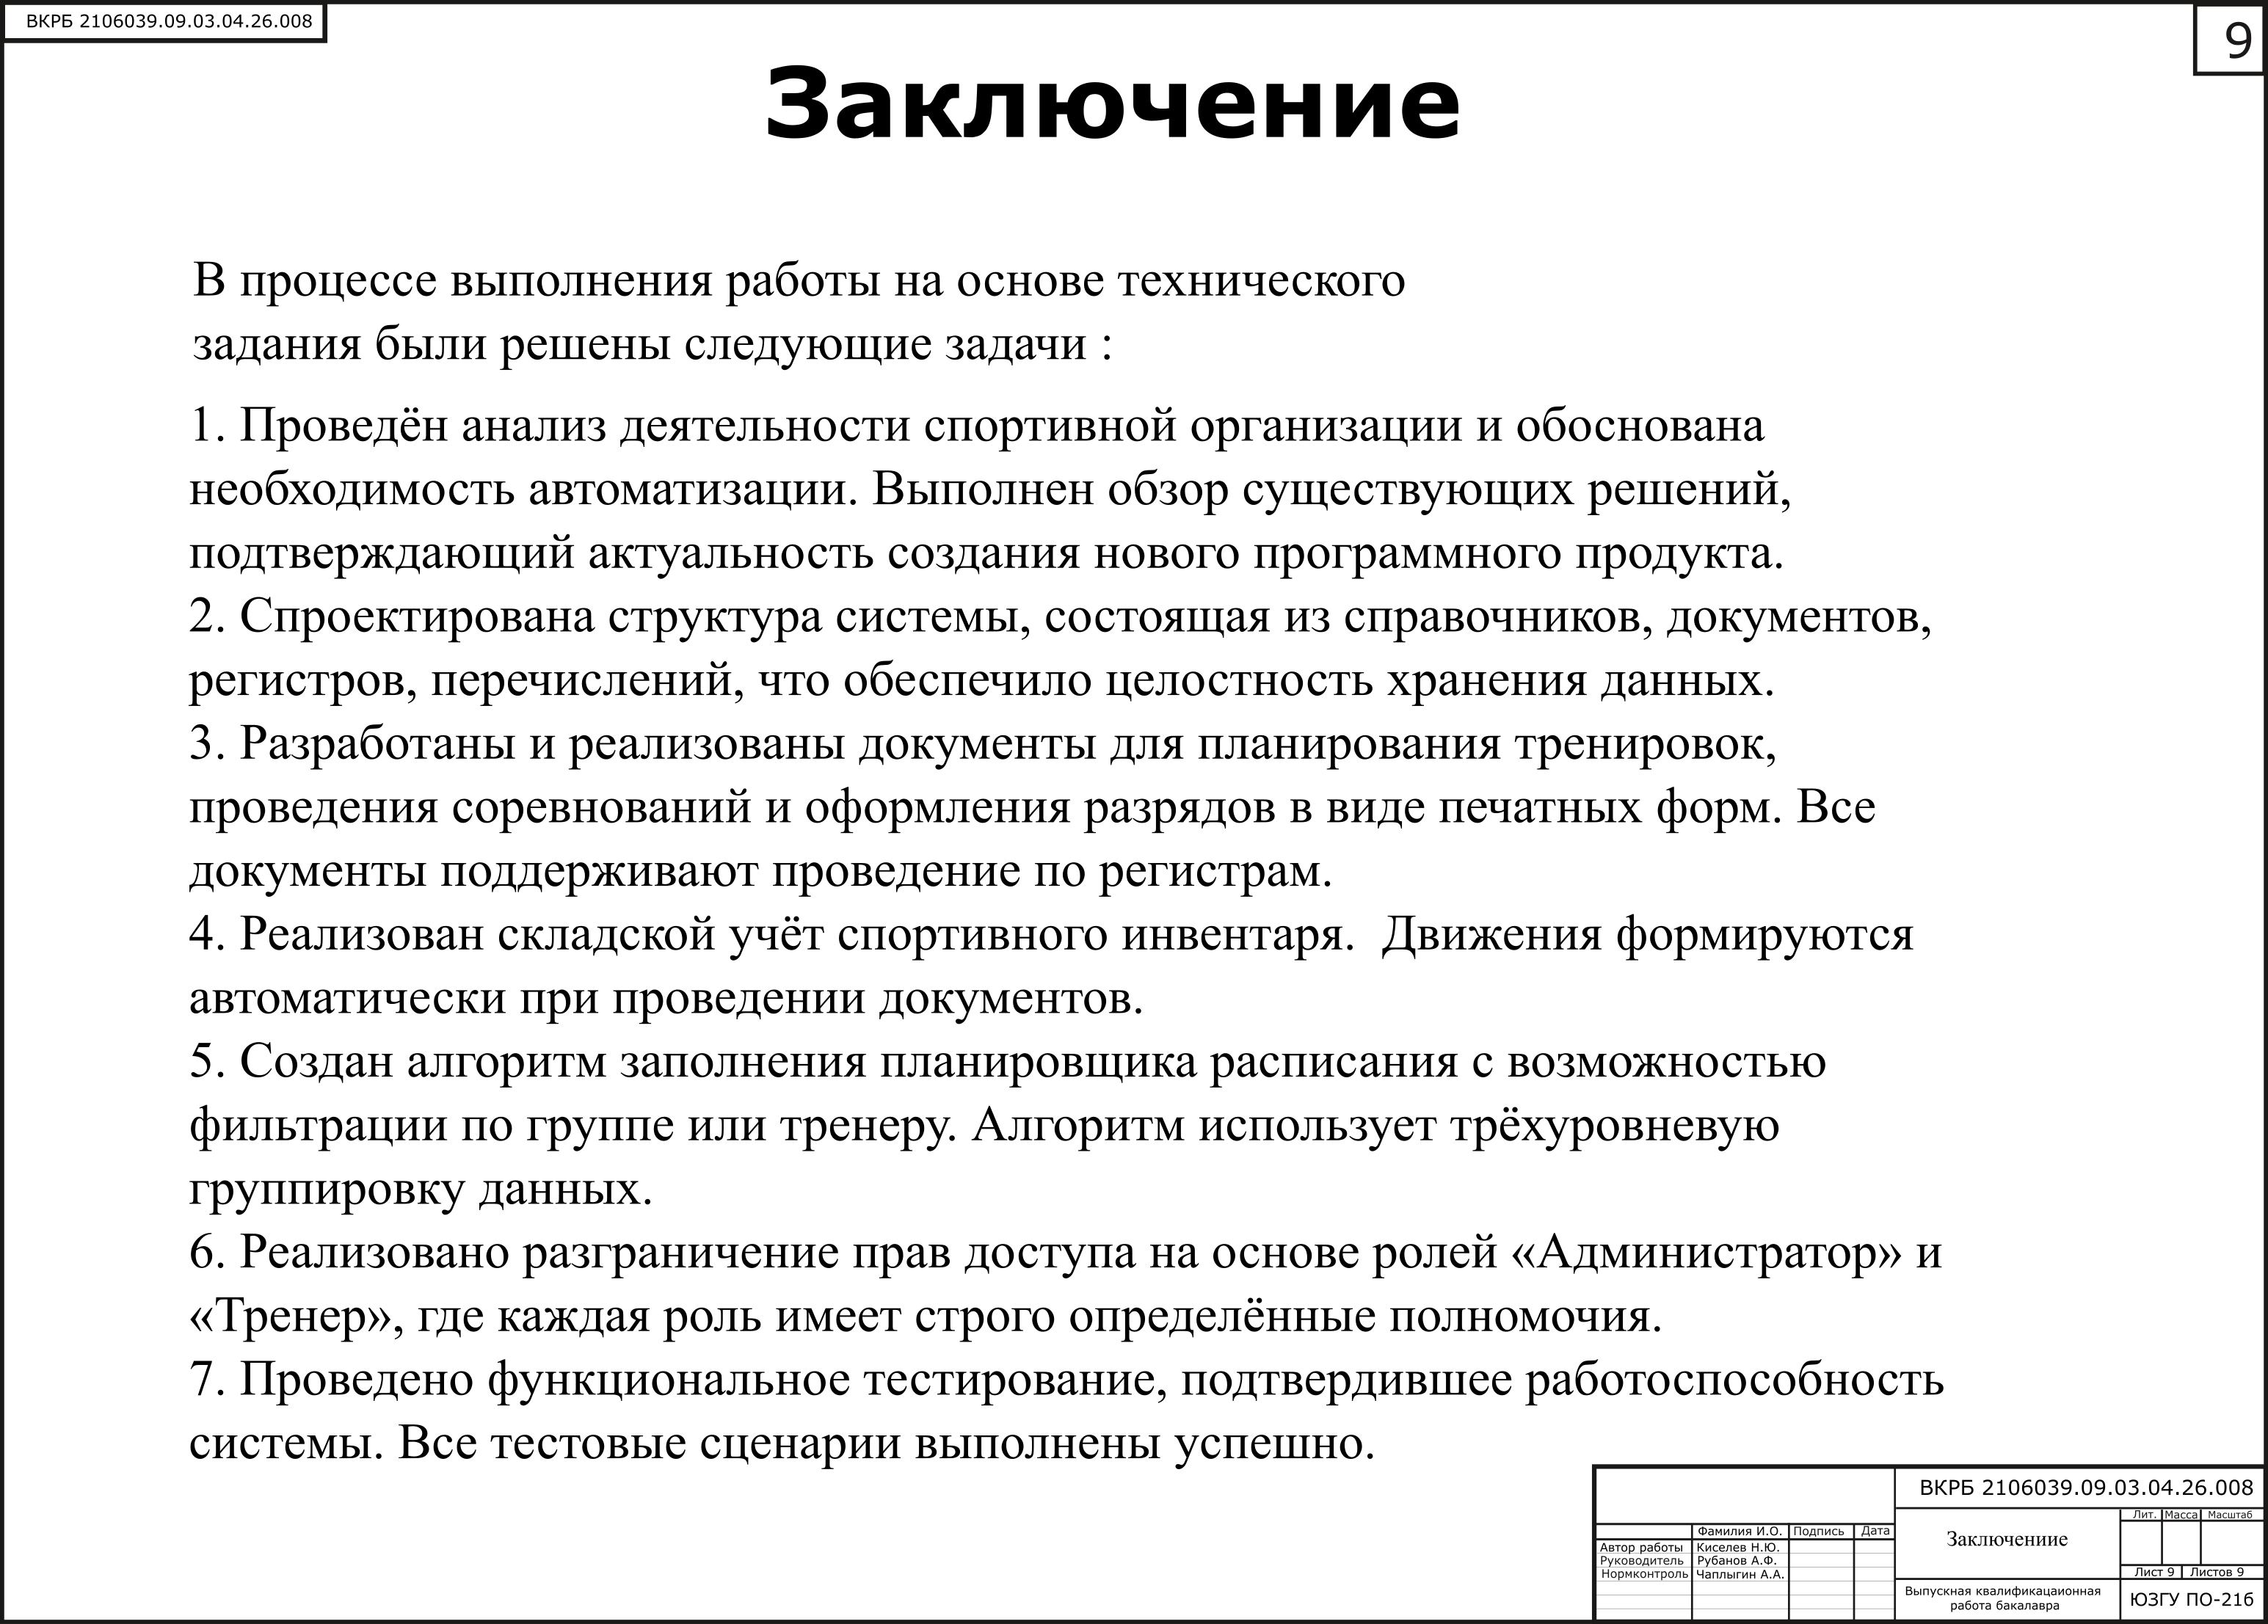
\includegraphics[width=0.85\linewidth]{images/Diplom9.png}
		\заголовок{Заключение}
		\label{pl9:image}      
	\end{плакат}
	
\end{landscape}
}\fi
	\ifПрактика{}\else{\appendix{Фрагменты исходного кода программы}

\subsection*{Модуль формы документа «Соревнования»}
\lstinputlisting[
language=Python,
frame=none,
basicstyle=\ttfamily\small\linespread{1}\selectfont]
{sorev_document.txt}

\subsection*{Модуль формы документа «Результаты соревнования»}
\lstinputlisting[
language=Python,
frame=none,
basicstyle=\ttfamily\small\linespread{1}\selectfont]
{rez_sorev.txt}

\subsection*{Модуль формы документа «Заявка на присвоение разрядов»}
\lstinputlisting[
language=Python,
frame=none,
basicstyle=\ttfamily\small\linespread{1}\selectfont]
{zayavka_razr.txt}

\subsection*{Модуль формы документа «Приказ о присвоении разрядов»}
\lstinputlisting[
language=Python,
frame=none,
basicstyle=\ttfamily\small\linespread{1}\selectfont]
{prikaz_razr.txt}

\subsection*{Модуль формы отчета «Расписание занятий общее»}
\lstinputlisting[
language=Python,
frame=none,
basicstyle=\ttfamily\small\linespread{1}\selectfont]
{raspisanie.txt}

\subsection*{Модуль формы отчета «Расписание занятий группы»}
\lstinputlisting[
language=Python,
frame=none,
basicstyle=\ttfamily\small\linespread{1}\selectfont]
{raspisanie_grupp.txt}

\ifВКР{
\newpage
\addcontentsline{toc}{section}{На отдельных листах (CD-RW в прикрепленном конверте)}
\noindent
\begin{tabular}{p{5.8cm}C{4.8cm}C{4.8cm}}
   Автор ВКР & \lhrulefill{\fill} & \fillcenter\Автор \\
            \setarstrut{\footnotesize}
           & \footnotesize{(подпись, дата)} & \\
            \restorearstrut
   Руководитель ВКР & \lhrulefill{\fill} & \fillcenter\Руководитель \\
            \setarstrut{\footnotesize}
           & \footnotesize{(подпись, дата)} & \\
            \restorearstrut
   Нормоконтроль & \lhrulefill{\fill} & \fillcenter\Нормоконтроль \\
            \setarstrut{\footnotesize}
           & \footnotesize{(подпись, дата)} & \\
            \restorearstrut
\end{tabular}
\vskip 2cm
\begin{center}
\textbf{Место для диска}
\end{center}
}\fi
}\fi
\end{document}